\documentclass[spanish,12pt,letterpaper,titlepage]{report}

\usepackage[spanish]{babel}
\usepackage[T1]{fontenc}
\usepackage[utf8x]{inputenc}
\usepackage{ucs}
\usepackage[scaled]{helvet}
\usepackage[top=1in,bottom=1in,right=1in,left=3cm]{geometry} 
\usepackage{graphicx}
\usepackage{setspace}
\usepackage{rotating}
\usepackage{chngcntr}
\usepackage{multirow}
\usepackage[format=hang,width=.8\textwidth]{caption}
\usepackage[square]{natbib}
\usepackage{wallpaper}

\renewcommand*\familydefault{\sfdefault}
\doublespacing

\counterwithout*{footnote}{chapter}

\author{Gustavo Serrano Diez}
\title{Escuela Salesiana al Alcance de los más Necesitados en Irapuato}

\begin{document}

%\maketitle
\ThisCenterWallPaper{0.8}{images/PORTADA-TESIS-CON-DATOS}
~
\thispagestyle{empty}

\newpage
\ThisCenterWallPaper{0.8}{images/formato-impresion}
\thispagestyle{empty}
~

\newpage
\thispagestyle{empty}
\vspace*{\fill}
\begin{flushright}
	\emph{\textrm{A.M.D.G.}}\\
	\emph{\textrm{(Ad Maiorem Dei Gloriam)}} \\

	\emph{\textrm{Y a todos los que luchan por hacer realidad este sueño}}
\end{flushright}
\vspace*{\fill}


\newpage

\setcounter{page}{1}
\tableofcontents

\chapter{Introducción}
\label{ch:Introduccion}

\section{Conceptualización}

La escuela (salesiana) al alcance de los más necesitados en Irapuato es un bachillerato tecnológico que se pretende crear en dicha ciudad con el doble objetivo de brindar una capacitación técnico-académica de calidad a nivel medio superior y de ofrecer una educación integral en valores según el sistema educativo de Don Bosco a los jóvenes más necesitados.

\subsection{Origen de la Idea}
\label{sub:intro:OrigenIdea}

La idea original nace en el seno de la Comunidad Salesiana <<María Reina de Irapuato>> la cual ante la problemática social enfrentada por las familias en esta ciudad, caracterizada por la ruptura familiar, las adicciones y el analfabetismo, propone la realización de este proyecto, al validar que, ante la interrogante <<¿Qué estamos haciendo por los pobres?>>, no se tiene una respuesta plenamente satisfactoria puesto que las estadísticas locales, la entidad presenta elevados índices en las variables antes mencionadas.\citep{Morales09}

Ante esta situación, el Pbro. Edmundo Morales Romero, S.D.B, sacerdote salesiano miembro de dicha comunidad, destaca la existencia de numerosas razones por las cuales es urgente emprender una labor educativa a fondo y de largo alcance que impacte en el desarrollo local dentro de su ámbito de influencia en primera instancia y en un futuro próximo sea susceptible de reproducción en las demás entidades del país.

Este modelo pretende cubrir desde un sector cuyo nivel económico le permita pagar una colegiatura hasta aquel para el que es del todo imposible hacerlo por si mismo.

Al bachillerato podrán ingresar todos aquellos que hayan acreditado la secundaria. Las clases las tomarán todos juntos evitando todo tipo de discriminación y eliminando una barrera de la historia reciente en nuestro país: la diferencia entre los que van a escuela de paga y a escuela pública.

El perfil de egreso es el de bachillerato de alta calidad con una carrera técnica adecuada a las características de la región.

\subsection{Notas Distintivas}
\label{sub:intro:NotasDistintivas}

La escuela tiene como rasgos distintivos aquellas características del modelo educativo de Don Bosco, y que pueden resumirse en cinco:

\begin{description}
	\item[Sistema preventivo] En contraposición al sistema represivo, se trata de ganar a los estudiantes con amabilidad para orientarlos al bien. A los 9 años, Don Bosco tuvo un sueño en el que Jesús le decía: \emph{no con golpes, sino con la mansedumbre y la caridad deberás ganarte a estos tus amigos}\footnote{San Juan Bosco, Memorias del Oratorio en \citep{Canals95}}.

	\item[Acompañamiento] Los jóvenes nunca están solos, incluso en los ratos de descanso y esparcimiento siempre hay alguien que los acompaña y convive con ellos.
	
	\item[Formación en valores] El sistema preventivo, en palabras de Don Bosco, sólo funciona si se basa en el Evangelio, en una sólida vida interior apoyada en los sacramentos. De aquí se desprende todo lo demás\footnote{San Juan Bosco, en \emph{El Sistema Preventivo en la Educación de la Juventud} (1877) nota 1, \citep{Canals95}. El texto de la nota puede verse íntegro en el Apéndice \ref{ap:preventivo}, página \pageref{ap:preventivo}}.

	\item[Quitar barreras de discriminación] En un mismo salón de clase convivirán jóvenes de todos los estratos sociales, a los cuales se les brindará el mismo trato promoviendo la amistad entre ellos.

	\item[Formación para el trabajo] Mediante las carreras técnicas y los talleres se procurará que los jóvenes tengan la posibilidad de conseguir un empleo ya sea de tiempo parcial para seguir estudiando o si las circunstancias se imponen, de tiempo completo.
\end{description}

\subsection{Contextualización del Proyecto}

El Pbro. Edmundo Morales, S.D.B. solicitó a Gustavo Serrano la asesoría necesaria para llevar a cabo el proyecto. En las diversas conversaciones que tuvieron se establecieron los supuestos sobre los que se trabajaría en el proyecto.\footnote{Ver \ref{sub:Supuestos} más adelante.}

El propósito principal fue el determinar si era posible realizar este proyecto y bajo qué condiciones.

Se añadieron otras necesidades tales como averiguar la situación límite en la que la escuela se sostuviera únicamente con colegiaturas y ofreciera el máximo de becas; de esta forma cualquier donativo o financiamiento externo repercutiría en ampliar la cobertura de becas sin comprometer el funcionamiento de la escuela.

Esta necesidad determinó la línea de realizar los cálculos financieros excluyendo fuentes alternas de financiamiento tales como patrocinios y donativos (a excepción de los de la inversión inicial).

Surgió la discusión acerca de la cobertura mínima de becas aceptable, en un primer momento se planteó que sería <<deseable>> una cobertura del 80\% y como mínimo del 50\%. Al comprobar que esto no era realista se ajustaron los montos tal como se describe en la subsección \ref{sub:Intro:CriteriosExito} <<\nameref{sub:Intro:CriteriosExito}>> (página \pageref{sub:Intro:CriteriosExito}).

Se consideró utilizar el modelo de negocio de un colegio particular promedio con la finalidad de conocer las capacidades y limitaciones de este modelo y tomar los resultados como referencia para ensayar otros modelos en caso de ser necesario.

Debido a las experiencias exitosas en Saltillo y San Luis Potosí,\footnote{Entrevista con el Pbro. Edmundo Morales Romero, S.D.B., 11 de septiembre de 2010} así como la buena reputación de la comunidad salesiana en Irapuato, se consideró como un supuesto válido el contar con el apoyo de patrocinios para la inversión inicial.

En síntesis, el actual trabajo le sirve a la comunidad como instrumento de toma de decisiones y como referencia al momento de establecer la escuela pudiendo realizar ajustes y mejoras.

\section{Objetivos}

\subsection{Objetivo General}
\label{sub:ObjetivoGeneral}

El presente trabajo tiene el siguiente objetivo general:

\begin{quotation}
%	Verificar la viabilidad financiera de la Escuela Salesiana mediante el análisis del punto de equilibrio, indicadores financieros y evaluación financiera para así decidir si se realiza el proyecto como está conceptualizado o se buscan alternativas.
	Verificar la viabilidad financiera de la Escuela Salesiana mediante el análisis de su corrida financiera para así decidir la puesta en marcha del proyecto
	%si se realiza el proyecto como está conceptualizado o se buscan alternativas.
\end{quotation}

%El objetivo general del presente trabajo es verificar la viabilidad financiera de la Escuela Salesiana.

%La viabilidad financiera se entiende en el sentido de que el bachillerato puede ser un negocio redituable.

\subsection{Objetivos Específicos}

El trabajo precisa los siguientes objetivos específicos para garantizar el cumplimiento del objetivo general:

\begin{itemize}
	\item Determinar el monto total de la inversión inicial, mediante el análisis de las necesidades de liquidez e infraestructura, para así establecer la situación patrimonial inicial de la Escuela.
	\item Determinar las fuentes para el financiamiento inicial mediante la diferenciación entre el financiamiento patrocinado y la adquisición de deuda para precisar las obligaciones de largo plazo (pasivos) a cubrir.
	\item Verificar la viabilidad financiera cuidando que siempre se rebase el punto de equilibrio, igualmente, garantizar que las razones financieras indiquen un resultado favorable para así asegurar que la Escuela puede \emph{valerse por sí misma}.
	\item Determinar la cobertura máxima de becas expresada en porcentaje sobre el total de los ingresos mediante el ajuste entre los egresos y los ingresos para así medir a cuántos estudiantes puede beneficiar la escuela si considera como fuentes de ingreso únicamente las de la inversión inicial y las colegiaturas.
	\item Identificar el punto de equilibrio considerando exclusivamente la inversión inicial y las aportaciones de los estudiantes (colegiaturas) para así evaluar la capacidad de la escuela para ofrecer becas.
	\item Verificar si el proyecto, así concebido, es además, rentable desde el punto de vista lucrativo, a través del análisis de las variables de evaluación financiera,\footnote{\label{note:VariablesEvaluacionFinanciera}Período de Recuperación Simple y Descontado, Retorno sobre la Inversión, Valor Presente Neto, Tasa Interna de Rendimiento e Índice de Rentabilidad} lo cual ayudará a la comunidad salesiana de Irapuato a definir su estrategia para la obtención del financiamiento que requiere.\footnote{La estrategia para la obtención del financiamiento externo queda excluida del presente trabajo.}
\end{itemize}

\section{Alcances, Limitaciones y Supuestos del Proyecto}

\subsection{Alcances}
\label{sub:intro:Alcances}

%El presente trabajo abarca únicamente el plan financiero y los aspectos que directa o indirectamente impactan en él.

%¿qué se va a hacer en el trabajo?

Para asegurar el logro de los objetivos antes descritos, el presente trabajo presenta el plan financiero a cinco años de la Escuela Salesiana que se pretende formar.

\subsection{Limitaciones}
\label{sub:intro:Limitaciones}

%%%%%%%%%%%%%%%%%%%%%%%%%%%%%%%%%%%%%%%%%
% se refiere a las limitaciones del trabajo de investigacion/plan financiero, no a las limitaciones del modelo de la escuela salesiana
%%%%%%%%%%%%%%%%%%%%%%%%%%%%%%%%%%%%%%%%%

%- ¿que cosas relacionadas con el objetivo general quedan fuera del trabajo?

%	-- justificacion del objetivo?
%	-- alternativas?
%	-- "como esta conceptualizado" ==> fundamentar ??

%- ¿que cosas relacionadas con los objetivos especificos quedan fuera del trabajo?

%	-- justificacion de la infraestructura?
%	++ viabilidad y origen preciso del financiamiento patrocinado
%	-- institucion crediticia exacta para solicitar el prestamo?
%	-- si el proyecto cumple o no con las condiciones para solicitar el prestamo?
%	-- precicion del termino "favorable" en las razones financieras?
%	-- por que unicamente se consideran las colegiaturas como fuente de ingresos?
%	-- justificacion de las variables de evaluacion financiera?
%	++ la estrategia de la comunidad salesiana para conseguir el financiamiento requerido
%	-- justificacion de la TREMA ?

%- ¿qué qué cosas relacionadas con el alcance quedan fuera del trabajo?

%	-- fuentes para definir la estructura del plan financiero?
%	-- definicion de corrida financiera?
%	-- estudio de mercado "a fondo"?
%	-- justificacion de los criterios de exito?
%	-- la estrategia para conseguir el financiamiento externo

El actual trabajo presenta como limitantes, las que se enumeran a continuación:

\begin{itemize}
	\item Se excluye del presente trabajo la investigación que determine si es viable y bajo qué condiciones las empresas y otros actores sociales patrocinarían el proyecto.
	\item Igualmente queda excluida la estrategia que utilizará la comunidad salesiana para conseguir dichos patrocinios.
	\item No se contemplan fuentes de ingresos adicionales a las especificadas en la inversión inicial y las aportaciones directas de los estudiantes. Aunque se mencionan algunas, únicamente se persigue un propósito ilustrativo, éstas no se consideran para determinar la viabilidad financiera de la escuela.
	\item No se incluye el estudio de mercado que determine el número máximo de personas que se inscribirían a la escuela considerando diferentes montos de colegiatura. % no se si mencionar esta
	\item En cuanto a la cobertura de becas, no se especifica si al 100\% de los estudiantes se les aplica el porcentaje establecido de la beca, o si dicho porcentaje representa la porción del alumnado a los que no se les cobrará nada. La forma concreta de distribuir las becas entre la población estudiantil es materia pendiente de discusión y escapa al alcance de este trabajo.
\end{itemize}

%%%% esto es viejo, ver si se mueve a la prefactibilidad o a otra area %%%%

%El modelo de financiamiento es múltiple: aportaciones directas (colegiaturas), fondos privados, apoyos públicos, servicios a empresas, entre otros.

%Se cobrará una aportación monetaria en función de las capacidades de cada alumno. El objetivo es financiar a los jóvenes de escasos recursos mediante las aportaciones de los estudiantes con posibilidades económicas. Se buscarán fondos privados para becas e infraestructura en diversas modalidades: apadrinar alumnos con buenas calificaciones, apoyos para proyectos específicos: laboratorios, talleres, etc.; apoyos en especie.

%Se intentará obtener apoyos públicos en función de la labor social que se realiza a través de programas como Oportunidades, Practica-Trabaja, Lazos, Bécalos, Prepa Sí, etc.

%Entre otras actividades para obtener ingresos se contemplan: prácticas profesionales patrocinadas por empresas (venta de servicios de acuerdo a carrera técnica y necesidades de las empresas locales); programas de reciclaje; rifas, noches coloniales y eventos de sano entretenimiento, etc.

%Como actividades formativas y simultáneamente ahorradoras se consideran las siguientes: aportaciones en especie de los miembros de la comunidad, jornadas de limpieza, pintura y reparación; servicio en la cooperativa (tienda de la escuela), etc.

\subsection{Supuestos}
\label{sub:Supuestos}

%supuestos: Objeto y materia que no se expresa en la proposición, pero es aquello de que depende, o en que consiste o se funda, la verdad de ella. (recordar en el marco teórico-metodológico)
%- cuáles supuestos tiene el proyecto que lo determinan y que provocaron problemas en la exposición pasada
%- cuáles supuestos tiene el proyecto que lo determinan y aunque no causaron problemas, sí podrían provocarlos en la próxima exposición
%- por qué se dieron estos supuestos

Todo proyecto se apoya en supuestos con la finalidad de cubrir aquellas lagunas que son consecuencia natural de la incertidumbre al momento de realizar la planeación; éstos deberán se confirmados o rechazados durante la puesta en marcha del plan y en dado caso de verificarse falsos, reelaborar el proyecto.

Los supuestos más relevantes en los que se basa este proyecto son los siguientes:

\begin{itemize}
%	\item Se considera que la aprobación por parte de la inspectoría es un hecho aunque podría demorarse, en caso de hacerlo hay que realizar ajustes en el plan, dichos ajustes no se contemplan en el presente trabajo.
	\item Se da por sentado que se contará con los patrocinios y el préstamo necesarios para arrancar el proyecto. La confirmación de este supuesto deberá realizarse a través de sondeos entre posibles patrocinadores y entidades crediticias una vez obtenida la aprobación por parte de los superiores de la congregación salesiana (la inspectoría). Los mencionados sondeos no se incluyen en el presente trabajo.
	\item El modelo de negocio a evaluar es el que generalmente tienen los colegios particulares, con la salvedad de que la inversión inicial incluye un patrocinio y que las utilidades se reinvierten en la misma escuela. Se eligió este modelo con el fin de conocer la capacidad de la escuela de sostenerse y ofrecer becas por sí misma. La exploración de otros modelos no se incluye en este trabajo.
\end{itemize}

\section{Aspectos Metodológicos}
\label{sec:intro:AspectosMetodologicos}

Los aspectos metodológicos que orientan el trabajo se dividen en dos grupos: criterios generales en la elaboración del proyecto y el proceso de elaboración del proyecto.

Los criterios generales buscan delimitar el proyecto en un horizonte de tiempo y precisar el origen y características de la información a obtener.

El proceso para la elaboración del trabajo busca responder a las siguientes preguntas: % siguientes cinco preguntas ?

\begin{enumerate}
	\item ¿Qué se va a hacer en el trabajo?
	\item ¿Cómo se va a realizar?
	\item ¿Qué se espera obtener?
	\item ¿Cuáles son los criterios de éxito?
	\item ¿Cómo se van a interpretar los resultados?
\end{enumerate}

\subsection{Criterios Generales en la Elaboración del Proyecto}

Los criterios generales en la elaboración del proyecto son los siguientes:

\begin{itemize}
	\item El horizonte de evaluación es a cinco años a partir del inicio del proyecto. % copy limitaciones?
	\item Para analizar el mercado y las características de la localidad se recurrirá a documentos ya elaborados e información previamente recopilada, i.e. no se realizarán sondeos ni investigaciones de campo directas. % considerar incluir en la lista de las recomendaciones (a.k.a. conclusiones) la elaboracion de estudios y sondeos en campo.
	\item Todos los datos y cálculos se basan en la información recopilada hasta el año 2010. % % copy limitaciones?
	\item Para la determinación de los costos de los materiales e infraestructura se realizarán cotizaciones con base en la información que ofrecen los diferentes proveedores a través de sus sitios en Internet, buscando obtener el costo promedio.
	\item Para el cálculo del costo de los servicios (agua, luz, etc.), los sueldos y otros gastos, se tomará como referencia los de otros colegios particulares.
	\item El porcentaje de becas a otorgar está en función de la matrícula obtenida, de forma que, a mayor matrícula, mayor cobertura de becas. Dicho porcentaje se incluye en los cálculos mediante su aplicación al monto de la colegiatura \emph{como si se aplicara a la totalidad del alumnado}.\footnote{Revisar \ref{sub:intro:Limitaciones} a partir de la página \pageref{sub:intro:Limitaciones}.}
\end{itemize}

\subsection{¿Qué se va a hacer en el trabajo?}

Como se señaló en los alcances,\footnote{Página \pageref{sub:intro:Alcances}} el presente trabajo consiste en la elaboración del plan financiero a cinco años de la Escuela Salesiana que se pretende formar.

\subsection{¿Cómo se va a realizar?}

Dicho plan contempla la elaboración de una corrida financiera, así como el análisis del punto de equilibrio, las razones financieras y una evaluación financiera del proyecto.

La corrida financiera se basa en la preparación de presupuestos de ingresos y egresos, los cuales, a su vez, se apoyan respectivamente en un análisis preliminar del mercado y en la especificación de las operaciones y necesidades de inversión a realizar. 

El análisis del punto de equilibrio, así como el de las razones financieras y la evaluación financiera provienen de la corrida financiera, principalmente de los estados financieros proforma: estado de resultados, balance general y flujo neto de efectivo.

Siempre que el resultado de la corrida financiera sea favorable, se procurará incrementar el porcentaje de becas para así otorgar un mayor beneficio social. Siendo este proceso iterativo hasta llegar a un porcentaje óptimo.

\subsection{¿Qué se espera obtener?}

Al final se espera obtener la información que permita determinar si el proyecto es viable de acuerdo con los objetivos general y específicos mencionados; más específicamente:

\begin{itemize}
	\item Las utilidades del estado de resultados.
	\item El punto de equilibrio.
	\item Las razones financieras.
	\item El saldo del flujo neto de efectivo.
	\item El valor de las variables de la evaluación financiera.\footnote{Ver nota \ref{note:VariablesEvaluacionFinanciera}, página \pageref{note:VariablesEvaluacionFinanciera}}
\end{itemize}

\subsection{¿Cuáles son los criterios de éxito?}
\label{sub:Intro:CriteriosExito}

Las variables a considerar para determinar el éxito del proyecto, son las razones financieras positivas, las utilidades en el estado de resultados y el saldo positivo en el flujo neto de efectivo.

El porcentaje de las becas correspondiente al nivel de ocupación de la escuela se ajusta a los siguientes criterios:

\begin{itemize}
	\item Si el nivel de ocupación de la escuela es mayor a las $\sfrac{2}{3}$ partes, el porcentaje mínimo aceptable es de 40\%.
	\item Si el nivel de ocupación de la escuela es mayor a $\sfrac{1}{3}$ y menor o igual a $\sfrac{2}{3}$, el porcentaje mínimo aceptable es de 30\%.
	\item Si el nivel de ocupación de la escuela es menor o igual a $\sfrac{1}{3}$, el porcentaje mínimo aceptable es de 20\%.
\end{itemize}

El valor de las variables de la evaluación financiera no se considera como criterio de éxito o fracaso del proyecto.

%De los cinco años que se están analizando, al menos los tres últimos deben arrojar utilidades (estado de resultados, rebasar el punto de equilibrio), y tener valores aceptables en las razones financieras; en cuanto al flujo neto de efectivo, al menos el último año debe ser positivo, lo cual significa que la escuela recupero completamente su inversión. % cuando se haga chido el proyecto (fase 5) considerar esto

\subsection{¿Cómo se van a interpretar los resultados?}

Los resultados de la corrida financiera se interpretarán de la siguiente forma:

Considerando los pocentajes de beca mínimos aceptables, si el proyecto rebasa el punto de equilibrio (i.e. el estado de resultados tiene saldo positivo), las razones financieras son positivas y al final el flujo neto de efectivo es positivo; entonces el proyecto es viable. Si falla alguno de estos tres criterios, entonces se debe replantear el modelo.

En cuanto a la evaluación financiera,\footnote{Ver nota \ref{note:VariablesEvaluacionFinanciera}, página \pageref{note:VariablesEvaluacionFinanciera}} ésta cumple otro propósito, mientras mejores sean los resultados arrojados por estas variables, más fácil será obtener el financiamiento y apoyo requerido; si los resultados no son favorables, deberá realizarse un mayor esfuerzo en la elaboración y ejecución de la estrategia de la búsqueda de apoyo y financiamiento externos.

\section{Prefactibilidad}

\subsection{Aspectos Previos - Situación Actual}
\label{sub:Intro:AspectosPrevios}

El estado de Guanajuato enfrenta diversos problemas sociales derivados de una oferta educativa insuficiente:
%(Cf. \citep{Morales09}):

\begin{description}
	\item[Educación] Guanajuato es una de las entidades con mayor índice de analfabetismo a nivel nacional.\footnote{Según el Conteo de Población y Vivienda 2005 \citep{Inegi2005}, Guanajuato ocupa el quinto \emph{último} lugar en escolaridad con 7.1 años en promedio contra 8.1 nacional.} Concentrándose la mayor cantidad de analfabetas \emph{en las zonas urbanas}.\footnote{\citep{Morales09}}
	\item[Desempleo] El desempleo asciende al 6\% de la población económicamente activa.\footnote{\citep{Inegi2010Enoe}}
	\item[Niños de la calle] Guanajuato es de los principales estados receptores de niños de la calle.\footnote{\citep{Morales09}}
	\item[Ruptura familiar]
	Guanajuato pasó del lugar 22º al 19º nacional en divorcios entre los años 2005 y 2009\footnote{Comparar \citep{Inegi2005pGto} con \citep{Inegi2009pGto}} con el consecuente semi abandono de los niños.\footnote{\citep{Morales09}}
	%Guanajuato está en el 4º lugar de divorcios, ha aumentado un 400\% en estos últimos años, con el consiguiente semi abandono de los niños.
	\item[Delincuencia] Al igual que el resto del país, la entidad padece un incremento en los índices delictivos y de violencia.\footnote{\citep{CIDE2010}}
\end{description}

\subsection{En Caso de no Llevarse a Cabo}

En caso de no llevarse a cabo el proyecto, estos índices aumentarían con grave daño a la sociedad local.

Por otra parte, el gran desarrollo industrial del Estado se vería afectado y la comunidad no podría aprovechar este beneficio, al no contar con la preparación técnica necesaria, las empresas contratarían personal foráneo para cubrir sus necesidades de talento humano.

\subsection{Ubicación}

Se cuenta con un inmueble ubicado en la zona centro de Irapuato, abarca toda la manzana delimitada por las calles: Díaz Ordaz, Francisco Sarabia, Río Grijalba y Lázaro Cárdenas, se puede observar una foto satelital en la figura \ref{fig:ubicacion}.

\begin{figure}
	\centering
	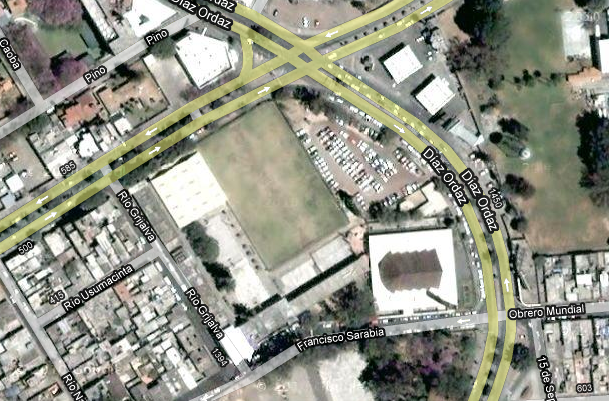
\includegraphics[scale=0.5]{images/localizacion}
	\caption[Fotografía satelital y ubicación del inmueble.]{Fotografía satelital y ubicación del inmueble.\newline Fuente: \citep{GoogleMaps2010}}
	\label{fig:ubicacion}
\end{figure}

\subsection{Evaluación Financiera Previa}

\subsubsection{Infraestructura Actual}

Se cuenta con un inmueble adaptado como escuela, al cual, actualmente no se le da este uso; aunque requerirá modificaciones menores ya tiene la capacidad de atender a más de 1,000 alumnos en 40 aulas.

La superficie del inmueble es de 14,452 $m^2$ con un valor aproximado de \$ 3.4 millones de pesos; los edificios están valuados en \$ 2.4 millones de pesos aproximadamente.

%\footnote{Valor estimado con base en el precio por metro cuadrado promedio en Irapuato \citep{AM2010}}.

\subsubsection{Beneficio Social}
\label{sub:sub:Beneficio:Social}

Considerando la capacidad actual del inmueble el beneficio social que se espera obtener es el equivalente a 400 jóvenes atendidos de forma completamente gratuita. Sin embargo, la intención es distribuir las becas utilizando porcentajes, por lo que el número total de estudiantes becados se espera sea mayor.\footnote{Ver la subsección \ref{sub:intro:Limitaciones} a partir de la página \pageref{sub:intro:Limitaciones}.} Por comparación, un bachillerato salesiano en Jalisco orientado como \emph{escuela privada} otorga un 20\% en becas.

Por otra parte, la educación en valores basada en el sistema preventivo de Don Bosco beneficiará todos los estudiantes y a sus familias.

\subsubsection{Capacidad actual}

Se pretende dividir a los alumnos en grupos de 30 estudiantes como máximo. De acuerdo con el sistema salesiano, esto da como resultado un total de 37 personas atendiendo directamente a los estudiantes.

%La colegiatura estándar en la región es de \$3,000.00 mensuales, lo cual, aplicado a 600 estudiantes durante un año da como resultado un monto de \$21,600,000.00. A esta cantidad habrá que añadir lo que se obtenga mediante donativos y patrocinios.

\subsubsection{Patrocinios}
\label{sub:Patrocinios}

Las experiencias similares en Saltillo y San Luis Potosí\footnote{Entrevista con el Pbro. Edmundo Morales Romero, S.D.B., 11 de septiembre de 2010} muestran que esta clase de proyectos son bien recibidos por los industriales locales; en efecto, en ambas entidades, los grupos industriales realizaron aportaciones en efectivo y en especie a tal grado que incluso donaron los terrenos a cambio de adaptar los planes de estudio a sus necesidades.

Irapuato se ubica en el centro del eje industrial de Guanajuato, el cual incorpora a las ciudades de León, Silao, Irapuato y Salamanca. En toda esta zona existen diversos parques industriales e industrias de todo tipo. Próximamente se abrirá una planta de fabricación de componentes espaciales, la cual estará necesitada de mano de obra calificada. Todas estas industrias son candidatos a ser patrocinadores del proyecto por así convenir a sus intereses.


\chapter{Administración de Negocios}
\label{ch:AdministracionNegocios}

\section{Necesidades del Mercado}

Las necesidades del mercado se pueden revisar desde tres aspectos: rezago educativo, problemas sociales y necesidades de otros actores involucrados (empresas y gobierno). Posteriormente se revisan algunas tendencias y al final se incluye un apartado sobre nuestra propuesta de valor considerando esta problemática.

\subsection{Rezago Educativo}

Como se señaló en la subsección \ref{sub:Intro:AspectosPrevios} (página \pageref{sub:Intro:AspectosPrevios}), Guanajuato es una de las entidades con mayor rezago educativo del país. Paradójicamente existe un gran desarrollo industrial que abarca desde León hasta Salamanca.\footnote{Por ejemplo, en Silao se encuentra una de las plantas de General Motors}

Según el conteo de población y vivienda de 2005 \citep{Inegi2005}, la población total entre 15 y 19 años en el municipio de Irapuato, fue de 47,177 jóvenes, de los cuales 22,117 asistían a la escuela, lo cual representa un 46\%. Más aun, la misma fuente informa que de 16,086 jóvenes comprendidos en esas edades con secundaria terminada, únicamente 14,623 asisten al bachillerato (ver el cuadro \ref{tbl:INEGI:PoblacionEstudiaIrapuato}); hecho confirmado por la Secretaría de Educación de Guanajuato (SEG), según la cual, la matrícula de bachillerato en 2005 fue de 15,687 estudiantes y en 2009 de 17,734 (\citep{Seg2010}).

\begin{table}
	\centering
    \caption{Datos Generales de Poblaci\'on}
    \label{tbl:INEGI:PoblacionEstudiaIrapuato}
    \begin{tabular}{p{4in}|r|r}
        \multicolumn{1}{c|}{VARIABLE}
        	& \multicolumn{1}{c|}{2000$^{/a}$}
        	& \multicolumn{1}{c}{2005$^{/b}$} \\
        \hline \hline
        Poblaci\'on total & 440,134 & 463,103 \\
        Poblaci\'on de 15 a 19 a\~nos & 45,325 & 47,177 \\
        Poblaci\'on de 15 a 19 a\~nos que asiste a la escuela & 17,607 & 22,117 \\
        Poblaci\'on de 15 a 19 a\~nos con secundaria terminada & 12,688 & 16,086 \\
        Poblaci\'on de 15 a 19 a\~nos con estudios de bachillerato$^{/c}$ & 10,109 & 14,623 \\
        \hline
        \multicolumn{3}{l}{$^{/a}$ \footnotesize Fuente: \citep{Inegi2000}} \\
        \multicolumn{3}{l}{$^{/b}$ \footnotesize Fuente: \citep{Inegi2005}} \\
        \multicolumn{3}{p{5.4in}}{$^{/c}$ \footnotesize No especifica si est\'a cursando o ya curs\'o, por el desglose de cada a\~no dentro del grupo de edad de 15 a 19 a\~nos se intuye que se refiere a ``cursando''}
    \end{tabular}
\end{table}


Entre 2005 y 2009, se promedió anualmente un aproximado de 830 egresados de secundaria que no ingresaron a bachillerato. En el mismo periodo, el índice de aprobación en bachillerato fue de 58\%; el número de egresados de secundaria se incrementó anualmente 2.3\% en promedio; el de nuevos ingresos a bachillerato fue de 1.82\% y el de egresos fue de 1.75\% \citep{Seg2010}\footnote{Ver los cuadros \ref{tbl:SEG:Secundaria} y \ref{tbl:SEG:Bachillerato}}.

¿Por qué tan pocos jóvenes estudian? Una primera explicación es la común para estos casos: \emph{Los jóvenes de escasos recursos abandonan la escuela porque tienen que trabajar para sostener a su familia; encuentran dificultades para emplearse dignamente pues carecen de los conocimientos necesarios. Para muchos, estudiar una carrera universitaria se vuelve un privilegio.}

El Consejo Nacional de Evaluación de la Política de Desarrollo Social (CONEVAL) informa que Irapuato es el quinto municipio con menor índice de pobreza del estado, con un 47\% de población en pobreza patrimonial, 21\% en pobreza de capacidades y 14\% en pobreza alimentaria \citep{Coneval2009} (cuadro \ref{tbl:CONEVAL:MunicipiosPobreza}).

Una segunda explicación proviene de la falta de espacios educativos; en efecto, según la Secretaría de Educación de Guanajuato \citep{Seg2010}, mientras  Irapuato mantiene desde el ciclo esclolar 2004-2005 a la fecha, un índice de absorción escolar promedio de 88\%\footnote{\emph{Absorción}: proporción de alumnos de nuevo ingreso a primer grado de un nuvel educativo, respecto a los alumnos egresados del nivel y ciclo inmediato anterior \citep{Seg2010}.};
municipios como Tierra Blanca o Celaya, mantienen un promedio superior a 110\% en el mismo periodo.

\begin{table}
    \centering
    \caption{Egresados de Secundaria en el Municipio de Irapuato}
    \label{tbl:SEG:Secundaria}
    \begin{tabular}{c|c||l|r}
        AÑO & EGRESADOS & \multicolumn{1}{c|}{INDICADOR}
            & \multicolumn{1}{c}{VALOR} \\
        \hline \hline
        2005 & 7,515 & Acumulado       & 38,560  \\
        2006 & 7,561 & Promedio        &  7,712  \\
        2007 & 7,306 & Incremento      &  177.4  \\
        2008 & 7,991 & Incremento \%   &  2.30\% \\
        2009 & 8,187 & Proyectado 2010 &  8,244  \\
        \hline
        \multicolumn{4}{l}{\footnotesize Fuente: \citep{Seg2010}}
    \end{tabular}
\end{table}


\begin{table}
    \centering
    \caption{Indigadores Generales del Bachillerato en Irapuato}
    \footnotesize
    \label{tbl:SEG:Bachillerato}
    \begin{tabular}{c|r|r|r|r}
        AÑO  & NUEVO INGRESO & EGRESADOS & MATRICULA & APROBACION \\
        \hline \hline
        2005 & 6,716 & 3,856 & 15,687 & 57\% \\
        2006 & 7,112 & 3,882 & 16,242 & 55\% \\
        2007 & 6,353 & 3,797 & 15,457 & 60\% \\
        2008 & 6,669 & 4,228 & 15,682 & 63\% \\
        2009 & 7,564 & 3,969 & 17,374 & 52\% \\
        \hline
        \multicolumn{5}{c}{INDICADORES} \\
        \hline
        \multicolumn{1}{l|}{Acumulado}       & 34,414  & 19,732  & 80,442 &     N/A \\
        \multicolumn{1}{l|}{Promedio}        &  6,883  &  3,946  & 16,088 &    58\% \\
        \multicolumn{1}{l|}{Crecimiento}     &  125.3  &  57.2   &  281.4 & -0.11\% \\
        \multicolumn{1}{l|}{Crecimiento \%}  &  1.82\% &  1.45\% & 1.75\% & -0.19\% \\
        \multicolumn{1}{l|}{Proyectado 2010} &  7,259  &  4,118  & 16,933 &    57\% \\
        \hline
        \multicolumn{5}{l}{\footnotesize Fuente: \citep{Seg2010}}
    \end{tabular}
\end{table}

\begin{table}
    \centering
    \caption[Municipios con Mayor y Menor Grado de Pobreza por Ingresos]{Municipios con Mayor y Menor Grado de Pobreza\newline por Ingresos}
    \label{tbl:CONEVAL:MunicipiosPobreza}
    \footnotesize
    \begin{tabular}{c|l|r||c|c|c}
                       &                &           & POBREZA     & POBREZA DE  & POBREZA DE \\
                       & MUNICIPIO      & POBLACIÓN & ALIMENTARIA & CAPACIDADES & PATRIMONIO \\ 
        \hline \hline
        Estatal        & Guanajuato     & 4,893,812 & 18.9 \%     & 26.6 \%     & 51.6 \%    \\ 
        \hline
        Municipios     & Xichú          &    10,592 & 60.8 \%     & 68.5 \%     & 83.6 \%    \\ 
        con mayor      & Atarjea        &     5,035 & 58.8 \%     & 67.1 \%     & 83.2 \%    \\ 
        porcentaje     & Tierra Blanca  &    16,136 & 50.9 \%     & 59.4 \%     & 77.3 \%    \\ 
        de pobreza     & Victoria       &    19,112 & 47.4 \%     & 55.4 \%     & 73.2 \%    \\ 
                       & Santa Catarina &     4,544 & 41.3 \%     & 47.8 \%     & 64.4 \%    \\ 
        \hline
        Municipios     & Irapuato       &   463,103 & 14.0 \%     & 21.2 \%     & 46.9 \%    \\ 
        con menor      & Uriangato      &    53,077 & 11.6 \%     & 19.9 \%     & 50.4 \%    \\ 
        porcentaje     & Celaya         &   415,869 & 11.5 \%     & 17.9 \%     & 41.3 \%    \\ 
        de pobreza     & Moroleón       &    46,751 &  9.5 \%     & 16.1 \%     & 42.6 \%    \\ 
                       & León           & 1,278,087 &  7.9 \%     & 13.6 \%     & 38.2 \%    \\ 
        \hline
        \multicolumn{6}{l}{\footnotesize Fuente: \citep{Coneval2009}}
    \end{tabular}
\end{table}


Otro indicador importante es la atención a la demanda estatal \footnote{\emph{Atención a la demanda estatal}: Valores cercanos a 100 implican que el sector educativo atiende a la mayoría de la población en edad escolar que demande este servicio \citep{Seg2010}}, Irapuato mantiene del ciclo escolar 2004-2005 al ciclo 2009-2010 un promedio de 81\%, municipios como Uriangato o Tierra Blanca tienen más del 90\%. En el último ciclo escolar, el municipio de Atarjea obtuvo 120\% en este indicador.

Según estas cifras, a nivel bachillerato, el municipio no ha cubierto el total de la demanda educativa, ante este escenario, los jóvenes buscan alternativas en otro sitio o simplemente abandonan la escuela.

Finalmente está la valoración de la educación; muchas personas consideran que con saber leer y escribir y hacer cuentas basta; este fenómeno se da particularmente entre quienes se dedican al comercio y elaboración de productos artesanales. Para estas personas, la educación superior es un saber que no aporta valor económico, muy teórico y alejado de sus necesidades.\footnote{Convendría realizar un estudio de mercado más afondo sobre este tema, dicho estudio rebasa el alcance de este proyecto.}

\begin{table}
	\centering
    \caption{\'Indices de Absorci\'on y de Atenci\'on a la Demanda Estatal}
    \label{tbl:SEG:AbsorcionYDemandaEstatal}
    \footnotesize
    \begin{tabular}{l||r|r|r|r|r|r||r}
        \hline
        \hline
                      & \multicolumn{7}{|c}{ABSORCION}                                                  \\
        \hline
        MUNICIPIO     & 04-05     & 05-06     & 06-07     & 07-08     & 08-09     & 09-10     & PROMEDIO \\
        \hline
        Estado        &  80.40\%  &  83.00\%  &  87.80\%  &  84.90\%  &  86.00\%  &  86.40\%  &  84.75\% \\
        Tierra Blanca & 125.00\%  & 130.90\%  & 133.30\%  & 115.40\%  & 119.10\%  & 120.50\%  & 124.03\% \\
        Celaya        & 106.50\%  & 108.60\%  & 121.30\%  & 113.60\%  & 120.00\%  & 117.60\%  & 114.60\% \\
        Irapuato      &  88.60\%  &  89.40\%  &  94.10\%  &  87.00\%  &  83.50\%  &  85.70\%  &  88.05\% \\
        \hline
        \hline
                      & \multicolumn{7}{|c}{ATENCION A LA DEMANDA ESTATAL}                    \\
        \hline
        MUNICIPIO     & 04-05   & 05-06   & 06-07   & 07-08   & 08-09    & 09-10    & PROMEDIO \\
        \hline
        Estado        & 76.90\% & 77.90\% & 82.20\% & 79.00\% &  81.10\% &  81.00\% & 79.68\%  \\
        Uriangato     & 84.20\% & 90.10\% & 94.30\% & 87.50\% & 147.30\% &  88.20\% & 98.60\%  \\
        Tierra Blanca & 89.00\% & 95.40\% & 90.20\% & 86.40\% &  97.40\% &  88.50\% & 91.15\%  \\
        Atarjea       &  0.00\% &  0.00\% &  0.00\% &  0.00\% &  20.00\% & 119.80\% & 23.30\%  \\
        Irapuato      & 81.20\% & 81.30\% & 83.90\% & 78.30\% &  81.60\% &  80.50\% & 81.13\%  \\
        \hline
        \multicolumn{8}{l}{Fuente: \citep{Seg2010}}
    \end{tabular}
\end{table}


\subsection{Problemas Sociales}

Se mencionan dos problemas sociales derivados de una inadecuada educación: la ruptura familiar y la desigualdad de oportunidades por relaciones humanas.

La ruptura familiar provoca desorientación y violencia en la juventud; existen muchos j\'ovenes que caen en las drogas con todos los problemas que ello implica\footnote{Entrevista del autor con el Pbro. Edmundo Morales, S.D.B., 16 de octubre de 2010}; la causa es la falta de valores: la falta de orientación y valores en la juventud los incapacita para afrontar la vida con integridad, los vuelve vulnerables a diversas formas de manipulación y violencia. Es significativo el elevado índice de divorcios en la entidad, síntoma de una falta de capacidad de establecer relaciones estables y compromisos duraderos\footnote{Cf. \citep{Morales09}}.

En un diagnóstico reciente, la comunidad salesiana local identificó la drogadicción como un problema entre muchos jóvenes, así como el aumento de pandillas y violencia en las calles. Consideran que la educación de esos jóvenes es el camino para resolver esos problemas\footnote{Diagnóstico interno de la comunidad, 2010}.

Otro problema muy grave es la desigualdad en cuanto a oportunidades se refiere\footnote{Aquí no se hace referencia a los índices de desigualdad social sino a un aspecto cualitativo del problema: las relaciones humanas}. La división entre los que van a una escuela de paga y los que van a escuela de gobierno, entre la gente <<bien>> y el <<pueblo>>, provoca un serio problema de discriminación alimentado por prejuicios que al final lo que produce es que unos cuantos se beneficien del conocimiento y las relaciones personales para obtener empleo y el resto tenga serias dificultades a pesar de que en muchos casos existe talento y compromiso.

\subsection{Otros Actores Involucrados}

Las empresas necesitan personal capacitado y competente, la educación formal es insuficiente, pues no ha mostrado capacidad de adaptarse al dinamismo del mundo laboral.

Finalmente, los gobiernos de los tres órdenes (federal, estatal y municipal) enfrentan un grave reto ante los elevados índices de analfabetismo que entran en conflicto con el creciente desarrollo industrial, el riesgo es que las empresas contraten <<personal de fuera>> y los habitantes de la región se vuelvan <<meros expectadores del progreso>>.

\subsection{Tendencias identificadas}

Se han identificado las siguientes tendencias:

\begin{itemize}
	\item En cuanto al rezago educativo, tanto los gobiernos como la sociedad han realizado notables esfuerzos por superar el rezago educativo. Aun así, todavía resulta insuficiente.
	\item Por otra parte, las empresas requieren de manera creciente los servicios de personal mejor capacitado, esto para afrontar un ambiente global cada vez más competitivo. \emph{La verdadera preparación para el trabajo comienza en el trabajo mismo}.
	\item La crisis de valores se acentúa en proporción directa con la desintegración familiar, el incremento de la violencia y el desmoronamiento del tejido social. Es cada vez mayor el número de jóvenes y adultos que carecen de un criterio orientador de su vida, lo cual los vuelve incapaces de asumir compromisos duraderos y frágiles en el momento de enfrentar la tentación de elegir el camino más fácil en lugar del camino correcto.
	\item Existe una mayor demanda de espacios educativos la cual ha sido atendida con insuficiencia por parte de los gobiernos y otros actores de la sociedad.
\end{itemize}

\subsection{Propuesta de Valor}

Para los jóvenes de la región un bachillerato de calidad y una carrera técnica; para los de escasos recursos, ofrecemos un precio accesible con posibilidad de becas y financiamiento que les permita encontrar un empleo y continuar con una carrera universitaria.

Una formación en valores que les permitan afrontar con entereza las dificultades de la vida, convirtiéndose en \emph{buenos cristianos y honestos ciudadanos}.\footnote{Lema escogido por Don Bosco para sus escuelas}

Trato igual y convivencia entre los que pagan colegiatura y los que no, una convivencia que supere los prejuicios entre clases sociales y elimine las barreras de discriminación.

Para las empresas contar con talento humano adecuado a sus necesidades adaptando el plan de estudios y ofreciendo carreras técnicas adecuadas a las necesidades laborales más apremiantes.

Para los gobiernos reducir los índices de analfabetismo, rezago educativo y desempleo: y a largo plazo, los índices de violencia y ruptura familiar.

\section{Clientes}
\label{sec:Clientes}

\subsection{Pirámide de Necesidades del Mercado}

En la base se encuentra el grupo más numeroso, constituido por jóvenes entre 15 y 19 años de edad, con secundaria terminada y deseosos de continuar sus estudios.

Inmediatamente después están los padres de familia, preocupados por la educación de sus hijos y que reciban valores.

Un grupo importante es el de las empresas, interesadas en disponer de mano de obra calificada.

En la cúspide se encuentran los gobiernos de los tres órdenes (federal, estatal y municipal), quienes tienen interés en reducir los índices de analfabetismo y rezago educativo.

El proyecto se enfoca principalmente a los dos primeros grupos (jóvenes y padres de familia), de quienes se presentan sus perfiles a continuación.

\subsection{Grupos de clientes}

\subsubsection{Jóvenes}

En Irapuato, los j\'ovenes entre 15 y 19 a\~nos de edad con secundaria terminada conforman un grupo de aproximadamente 16,086 integrantes \citep{Inegi2005}. La mayor\'{i}a sigue estudiando el bachillerato. Entre sus gustos e intereses est\'a el deporte; especialmente el futbol. La afici\'on del Irapuato es fuerte en el municipio\footnote{Entrevista del autor con el Pbro. Edmundo Morales, S.D.B., 16 de octubre de 2010}. Otros intereses de los j\'ovenes son el cine, la m\'usica y las fiestas \citep{Cordero07}.

Entre los intereses de los jóvenes está el estudio, pues muchos cambian de ciudad en busca de espacios educativos\footnote{Entrevista del autor con el Pbro. Edmundo Morales, S.D.B., 16 de octubre de 2010}.

Para efectos de la estrategia a seguir, se utilizarán los parámetros como unidad de segmentación.

La escuela busca cubrir un amplio espectro de jóvenes, los cuales se pueden ubicar en un espectro que va desde los que tienen una posición económica acomodada que les permite pagar una costosa educación, hasta los que abandonan la escuela por falta de medios económicos.

%Algunos grupos de estudiantes, de acuerdo a su criterio de elección escolar, son:
%\begin{itemize}
%	\item
%	Quienes buscan un colegio particular de prestigio
%	\item
%	Quienes buscan un colegio particular a precios más accesibles que el promedio
%	\item
%	Quienes no encontraron cupo en el sistema oficial y no tienen medios económicos para inscribirse a un colegio particular
%	\item
%	Quienes desean prepararse para el trabajo, sea porque desean pagar sus estudios universitarios trabajando o bien porque necesitan encontrar un buen trabajo para sostener a su familia.
%\end{itemize}

\subsubsection{Padres de familia}

Los padres de familia están interesados en procurar un mejor futuro a sus hijos. Forma parte de la mentalidad local que el camino a un mejor progreso es estudiar una carrera universitaria, en ese sentido, las carreras exclusivamente técnicas no son apreciadas\footnote{Entrevista del autor con el Pbro. Edmundo Morales, S.D.B., 16 de octubre de 2010}.

Uno de los problemas que enfrentan los padres de familia es el costo de las colegiaturas. Según la Encuesta de Ingresos y Gastos de los Hogares 2008 Guanajuato\footnote{\citep{INEGI-2009-DGES-003}}, el gasto promedio en educaci\'on por miembro de la familia es de \$ 235.20, siendo el m\'as bajo de \$ 0.00 y el m\'as alto de \$ 7,900.00.

Considerando que el bachillerato oficial cuesta \$ 3,000.00 al semestre (m\'as de \$ 500.00 mensuales) y los colegios particulares oscilan alrededor de los \$ 3,000.00 mensuales; resulta una verdadera preocupaci\'on para los padres de familia el cubrir los gastos de la educaci\'on de sus hijos.

Otro aspecto a considerar es la educacin en valores; Guanajuato tiene una población 96\% católica cuya característica es apreciar los valores de su fe\footnote{Inegi2000}. Es una sociedad, en este aspecto, tradicional\footnote{Entrevista del autor con el Pbro. Edmundo Morales, S.D.B., 16 de octubre de 2010}, uno de los centros religiosos más importantes del país se encuentra a pocos kilómetros de Irapuato\footnote{El santuario de Cristo Rey, ubicado en la cima del Cerro del Cubilete en Silao, Gto.; son emblemáticas las peregrinaciones juveniles que se realizan en enero cada año con repercusión en la prensa nacional y local}, ese centro recibe miles de peregrinos durante todo el año, tanto locales como de otras entidades; siendo también un importante centro turístico.

%En conclusión, se enlistan algunos grupos de padres de familia:
%
%\begin{itemize}
%	\item
%	Aquellos que buscan una educación de calidad para sus hijos
%	\item
%	Aquellos que desean que sus hijos reciban una preparación para el trabajo además del bachillerato
%	\item
%	Aquellos interesados en que sus hijos reciban valores y se formen como buenos cristianos
%	\item
%	Aquellos que no pueden pagar un bachillerato a sus hijos y desean que sigan estudiando
%\end{itemize}

\subsection{Perfilamiento}

Se identifican los siguientes parámetros de perfilamiento, tanto para estudiantes como para padres de familia, los mismos servirán como perfiles de clientes para efectos del presente trabajo:

\begin{description}
	\item [Posición económica] la decisión se basa en la economía
	\item [Interés académico] la decisión se basa en la calidad educativa, prestigio o calidad técnica
	\item [Interés laboral] la decisión se basa en ser un medio para obtener empleo
	\item [Orientación religiosa] se elige una escuela que vaya acorde con sus convicciones religiosas y valores
	\item [Otros intereses] ambiente, valores, cultura, actividades, facilidad, etc
\end{description}

Mediante estos parámetros se pueden identificar varios grupos de estudiantes:

\begin{itemize}
	\item Quienes buscan un colegio particular dentro de las posibilidades de pago (posición económica)
	\item Quienes buscan un colegio oficial porque uno particular está fuera de su alcance (posición económica)
	\item Quienes no alcanzaron cupo en el sistema oficial (posición económica)
	\item Quienes buscan ingresar al sistema oficial por su nivel académico (interés académico)
	\item Quienes buscan una preparación técnica sólida (interés académico)
	\item Quienes buscan un colegio particular de prestigio (interés académico)
	\item Quienes demandan capacitación para el empleo y de ser posible, continuar sus estudios (interés laboral)
	\item Quienes buscan un colegio con <<ambiente>> y actividades juveniles interesantes (otros intereses)
	\item Quienes buscan un colegio con orientación humanista (otros intereses: cultura)
	\item Quienes dejaron la escuela por motivos económicos y desean retomar sus estudios (combinado: económico, académico y laboral)
\end{itemize}

Y lo mismo para padres de familia, además de las decisiones económicas listadas arriba:

\begin{itemize}
	\item Los que buscan continuar con una tradición. Esta puede ser del sistema oficial o el particular. Que estudie en la misma escuela/sistema que su padre o su madre (otros intereses: cultura)
	\item Competitividad y relaciones. Los papás buscan lo mejor para sus hijos: el más alto nivel acadmico que puedan pagar y el ambiente social con las mejores relaciones posibles a futuro (interés académico y laboral).
	\item Educación católioca de fondo, valores humanos. La escuela que mejor les brinde esa posibilidad.
	\item Eligen una carrera corta que le permita a sus hijos incorporarse lo más rápido posible al mercado laboral y si pueden que se sostengan sus estudios posteriores. El bachillerato tecnológico es una buena alternativa. (interés laboral y posición económica)
\end{itemize}

\section{Competidores}

El municipio cuenta con 65 centros educativos de nivel medio superior, de los cuales 22 son oficiales y el resto particulares; sin embargo, el 60\% de la matrícula estudia en un bachillerato público.

Las escuelas públicas más importantes por su matrícula son la Escuela Preparatoria de Irapuato Universidad, el Centro de Bachillerato Tecnol\'ogico Industrial y el Colegio de Estudios Cient\'ificos y Tecnol\'ogico;
 en conjunto atienden a 3,877 estudiantes. Por su parte los colegios particulares con mayor número de estudiantes son el Centro de Estudios de Celaya, el Instituto Tecnol\'ogico de Superaci\'on Integral, el I.T.E.S.M. Campus Irapuato y el Colegio Pedro Mart\'inez V\'azquez (Maristas) cuya matrícula sumada asciende a 2,034 alumnos.

De estas escuelas, por su importancia y prestigio se seleccionaron las tres siguientes: Escuela Preparatoria de Irapuato Universidad, I.T.E.S.M. Campus Irapuato y Colegio Pedro Mart\'inez V\'azquez. En opini\'on del Pbro. Edmundo Morales, S.D.B., la mayoría de los jóvenes tiene interés estas escuelas y en ese orden\footnote{Entrevista con el autor, 16 de octubre de 2010}.

Se incluye además la preparatoria de la Universidad Qetzalcóatl debido a que ofrece carreras técnicas y colegiaturas accesibles\footnote{\texttt{http://www.uqi.edu.mx/informes/bachilleratos.aspx}}.

Las características m\'as importantes de estos centros educativos se muestran en el cuadro \ref{tbl:CompetidoresDetalle} y pueden resumirse, desde el punto de vista del cliente, de la siguiente forma: \emph{En Irapuato, el CPMV --como todas las instituciones maristas-- tiene un alto perfil humanista del que carecen muchas otras orientadas a la tecnología (ITESM). Sin embargo... las dos escuelas de enseñanza media superior mejor calificadas en Irapuato son la Prepa Oficial y en segundo lugar el Tec.}\footnote{Yahoo respuestas,\\
\texttt{http://mx.answers.yahoo.com/question/index; \_ylt=AnGhrxpJkWIr4VBc2yovwpHB8gt.; \_ylv=3?qid=20090622145127AADiunV}}

\begin{table}[t]
	\centering
    \caption{Matr\'icula Estudiantil en Bachilleratos P\'ublicos y Privados}
    \label{tbl:SEG:MatriculaPublicoPrivado}
    \begin{tabular}{l||c|r||r|r}
                   & \multicolumn{2}{c||}{ESCUELAS}
                        & \multicolumn{2}{c}{MATRICULA}    \\
        \hline
        TIPO       & NUMERO & \%       & NUMERO & \%       \\
        \hline
        \hline
        Oficial    & 22     &  33.85\% & 10,033 &  57.75\% \\
        Particular & 43     &  66.15\% &  7,341 &  42.25\% \\
        TOTAL      & 65     & 100.00\% & 17,374 & 100.00\% \\
        \hline
        \multicolumn{5}{l}{Fuente: \citep{Seg2010}}
    \end{tabular}
\end{table}


\begin{table}[t]
    \centering
    \caption{Participaci\'on del Mercado de Competidores Elegidos}
    \label{tbl:SEG:CompetidoresParticipacion}
    \begin{tabular}{l|r|r}
        INSTITUCION                                   & MATRICULA & \% DEL TOTAL \\
        \hline
        \hline
        Escuela Preparatoria de Irapuato Universidad  & 1,749     & 10.07\%      \\
        I.T.E.S.M. Campus Irapuato                    &   372     &  2.14\%      \\
        Colegio Pedro Mart\'inez V\'azquez (Maristas) &   339     &  1.95\%      \\
        \hline
        \multicolumn{3}{l}{Fuente: \citep{Seg2010}}
    \end{tabular}
\end{table}


\begin{table}[h]
    \centering
    \caption{Caracter\'isticas de los Principales Competidores}
    \label{tbl:CompetidoresDetalle}
    \footnotesize
    \begin{tabular}{l|c|c|c|c|c}
                                & Bachillerato de   &            &          & Universidad  & Nuestra   \\ 
        Característica          & la Universidad    & I.T.E.S.M. & CCPV     & Quetzalcóatl & Propuesta \\ 
        \hline
        \hline
        Imagen de Marca         & Baja              & Alta       & Media    & Baja         & Media     \\ 
        Precio                  & \$ 600            & \$ 6,000   & \$3,800  & \$ 1,500     & \$ 3,000  \\ 
        Orientación Técnica     & Alta              & Alta       & Media    & Alta         & Alta      \\ 
        Orientación Humanística & Media             & Baja       & Alta     & Baja         & Alta      \\ 
        Carreras Técnicas       & No                & No         & No       & Sí           & Sí        \\
        Presupuesto para Becas  & N/A               & 20-30 \%   & 20-30 \% & 20-30 \%     & 40-50 \%  \\
        \hline
        \multicolumn{6}{l}{Fuente: Comunidad Salesiana de Irapuato}
    \end{tabular} 
\end{table}


\clearpage
\section{Análisis FODA}

El análisis FODA se muestra en el siguiente cuadro:

\begin{table}[h!]
    \centering
    \caption{Análisis FODA$^{/a}$ del Proyecto de la Escuela Salesiana}
    \label{tbl:Foda}
    \footnotesize
    \begin{tabular}{r|p{5in}}
    	\multicolumn{2}{c}{FORTALEZAS} \\
    	\hline
    	\hline
    	F-1 & Se cuenta con un inmueble con 40 salones, dos espacios para talleres, aulas para laboratorios, áreas administrativas, auditorio, campo de futbol, etc. \\
    	F-2 & Experiencia exitosa (SLP, Saltillo) \\
    	F-3 & Prestigio de la orden Salesianos de Don Bosco \\
    	F-4 & Interés por parte de algunos padres de la inspectoría por implementar el bachillerato tecnológico \\
    	F-5 & Un grupo de alrededor de 70 ex salesianos interesados y colaborando en el proyecto \\
    	F-6 & Ya se cuenta con las incorporaciones correspondientes ante la SEP \\
    	\hline
    	\multicolumn{2}{c}{DEBILIDADES} \\
    	\hline
    	\hline
    	D-1 & El P. Inspector aún no se decide por el proyecto \\
    	D-2 & Son pocos padres salesianos en Irapuato (menos de 6) \\
    	D-3 & La comunidad (sacerdotes, religiosas, laicos) tiene múltiples responsabilidades además de la escuela \\
    	D-4 & El \emph{staff} del proyecto no est\'a plenamente consolidado \\
    	\hline
    	\multicolumn{2}{c}{OPORTUNIDADES} \\
    	\hline
    	\hline
    	O-1 & Hay un fuerte impulso al desarrollo del corredor industrial de Guanajuato \\
    	O-2 & Por su posición geográfica, Irapuato, se está constituyendo en el centro de una conformación metropolitana, en la que para empezar se está integrando Salamanca \\
    	O-3 & Irapuato se puede convertir en un polo educativo, que dé servicio a varios municipios \\
    	O-4 & La cercanía con Querétaro coloca a Irapuato en situación vinculante Guanajuato-Querétaro \\
    	O-5 & El gobierno del estado está impulsando fuerte la educación media superior y superior \\
    	O-6 & Empresas grandes y fuertes están invirtiendo en la entidad \\
    	O-7 & El interés por los bachilleratos tecnológicos está creciendo \\
    	\hline
    	\multicolumn{2}{c}{AMENAZAS} \\
    	\hline
    	\hline
    	A-1 & La crisis económica actual podría obligar a los estudiantes a inscribirse a una escuela oficial o a abandonar los estudios \\
    	A-2 & Mercado competido dificulta la entrada de nuevos competidores \\
    	A-3 & La Universidad Quetzalcóatl ofrece más carreras técnicas y su precio general es más económico que el propuesto \\
    	A-4 & Existe el riesgo de no estar listos a tiempo para promover la escuela (febrero-abril) y que todo se retrase un año \\
    	\hline
    	\multicolumn{2}{l}{\footnotesize Fuente: Elaboración propia.} \\
        \multicolumn{2}{l}{$^{/a}$\footnotesize Más información sobre el análisis FODA en \citep{DAVID2003}.}
    \end{tabular}
\end{table}



\subsection{Estrategias Generales}

Considerando el escenario planteado en el análisis FODA, se proponen las siguientes estrategias generales:

\begin{itemize}
	\item Conformar un patronato integrado por miembros de la comunidad, ex-alumnos salesianos y empresarios interesados en el proyecto.
	\item Formar una red social a partir de los ex-alumnos salesianos que involucre a la Iglesia, simpatizantes, empresarios, funcionarios públicos, etc.; que sirva de soporte logístico para el resto de las estrategias.
	\item Promover el sistema pedagógico de Don Bosco ponendo énfasis en el tema de la prevención de la violencia.
	\item Realizar una campaña financiera con las empresas de la región para costear la inversión en infraestructura.
	\item Vincular a las empresas al proyecto orientando las carreras técnicas a las necesidade de la industria local.
	\item Apoyarse en la estructura de la diócesis y los grupos juveniles para promover la escuela.
	\item Apalancarse en el \emph{Know-How} de los salesianos para la elaboración de los planes y programas de estudio, así como su validación ante autoridades.
	\item Realizar una estrategia de comunicación que muestre simultáneamente las cualidades de la institución y la urgencia de educar a la población tanto en valores como técnicamente teniendo como eje la figura de Don Bosco.
\end{itemize}

\clearpage

\section{Estimaciones}

\subsection{Tamaño y Valor del Mercado}

La matrícula de bachillerato en 2009 es de 17,374 estudiantes, más los 830 jóvenes que no continúan sus estudios, tenemos un mercado de 18,204 personas\footnote{\citep{Seg2010}}.

El gasto promedio en colegiaturas en Guanajuato es de \$ 235.20\footnote{\citep{INEGI-2009-DGES-003}} para todos los niveles, con una desviación estándar \$ 689.30. Sin embargo, la misma encuesta informa que sólo el 13.2 \% de los estudiantes asiste al bachillerato.

Considerando esta información y que el costo mínimo a nivel bachillerato de las colegiaturas y en opinión de las personas del lugar\footnote{Entrevista del autor con el Pbro. Edmundo Morales, S.D.B., 16 de octubre de 2010}, la colegiatura promedio a considerar es de \$ 1,300.00 al mes. Por lo tanto el valor del mercado es de \$~23,665,200.00 mensual y \$~283,982,400.00 anual.

\subsection{Matrícula Esperada}

Las instalaciones tienen capacidad para aproximadamente 1000 alumnos, lo cual equivale a 5.5\% del mercado. Sin embargo, una escuela se va estructurando por generaciones; esto es, al principio sólo se atiende a los alumnos de primer grado, ellos conforman la primera generación. Al año siguiente, la primera generación de estudiantes pasa al segundo grado, una nueva generación se inscribe en el primero y así sucesivamente.

Por lo tanto, el primer año se espera 33\%, el segundo 67\% y al tercero 100\% del alumnado. A estos porcentajes se aplicarán tres escenarios: pesimista, intermedio e idealista. El escenario pesimista equivale a un tercio del total de estudiantes esperados, al escenario intermedio corresponden dos tercios y el escenario optimista significa tener toda la capacidad por grado escolar ocupada (ver cuadro \ref{tbl:MatriculaEsperada}). Para los escenarios intermedio y pesimista se considera seguir en crecimiento los años 4 y 5 de tal forma que al quinto se tendrían matrículas del 100\% y 67\% respectivamente.

\begin{table}[h]
    \centering
    \caption{Gasto promedio mensual en educación por integrante de familia}
    \label{tbl:EIGHG:gastos}
    \begin{tabular}{l|c|c|c|c}
        TIPO DE GASTO & MINIMO  & MAXIMO      & PROMEDIO  & DESVEST   \\
        \hline
        \hline
        Colegiaturas  & \$ 0.00 & \$ 7,900.00 & \$ 235.20 & \$ 689.30 \\
        Inscripción   & \$ 0.00 & \$ 6,500.00 & \$ 138.90 & \$ 560.40 \\
        Material      & \$ 0.00 & \$ 8,500.00 & \$ 213.00 & \$ 337.80 \\
        \hline
        \multicolumn{5}{l}{Fuente: \citep{INEGI-2009-DGES-003}}
    \end{tabular}
\end{table}


\begin{table}[h]
    \centering
    \caption{Tipo de Escuela a la que Asiste}
    \label{tbl:EIGHG:tipo-escuela}
    \begin{tabular}{l|c}
        \multicolumn{1}{c|}{TIPO ESCUELA} & ASISTENCIA \\
        \hline
        \hline
        Preprimaria       & 11.9\%     \\
        Primaria          & 46.2\%     \\
        Secundaria        & 19.6\%     \\
        Preparatoria      & 13.2\%     \\
        Profesional       &  8.1\%     \\
        Posgrado          &  0.6\%     \\
        Educación técnica &  0.4\%     \\
        \hline
        \multicolumn{2}{l}{Fuente: \citep{INEGI-2009-DGES-003}}
    \end{tabular}
\end{table}



\begin{table}[h]
    \centering
    \caption{Matrícula Esperada por año y Escenario}
    \label{tbl:MatriculaEsperada}
    \begin{tabular}{l|c|c|c|r|r|r}
                   &           & AÑO 1 & AÑO 2 & AÑO 3  & AÑO 4  & AÑO 5 \\
        ESCENARIO  & MATRICULA & 33\%  & 67\%  & 100\%  & 100\%  & 100\% \\
        \hline                                                  
        \hline                                                  
        Optimista  & 1         & 333   & 667   & 1000   & 1,000  & 1,000  \\
        Intermedio & 2/3       & 222   & 445   & 667    & 890    & 1,000  \\
        Pesimista  & 1/3       & 110   & 220   & 330    & 500    & 667    \\
        \hline
        \multicolumn{7}{l}{\footnotesize Fuente: Elaboración propia, 2010.}
    \end{tabular}
\end{table}



\clearpage


\chapter{Administración de Mercados}

\section{Posicionamiento}

\subsection{Identidad de la Escuela}

Hablar de la identidad de la escuela significa hablar de la persona del fundador. No es posible concebir la institución educativa salesiana sin considerar la figura de San Juan Bosco.

Por lo tanto, al proponer la imagen e identidad del bachillerato en la comunidad, el centro y punto de partida se centra en la polifacética y rica personalidad de un sacerdote que consagró su vida al servicio de los jóvenes, especialmente los más pobres.

\begin{figure}
	\centering
	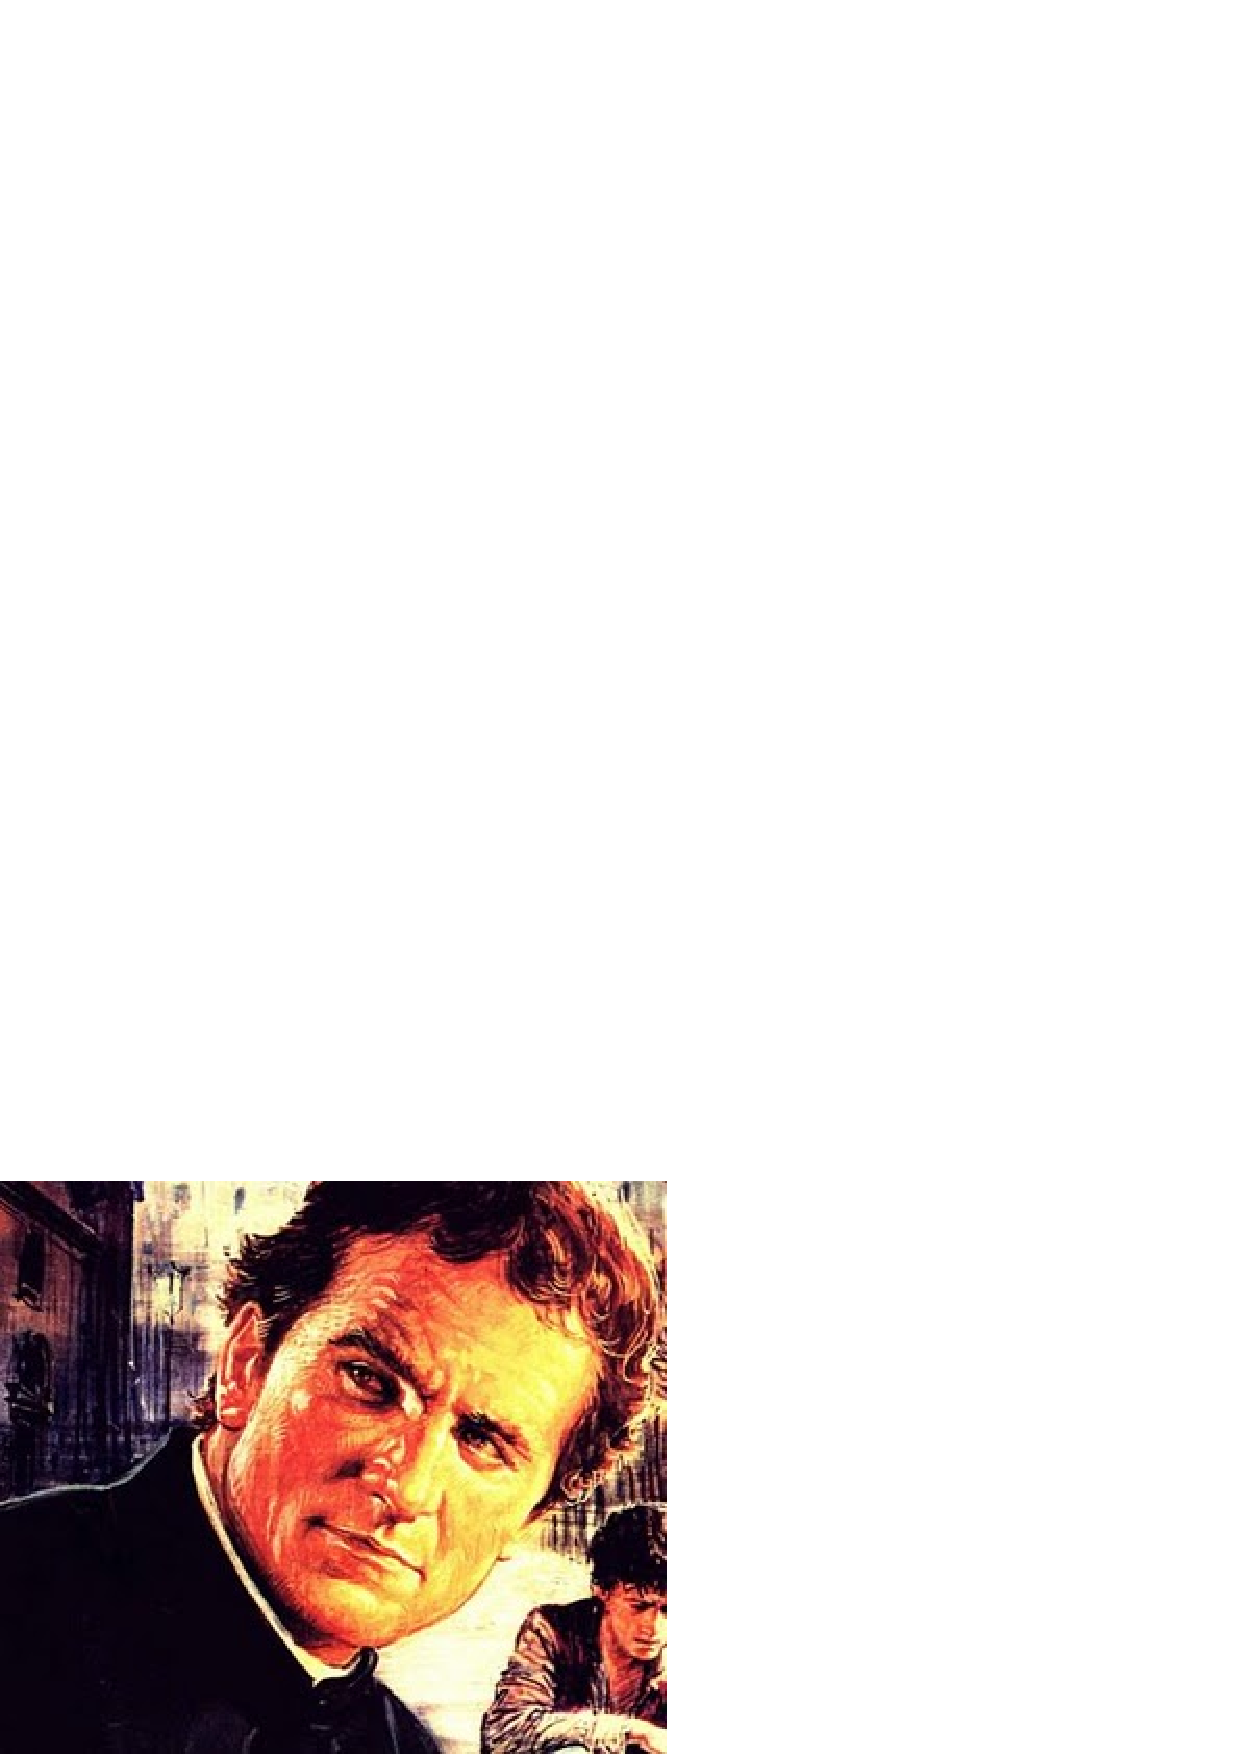
\includegraphics[scale=0.5]{images/san-juan-bosco}
	\caption{San Juan Bosco, patrono de los jóvenes}
	\label{fig:don-bosco}
\end{figure}

Con motivo del 150 aniversario de la fundación de la Congregación de San Francisco de Sales (25 de abril de 2010) y del 200 aniversario del nacimiento del santo (1815-2015), las reliquias de Don Bosco visitan las comunidades de todo el mundo. En México, la gira inició el 4 de agosto en la Ciudad de México y concluyó el 11 de septiembre en Tijuana, B.C.N.; estuvo en Irapuato el 23 de agosto en una velada que atrajo a 5 mil personas.

En todas las poblaciones que estuvo la concurrencia fue nutrida, despertando expectación y curiosidad por conocer su vida y obra; se piensa aprovechar la sensibilización de la comunidad local para difundir información sobre el patrono de los jóvenes.

Algunos rasgos de su personalidad y su obra son:

\begin{itemize}
	\item Se le veía siempre rodeado de muchachos en un ambiente festivo, con música, risas y entusiasmo; conquistó el corazón de los jóvenes para educarlos.
	\item Instaló en sus escuelas diversos talleres (zapatería, sastrería, carpintería, imprenta) para preparar a los jóvenes para un trabajo digno.
	\item Confiaba en las persona y sabía ganarse su confianza, en una ocasión salió de paseo con los presos de la ciudad de Turín sin guardia alguno, al volver no escapó ninguno.
	\item Caminaba en la cuerda floja, realizaba malabares y trucos de magia, es patrono de los ilusionistas.
	\item Hospedaba huérfanos y les daba educación.
	\item Procuró mejorar las condiciones de trabajo de sus jóvenes y cuando no pudo convencer a sus patrones, él mismo les dio trabajo instalando talleres e imprenta.
\end{itemize}

Aplicado a la institución, significa considerar las notas señaladas en la sección \ref{sub:intro:NotasDistintivas} (página \pageref{sub:intro:NotasDistintivas}): \emph{sistema preventivo, acompañamiento, formación en valores, quitar barreras de discriminación, formación para el trabajo}

De este centro se desprenden de forma natural diversas características considerando los perfiles de clientes de la sección \ref{sec:Clientes} (página \pageref{sec:Clientes}) y en respuesta a la oferta de los competidores (cuadro \ref{tbl:CompetidoresDetalle}. p\'agina \pageref{tbl:CompetidoresDetalle}):

\begin{itemize}
	\item
	La preparatoria particular con el programa de becas más extenso, que busca continuamente cómo bajar sus precios para que nadie se quede sin estudiar.
	\item
	Uno de los colegios particulares de calidad con colegiaturas más bajas.
	\item
	Incorporada a la red de escuelas salesianas con todo el prestigio que implica.
	\item
	Atención y acompañamiento personalizados con base en el sistema preventivo.
	\item
	Uno de los pocos bachilleratos con carrera técnica, que capacita para el trabajo, para que el egresado pueda sostener sus estudios universitarios trabajando a tiempo parcial o si lo decide, incorporarse al medio laboral.
	\item
	La escuela tiene un fuerte compromiso en transmitir los valores cristianos y humanos formando <<Buenos Cristianos y Honestos Ciudadanos>> capaces de asumir compromisos con su familia y comunidad.
	\item
	El bachillerato tiene programas de vinculación empresarial con lo que permite la posibilidad de conseguir empleo a tiempo parcial o completo, conocer la industria y saber que la carrera técnica elegida corresponde con las necesidades laborales del mundo real.
\end{itemize}

\section{Promoción}

La promoción abarca cinco estrategias fundamentales, cada una de las cuales combina diversos instrumentos, se enfoca en determinados espacios y/o lugares, participan distintos agentes y persiguen objetivos precisos.

Los objetivos de la promoción son:

\begin{itemize}
	\item Interesar a los egresados de secundaria en ingresar al bachillerato tecnológico.
	\item Dar a conocer entre los vecinos, principalmente de los barrios populares, la nueva escuela como opción de superación.
	\item Dar a conocer al público en general la vida y obra de Don Bosco, su sistema educativo preventivo y la preparatoria que lo llevará a cabo en Irapuato.
	\item Llegar al público joven a través de Internet.
	\item Proporcionar informes y orientación.
\end{itemize}

Para lograrlo se tienen las siguientes cinco estrategias:

\begin{description}
	\item[Campaña de orientación vocacional en secundarias] visitas, conferencias, videos, carteles.
	\item[Campaña educativa en la calle] carteles en comercios, casas de la cultura, iglesias, mamparas en espacios públicos, etc. Volanteo en los barrios. Acceder a las comunidades de vecinos a través de la Iglesia en las misas, mediante grupos juveniles, aprovechando el apoyo de los párrocos, etc.
	\item[Promoción abierta] participación en programas de radio y televisión local, artículos y anuncios en el periódico, publicidad en espectaculares, etc.
	\item[Campaña por Internet] creación de sitio web, blog y cuentas en redes sociales (Facebook y Twitter). Elaboración de presentaciones electrónicas y colocación de videos en YouTube.
	\item[Centro telefónico] para proporcionar informes y orientación.
\end{description}

Las cinco estrategias se basan en la conformación de una red social integrada por miembros de la comunidad salesiana, ex-alumnos salesianos y voluntarios.

\section{Precio}

El precio base es de \$ 3,000.00. Sobre el precio existen diferentes estrategias:

\begin{itemize}
	\item Descuento por pago puntual
	\item Beca por aprovechamiento
	\item Beca por situación socioeconómica
	\item Beca por varios miembros de familia
	\item El porcentaje del monto asignado a becas se incrementa a medida que la matrícula crece
	\item Las becas se incrementan en la medida de los patrocinios que se obtengan
	\item Precio especial para hijos de trabajadores de empresas patrocinadoras
\end{itemize}


\chapter{Administración de Operaciones}

\section{Plan de Inicio}
\label{sec:Plan:Inicio}

A continuación se describe el plan de inicio, de los nueve aspectos de la planeación señalados por el Project Management Institute \citep{PMBOK2008} se destacan cinco por considerarse los más relevantes para el presente trabajo:

\begin{description}
	\item [Alcance]  Las tareas y resultados que se deben obtener, así como su interdependencia.
	\item [Tiempo]   El tiempo que tomará realizar el alcance y la distribución de las tareas en el calendario.
	\item [Costo]    El costo asociado al logro de los resultados.
	\item [Insumos]  Los materiales requeridos para realizar las tareas.
	\item [Personal] Las personas responsables de cada parte del alcance
\end{description}

El detalle del plan se puede apreciar en los cuadros \ref{tbl:Proy:Gantt}, \ref{tbl:Proy:Costos}, \ref{tbl:Proy:Personal:Costos} y \ref{tbl:Proy:Insumos}. (Páginas \pageref{tbl:Proy:Gantt}, \pageref{tbl:Proy:Costos}, \pageref{tbl:Proy:Personal:Costos} y \pageref{tbl:Proy:Insumos} respectivamente); se consideró un enfoque basado en esfuerzo (horas/hombre) para todas las tareas excepto aquellas que demandaban una cobertura de tiempo\footnote{Se utilizó la herramienta TaskJuggler para la programación y cómputo de los tiempos y costos (\texttt{http://www.taskjuggler.org/})}.

Conviene hacer una aclaración sobre el estimado del proyecto: los datos obtenidos se consideran provisionales, una vez que se integre el \emph{staff} del proyecto, se delegará a cada responsable la programación detallada de su encargo y se reestimarán tiempos y costos.\label{sec:Proy:Aclaracion}

\subsection{Alcance}

Para que la escuela inicie sus operaciones exitosamente se requiere lograr los siguientes resultados:

\begin{itemize}
	\item Conformación del Patronato
	\item Procesos internos y reglamento elaborados
	\item Infraestructura, instalaciones. servicios y mobiliario listos
	\item Material didáctico disponible
	\item Personal contratado y capacitado
	\item Planes y programas de estudio elaborados
	\item Permisos y trámites realizados
	\item Promoción realizada
	\item Patrocinios y enlaces empresariales listos
\end{itemize}

\subsection{Tiempo}

Las actividades para iniciar el bachillerato tienen una duración de 7,280 horas, comenzando el 1º de diciembre de 2010 y terminando el 18 de julio  de 2011.

\subsection{Costo}
\label{sub:Proy:Costo}

El costo está asociado directamente con los insumos y el tiempo que cada persona dedica al proyecto (sueldos y honorarios). Iniciar este proyecto demanda \$~2,757,975.00; de los cuales, \$~1,806,300.00 corresponden a insumos y \$~951,675.00 a sueldos y honorarios del \emph{staff} del proyecto.

\subsection{Insumos}

Los insumos se detallan en el cuadro \ref{tbl:Proy:Insumos} (página \pageref{tbl:Proy:Insumos}). Se dividen en tres grupos: infraestructura, mobiliario y equipamiento (talleres y salas de cómputo).

Por infraestructura se requiere invertir \$~197,300.00, el costo del mobiliario es de \$~509,000.00 y para equipamiento se consideraron \$~1,100,000.00.

\subsection{Personal}

El \emph{staff} requerido para iniciar el proyecto está conformado por 15 personas cubriendo los siguientes roles (cuadro \ref{tbl:Proy:Personal:Costos}):

\begin{itemize}
	\item Patrocinador (una persona)
	\item Relaciones Públicas (cuatro personas)
	\item Líder de Proyecto (una persona)
	\item Infraestructura\footnote{Responsable de dar seguimiento a los servicios de remodelación contratados, gestionar las compras y la instalación del mobiliario por parte del proveedor} (una persona)
	\item Docencia y Pastoral (tres personas)
	\item Capital Humano (tres personas)
	\item Asuntos legales (una persona)
\end{itemize}

\clearpage

\begin{table}
    \centering
    \caption{Diagrama de Gantt$^{/a}$ del Inicio del Proyecto}
    \label{tbl:Proy:Gantt}
    \footnotesize
    \begin{tabular}{r|p{6cm}|c|c|c|c|c|c|c|c}
        \multicolumn{2}{c|}{TAREA}                                         & DIC & ENE & FEB & MAR & ABR & MAY & JUN & JUL \\
        \hline
        \hline
        \multicolumn{2}{l|}{Inicio del Proyecto}                           & XXX & XXX & XXX & XXX & XXX & XXX & XXX & XXX \\
        \hline
        1  & Obtener Aprobación de la Inspectoría                          & XXX &     &     &     &     &     &     &     \\
        2  & Administración del proyecto                                   & XXX &     &     &     &     &     &     &     \\
        3  & Conformación del Patronato                                    &     & XXX & XXX & XXX &     &     &     &     \\
        3  & Procesos Internos y Reglamento Elaborados                     &     &     &     &     & XXX & XXX &     &     \\
        4  & Permisos y Trámites Realizados                                &     & XXX & XXX &     &     &     &     &     \\
        5  & Planes y Programas de Estudio Elaborados                      &     & XXX & XXX &     &     &     &     &     \\
        6  & Material Didáctico Disponible                                 &     &     & XXX & XXX &     &     &     &     \\
        7  & Infraestructura, Instalaciones, Servicios y Mobiliario Listos &     & XXX & XXX & XXX & XXX & XXX &     &     \\
        8  & Promoción realizada                                           &     & XXX & XXX & XXX & XXX & XXX & XXX & XXX \\
        9  & Patrocinios y enlaces empresariales listos                    &     & XXX & XXX & XXX & XXX & XXX & XXX & XXX \\
        10 & Personal Contratado y Capacitado                              &     &     & XXX & XXX & XXX &     &     &     \\
        \hline
        \multicolumn{10}{l}{\footnotesize Fuente: Elaboración Propia, 2010.} \\
        \multicolumn{10}{l}{$^{/a}$ \footnotesize Más información sobre el diagrama de Gantt en \citep{PMBOK2008}.}
    \end{tabular}
\end{table}



\begin{table}
    \centering
    \caption{Costos del Proyecto por Tarea}
    \label{tbl:Proy:Costos}
    \footnotesize
    \begin{tabular}{r|l|r|r}
        \multicolumn{2}{c|}{TAREA}                                         & COSTO   & ESFUERZO \\ 
        \hline
        \hline
        \multicolumn{2}{l|}{Inicio del Proyecto}                           & 951,675 & 7,280    \\ 
        \hline
         1 & Obtener Aprobación de la Inspector\'ia                        & 0       & 0        \\ 
         2 & Administraci\'on del proyecto                                 & 153,000 & 1,208    \\ 
         3 & Conformación del Patronato                                    & 18,750  & 100      \\ 
         4 & Procesos Internos y Reglamento Elaborados                     & 11,250  & 60       \\ 
         5 & Permisos y Tr\'amites Realizados                              & 18,750  & 150      \\ 
         6 & Planes y Programas de Estudio Elaborados                      & 35,300  & 301      \\ 
         7 & Material Did\'actico Disponible                               & 35,475  & 302      \\ 
         8 & Infraestructura, Instalaciones, Servicios y Mobiliario Listos & 93,250  & 746      \\ 
         9 & Patrocinios y enlaces empresariales listos                    & 31,950  & 220      \\ 
        10 & Promoci\'on realizada                                         & 439,650 & 3,029    \\ 
        11 & Personal Contratado y Capacitado                              & 108,675 & 1,134    \\ 
        \hline
        \multicolumn{4}{l}{\footnotesize Fuente: Elaboración Propia, 2010.}
    \end{tabular}
\end{table}


\begin{table}
    \centering
    \caption{\emph{Staff} del Proyecto con Sueldos por Hora}
    \label{tbl:Proy:Personal:Costos}
    \footnotesize
    \begin{tabular}{l|r}
        \multicolumn{1}{c|}{NOMBRE}                     & \multicolumn{1}{c}{SUELDO/HR} \\
        \hline
        \hline
        \multicolumn{2}{l}{Patrocinador}                                                \\
        \hline
        \hspace{1em} Pbro. Edmundo Morales              & \$ 187.50                     \\
        \hline
        \multicolumn{2}{l}{Administración Proyectos}                                    \\
        \hline
        \hspace{1em} Gustavo Serrano Diez               & \$ 125.00                     \\
        \hline
        \multicolumn{2}{l}{Relaciones Publicas}                                         \\
        \hline
        \hspace{1em} Miguel Ayala Ortiz                 & \$ 150.00                     \\
        \hspace{1em} Auxiliar Relaciones Públicas 1     & \$ 100.00                     \\
        \hspace{1em} Auxiliar Relaciones Públicas 2     & \$ 100.00                     \\
        \hspace{1em} Auxiliar Relaciones Públicas 3     & \$ 100.00                     \\
        \hline
        \multicolumn{2}{l}{Infraestructura}                                             \\
        \hline
        \hspace{1em} Responsable de Infraestructura     & \$ 125.00                     \\
        \hline
        \multicolumn{2}{l}{Docencia y Pastoral}                                         \\
        \hline
        \hspace{1em} Responsable de Docencia y Pastoral & \$ 125.00                     \\
        \hspace{1em} Auxiliar de Docencia y Pastoral 1  & \$ 100.00                     \\
        \hspace{1em} Auxiliar de Docencia y Pastoral 2  & \$  62.50                     \\
        \hline
        \multicolumn{2}{l}{Capital Humano}                                              \\
        \hline
        \hspace{1em} Responsable de Capital Humano      & \$ 125.00                     \\
        \hspace{1em} Auxiliar Capital Humano 1          & \$ 100.00                     \\
        \hspace{1em} Auxiliar Capital Humano 2          & \$  62.50                     \\
        \hline
        \multicolumn{2}{l}{Asuntos Legales}                                             \\
        \hline
        \hspace{1em} Abogado                            & \$ 125.00                     \\
        \hline
        \multicolumn{2}{l}{\footnotesize Fuente: Elaboración Propia, 2010.}
    \end{tabular}
\end{table}


\begin{table}
    \centering
    \caption{Costos de los Insumos}
    \label{tbl:Proy:Insumos}
    \footnotesize
    \begin{tabular}{c|l|r}
      & \multicolumn{1}{c|}{ELEMENTO}    & \multicolumn{1}{c}{COSTO} \\
        \hline
        \hline
        \multirow{8}{*}{INFRAESTRUCTURA} &
        Pintura                          & \$ 66,800.00              \\
      & Resanamiento                     & \$ 40,000.00              \\
      & Herrería                         & \$ 15,000.00              \\
      & Cerrajería                       & \$ 7,500.00               \\
      & Impermeabilización               & \$ 48,000.00              \\
      & Plomería                         & \$ 5,000.00               \\
      & Electricidad                     & \$ 15,000.00              \\
        \cline{2-3}
      & Total                            & \$ 197,300.00             \\
        \hline
        \multirow{10}{*}{MOBILIARIO}     &
        Pizarrones                       & \$ 100,000.00             \\
      & Pupitres                         & \$ 360,000.00             \\
      & Escritorios oficina              & \$ 25,000.00              \\
      & Sillas oficina                   & \$ 5,000.00               \\
      & Material conserjería             & \$ 3,500.00               \\
      & Plumones                         & \$ 2,000.00               \\
      & Borradores                       & \$ 500.00                 \\
      & Mesa sala de juntas              & \$ 10,000.00              \\
      & Sillas sala de juntas            & \$ 3,000.00               \\
        \cline{2-3}
      & Total                            & \$ 509,000.00             \\
        \hline
        \multirow{3}{*}{EQUIPAMIENTO}    &
        Equipo para talleres             & \$ 500,000.00             \\
      & Computadoras                     & \$ 600,000.00             \\
        \cline{2-3}
      & Total                            & \$ 1,100,000.00           \\
        \hline
        \hline
        \multicolumn{2}{r|}{Total}       & \$ 1,806,300.00           \\
        \hline
        \multicolumn{3}{l}{\footnotesize Fuente: Elaboración Propia, 2010.}
    \end{tabular}
\end{table}


\clearpage

\section{Plan de Operaciones}

El plan de operaciones surge de la exploración de las actividades más relevantes de la institución, las cuales, a su vez desembocan en la estructura organizacional necesaria para operar.

\subsection{Actividades}

Una enumeración preliminar de las actividades se muestra en el cuadro \ref{tbl:Oper:Actividades}. A modo de lluvia de ideas se obtuvieron las tareas de mayor relevancia para el funcionamiento de la escuela, posteriormente se ordenaron de acuerdo a su periodicidad y a partir de ahí se identificaron las siguientes dos áreas de operación:

\begin{description}
	\item[Actividades de Docencia]
		Todas aquellas relacionadas directamente con el proceso de enseñanza-aprendizaje de los jóvenes.
	\item[Actividades Administrativas]
		Son las relativas al sostenimiento y funcionamiento del bachillerato en cuanto organización humana.
\end{description}

Se tiene programado un mapeo a fondo de los procesos internos de la institución como puede observarse en el cuadro \ref{tbl:Proy:Gantt} (página \pageref{tbl:Proy:Gantt})\footnote{Considérese la aclaración sobre la provisionalidad de las fechas y detalles del plan de inicio como se indica en la página \pageref{sec:Proy:Aclaracion}}.

\begin{table}
    \centering
    \caption{Plan de Operaciones: Actividades por Periodo}
    \label{tbl:Oper:Actividades}
    \footnotesize
    \begin{tabular}{l|p{0.8\textwidth}}
        \multicolumn{2}{c}{ACTIVIDAD A DIARIO} \\ 
        \hline
        \hline
        Docencia &
        Control de asistencia. Impartir clases. Actividades en recreo. Confesiones y comuniones en capilla. Acompañamiento alumnos. Control de salidas y permisos. Cuidar buen comportamiento. Resolver problemas con alumnos y profesores. \\ 
        \hline
        Administración &
        Abrir puerta y salones. Registrar entrada de personal. Entrada de estudiantes con credencial. Registrar visitantes. Entregar plumones, borradores y proyectores. Recibir llamadas. Atender padres de familia, alumnos, profesores, autoridades y visitantes. Seguimiento a patrocinadores. Búsqueda de patrocinadores. Soporte técnico equipos de cómputo. Limpieza. Registrar salida. Parte diario. Cierre de salones y puerta. \\
        \hline
        \multicolumn{2}{c}{ACTIVIDAD SEMANAL} \\ 
        \hline
        \hline
        Docencia &
        Oración comunitaria. Sesiones de grupos apostólicos. Revisar avance de grupo. Jornadas de servicio. Seguimiento a profesores. \\ 
        \hline
        Administración &
        Actualizar página Web. Surtir material de papelería, limpieza, sanitarios. Revisar existencias en bodegas. Parte semanal. \\
        \hline
        \multicolumn{2}{c}{ACTIVIDAD MENSUAL} \\ 
        \hline
        \hline
        Docencia &
        Honores a la bandera. Entrevistar alumnos. Misa comunitaria. \\ 
        \hline
        Administración &
        Recibir comprobantes pago colegiaturas. Aplicar patrocinio a becas. Renta a papelería. Renta a comedor. Resurtir borradores y plumones. Adquirir material talleres. Pago servicios telecomunicaciones. Pago limpieza. Pago vigilancia. Pago de nómina y honorarios. Pago despacho contable. Pago de impuestos. Declaraciones parciales. Corte de caja. Reporte mensual. \\
        \hline
        \multicolumn{2}{c}{ACTIVIDAD BIMESTRAL} \\ 
        \hline
        \hline
        Docencia &
        Exámenes parciales. Publicación calificaciones. Junta padres de familia. Evaluación avance de cursos. Imprimir listas de alumnos. Boletín salesiano. Obra de teatro. Evaluación pastoral. Simulacro protección civil. Eventos y ferias temáticas. Reunión consejo escolar y sociedad de alumnos. Acompañamiento a profesores. \\ 
        \hline
        Administración &
        Monitoreo becas. Mantenimiento preventivo equipos de cómputo. Surtir enfermería. Pagar agua, luz y predial. Reporte bimestral. \\
        \hline
        \multicolumn{2}{c}{ACTIVIDAD SEMESTRAL} \\ 
        \hline
        \hline
        Docencia &
        Conformación de grupos y horarios. Elaboración de planes de clase. Convivencia de inicio de cursos. Visita empresarial. Torneo deportivo. Retiro semestral. Exámenes finales. Evaluación final. Exámenes extraordinarios. Evaluación profesores. Cierre semestral. Cursos intersemestrales. \\ 
        \hline
        Administración &
        Inscripciones. Emisión de credenciales. Asignación de becas. Contrataciones. Inducción. Capacitación profesores. Cobro de inscripciones. Evaluación proveedores. Resurtir equipo deportivo. Informe semestral. \\
        \hline
        \multicolumn{2}{c}{ACTIVIDAD ANUAL} \\ 
        \hline
        \hline
        Docencia &
        Campamento. Peregrinación al Cubilete. Elecciones sociedad de alumnos. Premiaciones. Visita a secundarias. \\ 
        \hline
        Administración &
        Ajustes a estrategia. Trámite de cédulas y certificados. Ajuste salarial. Contratos de servicios. Reemplazo de mobiliario dañado. Resurtir biblioteca. Programa de remodelaciones. Seleccionar proveedores. Pago de aguinaldos. Declaración anual. Auditoría externa. Resurtir laboratorios y talleres. Campaña de patrocinios. Campaña de promoción. Informe anual. \\
        \hline
        \multicolumn{2}{c}{ACTIVIDAD CADA CINCO AÑOS} \\ 
        \hline
        \hline
        Administración &
        Plan estratégico. Expansión. Reemplazo equipos de cómputo. Reemplazo maquinaria talleres. Reemplazo de mobiliario. \\
        \hline
        \multicolumn{2}{l}{\footnotesize Fuente: Elaboración Propia, 2010.}
    \end{tabular}
\end{table}

\clearpage

\subsection{Estructura Organizacional}

La estructura organizacional del bachillerato se considera desde dos ángulos diferentes: estructura funcional de puestos de trabajo y órganos de representación.

\subsubsection{Estructura Funcional}

Funcionalmente, las actividades de la escuela pueden clasificarse en cuatro rubros: a) docencia, b) pastoral, c) administración y d) relaciones públicas. El rubro con más personal a su cargo es el de docencia, pues incluye a todos los profesores. Se propone un coordinador por cada carrera técnica que se abra. El organigrama final completo puede observarse en la figura \ref{fig:Org:Final}.

%La escuela divide sus actividades en dos grandes grupos funcionales: docencia y administración, mostrados en las figuras \ref{fig:Org:Docencia} y \ref{fig:Org:Administracion}; un director general es el vínculo entre ambase estructuras, las cuales consideran a la institución en un estado de desarrollo ya maduro y con la matrícula suficiente (más del 50\% de la capacidad instalada).

Para iniciar operaciones se tiene un organigrama inicial mostrado en la figura \ref{fig:Org:Inicial}; el cual parte del \emph{staff} de inicio del proyecto e irá evolucionando hasta el organigrama final mediante la delegación paulatina de responsabilidades en personal a cargo.

De igual forma, los sueldos en los cargos jerárquicos se incrementarán a medida que incrementa el alumnado; esta medida que inicialmente es de ahorro ante un escenario pesimista, constituye al mismo tiempo un aliciente para lograr el mayor éxito de la escuela (ver el cuadro \ref{tbl:Org:Sueldos} de la página \pageref{tbl:Org:Sueldos}).

Los sueldos propuestos se basan en los siguientes criterios: para el profesorado y niveles jerárquicos bajos el retribuir justamente un trabajo frecuentemente minusvalorado. Para los niveles jerárquicos de autoridad: resolver la tensión que por un lado produce la necesidad de contar con personas altamente capaces y comprometidas; y por otra parte, la práctica de austeridad que acerque a los directivos a aquellos a quienes desean beneficiar y servir: los pobres.

\begin{figure}
	\centering
	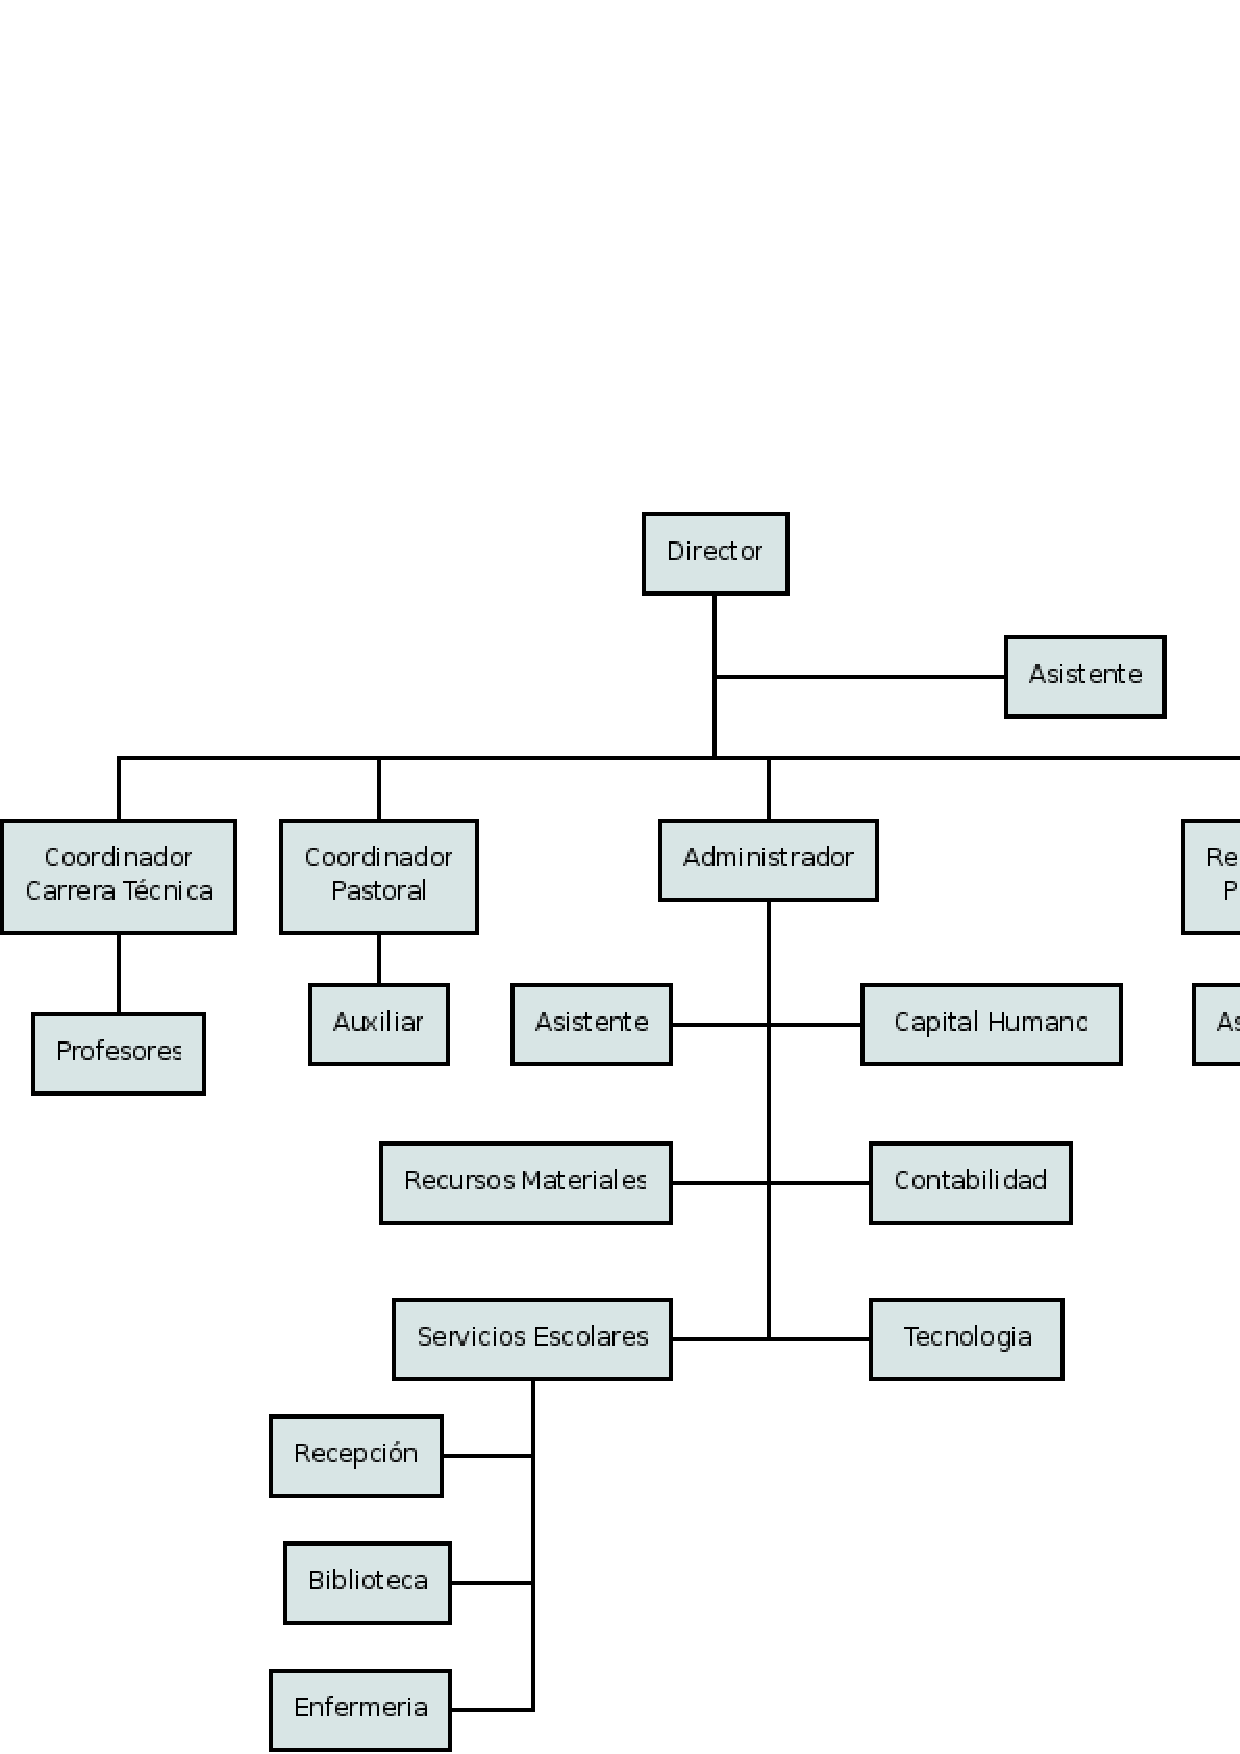
\includegraphics[scale=0.7]{images/organigrama-final}
	\caption{Organigrama Final. Fuente: Elaboración Propia.}
	\label{fig:Org:Final}
\end{figure}

\begin{figure}
	\centering
	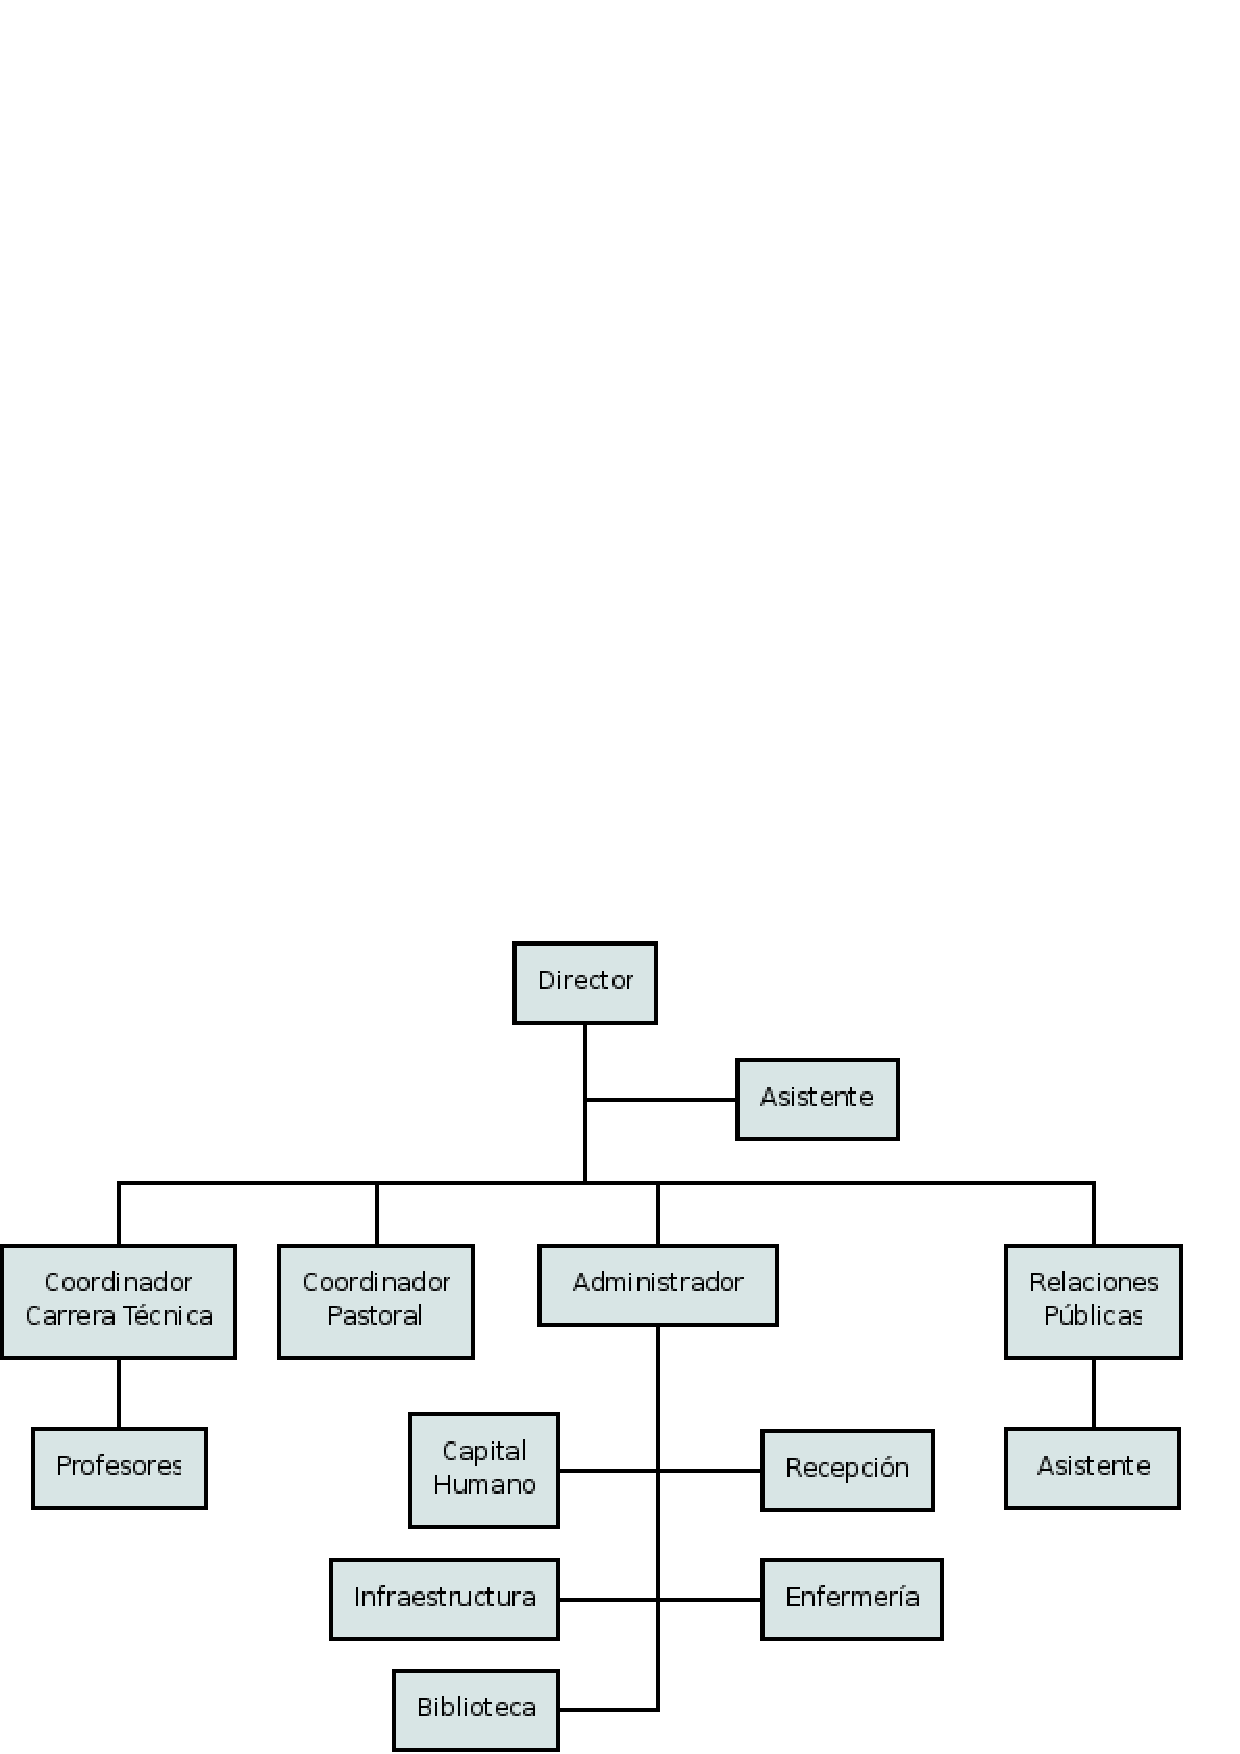
\includegraphics[scale=0.7]{images/organigrama-inicial}
	\caption{Organigrama Inicial. Fuente: Elaboración Propia.}
	\label{fig:Org:Inicial}
\end{figure}

\begin{table}[h]
    \centering
    \caption{Tabla de Sueldos por Cargo}
    \label{tbl:Org:Sueldos}
    \footnotesize
    \begin{tabular}{l|c|c|r|r}
                & \multicolumn{1}{c|}{CANTIDAD}
                & \multicolumn{1}{c|}{CANTIDAD}
                & \multicolumn{1}{c|}{SUELDO}
                & \multicolumn{1}{c}{SUELDO} \\
        \multicolumn{1}{c|}{CARGO}
                & \multicolumn{1}{c|}{INICIAL}
                & \multicolumn{1}{c|}{FINAL}
                & \multicolumn{1}{c|}{INICIAL$^{/a}$}
                & \multicolumn{1}{c}{MENSUAL$^{/b}$} \\
        \hline
        \hline
        Director General                 & 1 &  1 & \$ 21,000.00 & \$ 30,000.00 \\
        Coordinador de Carrera Técnica   & 1 &  3 & \$ 17,500.00 & \$ 25,000.00 \\
        Coordinador de Pastoral          & 1 &  1 & \$ 17,500.00 & \$ 25,000.00 \\
        Administrador                    & 1 &  1 & \$ 17,500.00 & \$ 25,000.00 \\
        Relaciones Públicas              & 1 &  1 & \$ 17,500.00 & \$ 25,000.00 \\
        Encargado de Capital Humano      & 1 &  1 & \$ 14,000.00 & \$ 20,000.00 \\
        Encargado de Infraestructura     & 1 &  0 & \$ 14,000.00 &  N/A$^{/c}$  \\
        Encargado de Contabilidad        & 0 &  1 &       N/A    & \$ 20,000.00 \\
        Encargado de Tecnología          & 0 &  1 &       N/A    & \$ 20,000.00 \\
        Encargado de Recursos Materiales & 0 &  1 &       N/A    & \$ 20,000.00 \\
        Encargado de Servicios Escolares & 0 &  1 &       N/A    & \$ 20,000.00 \\
        Asistente de Dirección           & 2 &  3 & \$ 15,000.00 & \$ 15,000.00 \\
        Enfermera                        & 1 &  1 & \$ 15,000.00 & \$ 15,000.00 \\
        Profesor$^{/d}$                  & 8 & 34 & \$ 16,800.00 & \$ 16,800.00 \\
        Auxiliar                         & 0 &  1 & \$ 10,000.00 & \$ 10,000.00 \\
        Biblioteca                       & 1 &  1 & \$  9,000.00 & \$  9,000.00 \\
        Recepcionista                    & 1 &  1 & \$  9,000.00 & \$  9,000.00 \\
        \hline
        \multicolumn{5}{l}{\footnotesize Fuente: Elaboración Propia, 2010.} \\
        \multicolumn{5}{p{5.5in}}{$^{/a}$ 30\% menor con respecto al definitivo durante los primeros dos años} \\
        \multicolumn{5}{p{5.5in}}{$^{/b}$ Calculado en 2010, se considera 2.5\% de inflación anual} \\
        \multicolumn{5}{p{5.5in}}{$^{/c}$ N/A significa que el puesto no se considera en en escenario indicado} \\
        \multicolumn{5}{p{5.5in}}{$^{/d}$ El sueldo de un profesor es de \$120.00 la hora, la cantidad de \$16.800.00 se calcula sobre la base de que un grupo recibe 35 horas de clase a la semana. Las cantidades indicadas de 8 y 34 corresponden al número de grupos}
    \end{tabular}
\end{table}

\clearpage

\subsubsection{Órganos de Representación}

La escuela cuenta con los siguientes órganos de representación:

\begin{description}
	\item[Patronato]
		Es la máxima autoridad de la escuela, a este órgano rinde cuentas el director por los resultados obtenidos. Tiene un presidente a la cabeza, el cual será siempre un miembro de la congregación salesiana.
	\item[Consejo Escolar]
		Se reúnen con el propósito de proponer mejoras a la escuela tanto académicas como estratégicas. A partir de esta información se mejorará el plan estratégico de la institución. El presidente es el director.
	\item[Sociedad de Alumnos]
		Tiene como finalidad representar a los estudiantes ante el consejo escolar, además de realizar diversas tareas de servicio en coordinación con el alumnado. Tiene un presidente y una planilla que son electos por sus compañeros una vez al año.
\end{description}

\begin{figure}[h]
	\centering
	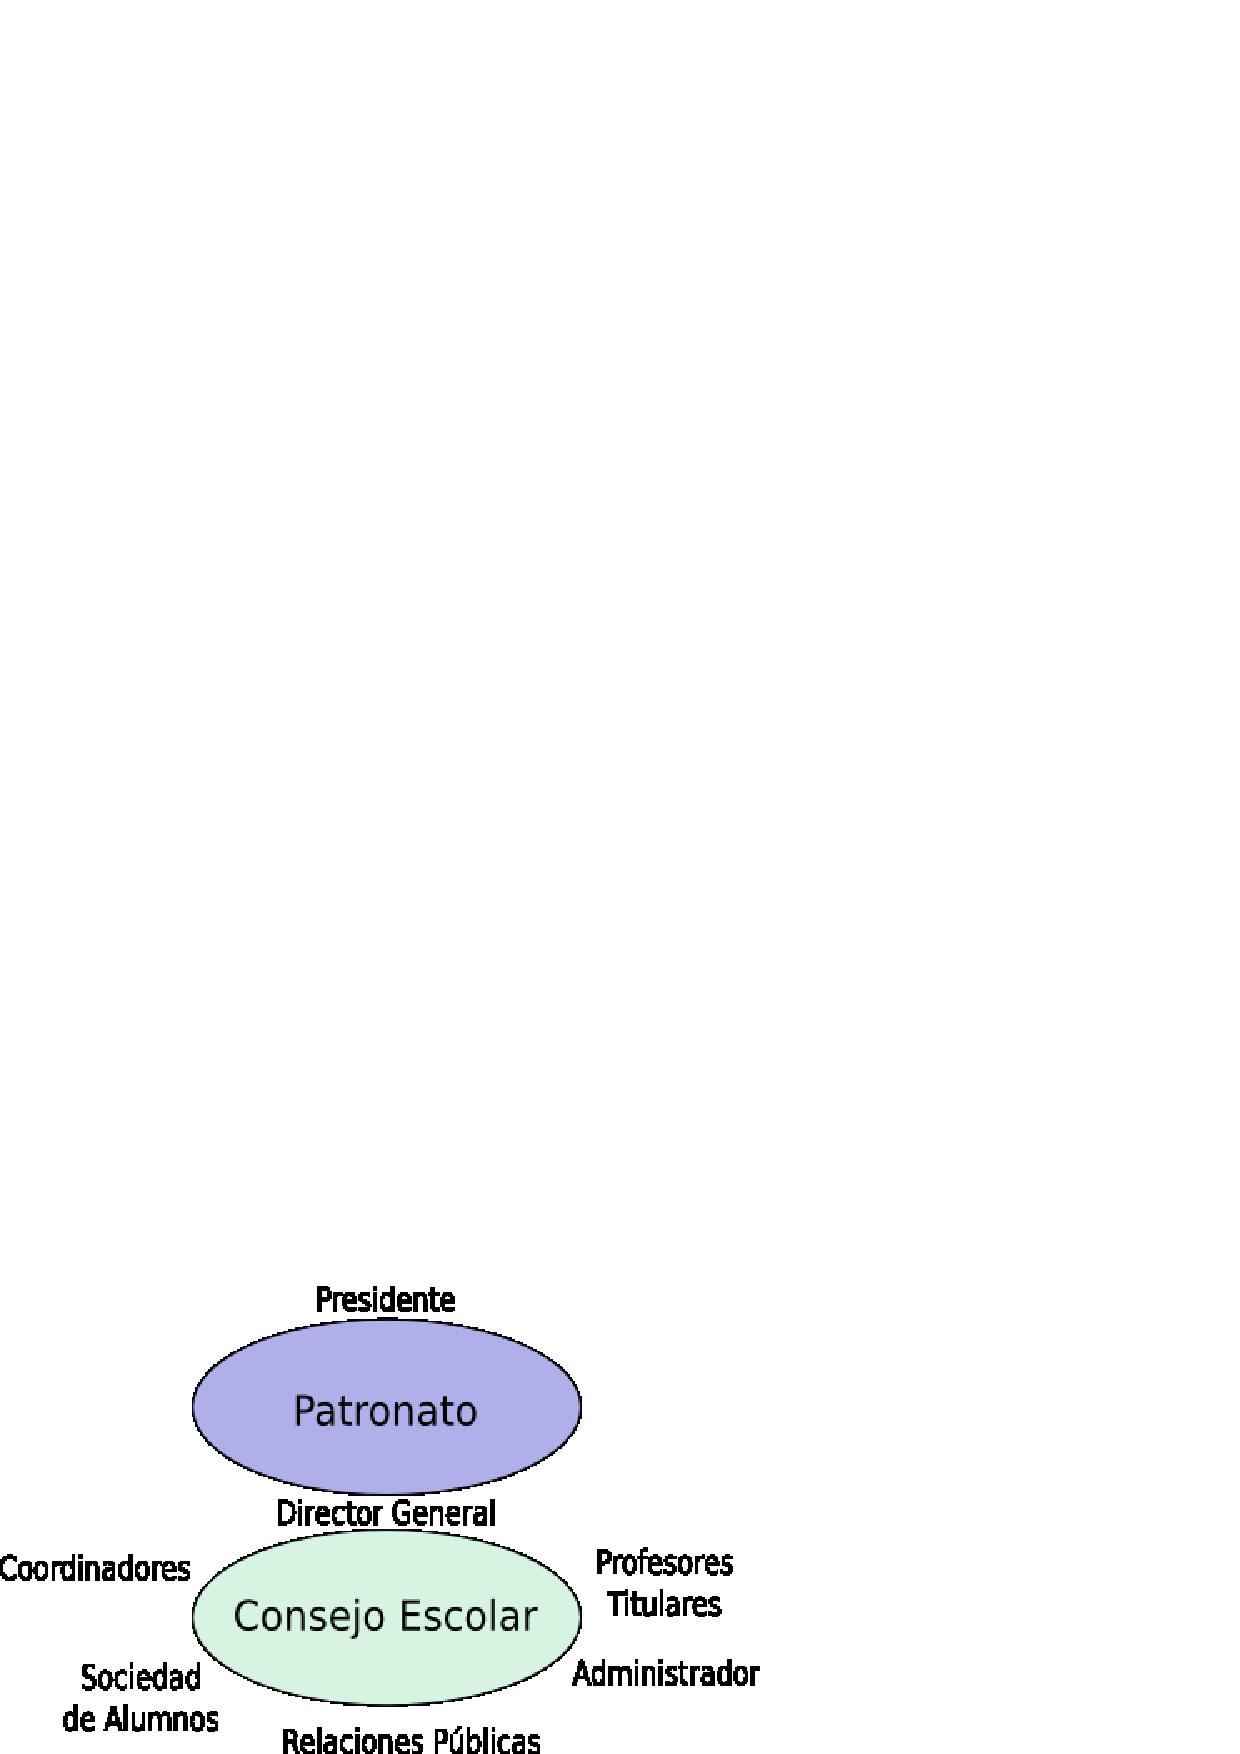
\includegraphics{images/organos}
	\caption{Órganos de Representación. Fuente: Elaboración Propia.}
	\label{fig:Org:Organos}
\end{figure}
\clearpage

\section{Aspectos Contables y Legales}

Se consideran dos figuras legales para la constitución de la escuela, en una primera etapa se trata de una Institución de Asistencia Privada (I.A.P.) ya existente: Vida y Esperanza de México, I.A.P.\footnote{\texttt{http://www.enlace.df.gob.mx/busqueda/consultaOsc2.html?b=V}}; la segunda etapa será constituir una Asociación Civil (A.C.) específica para el bachillerato.

La razón de contemplar ambas opciones es la siguiente: la I.A.P. ya existe y goza de prestigio; permite comenzar la labor. La A.C. le dará mayor independencia a la escuela, sin embargo, el reconocimiento oficial toma más de un año.

\subsection{Consideraciones Generales}

La comunidad salesiana en Irapuato, cuenta actualmente con el apoyo de un despacho contable y legal para el cumplimiento de sus obligaciones, especialmente de la fundación Vida y Esperanza de México, I.A.P.; este mismo despacho brindará sus servicios a la escuela en el área de su competencia.

Como parte de los servicios prestados por el despacho, se contemplan las declaraciones fiscales mensuales y anuales. Apoyo durante las auditorías; revisión de contratos laborales y de servicios, litigios, entre otros.

Se consideran los aspectos legales desde dos niveles: federal y local. En el ámbito federal, lo más importante es la autorización de la SEP. El Reconocimiento de Estudios por parte de la autoridad educativa se piensa obtener mediante la figura de extensión de los bachilleratos tecnológicos ya incorporados ante la SEP por parte de otros colegios salesianos.

En el ámbito local, el aspecto más importante a cubrir es el de protección civil. El requisito es tener a una persona que asista a las capacitaciones y después transmita este conocimiento, a la par que se realizan simulacros y se colocan los señalamientos.

\subsection{Vida y Esperanza de México, I.A.P.}

Esta Fundación existe desde hace varios años, cuenta con la autorización de la Secretaría de Hacienda y Crédito Público (S.H.C.P.) para recibir donativos y extender recibos deducibles de impuestos, tiene por objeto social la educación y es presidida por el Pbro. Edmundo Morales Romero, S.D.B.

La principal obligación de la I.A.P. consiste en que cada año es auditada externamente.

\subsection{Una A.C. para el Bachillerato Tecnológico}

Con el propósito de darle independencia legal y financiera a la institución, se tiene pensado crear una A.C. específica; el trámite ante la S.H.C.P. toma de uno a dos años.

En términos generales, una I.A.P. está más acotada por la ley en cuanto a sus funciones y tiene mayor intervención gubernamental tanto en su constitución como en su operación.

Las principales obligaciones de una A.C. son llevar los registros contables y presentar declaraciones mensuales y anuales.

\section{Costos}
\label{sec:Costos}

En una institución educativa, el costo más importante está en los sueldos y salarios; en particular, la nómina de profesores es directamente proporcional al número de estudiantes. Siendo, para este caso, 35 horas por grupo de 30 estudiantes.

La estructura organizacional también aumenta para garantizar el buen orden de las actividades y la coordinación de todos los integrantes de la comunidad.

Para efectos de simplicidad se consideró un profesor de tiempo completo por grupo; sin embargo, en la práctica, la planta docente tiende a ser mucho mayor.

Igualmente, todos los sueldos se colocaron en el rubro de costos fijos, siguiendo el esquema tradicional que se tiene en esta materia.

Como se verá más adelante\footnote{Sección \ref{sec:RecursosColaterales}, página \pageref{sec:RecursosColaterales}.}, se intentará reducir el costo en los diversos rubros mediante patrocinios enfocados.

Un aspecto importante a considerar es la inflación; para este proyecto se consideró de 5\% anual excepto para sueldos, que es de 2.5\% (\citep{BANXICO}).

\subsection{Costos Variables}

Los costos variables están conformados por el material de papelería, didáctico y de talleres. El material de talleres representa la parte más importante. Las carreras técnicas específicas que se impartirán tienen pendiente su definición, por tanto, el costo preciso de materiales y maquinaria también. Esta es la razón por la que los costos se estimaron sobre una base genérica por grupo (cuadro \ref{tbl:Costos:Variables}).

\begin{table}
    \centering
    \caption{Costos Variables}
    \label{tbl:Costos:Variables}
    \scriptsize
    \begin{tabular}{l@{\hspace{1mm}}|r*{5}{|@{\hspace{1mm}}c@{\hspace{1mm}}|@{\hspace{1mm}}r@{\hspace{1mm}}}}
		&	PRECIO	&	\multicolumn{2}{c|}{AÑO 1}	&	\multicolumn{2}{c|}{AÑO 2}	&	\multicolumn{2}{c|}{AÑO 3}	&	\multicolumn{2}{c|}{AÑO 4}	&	\multicolumn{2}{c}{AÑO 5} \\
	\cline{3-12}
	\multicolumn{1}{c|}{CONCEPTO}	&	UNITARIO	&	C$^{/a}$	&	\multicolumn{1}{c|}{TOTAL}	&	C	&	\multicolumn{1}{c|}{TOTAL}	&	C	&	\multicolumn{1}{c|}{TOTAL}	&	C	&	\multicolumn{1}{c|}{TOTAL}	&	C	&	\multicolumn{1}{c}{TOTAL} \\
	\hline
	\hline
	PAPELERÍA \\
	\hline
	Hojas (caja con 5000)	&	200.00	&	4	&	892.00	&	9	&	1,869.00	&	13	&	2,941.47	&	18	&	4,121.15	&	20	&	4,862.03 \\
	Bolígrafos (10 pzas)	&	30.00	&	52	&	1,560.00	&	56	&	1,764.00	&	72	&	2,381.40	&	72	&	2,500.47	&	72	&	2,625.49 \\
	Tóner (2 pzas)	&	2,000.00	&	4	&	8,920.00	&	9	&	18,690.00	&	13	&	29,414.70	&	18	&	41,211.45	&	20	&	48,620.25 \\
	Carpetas (pza.)	&	50.00	&	20	&	1,000.00	&	20	&	1,050.00	&	20	&	1,102.50	&	20	&	1,157.63	&	20	&	1,215.51 \\
	\hline
	SUBTOTAL	&		&		&	12,372.00	&		&	23,373.00	&		&	35,840.07	&		&	48,990.69	&		&	57,323.27 \\
	\hline
	MATERIAL DIDÁCTICO \\
	\hline
	Plumones (4 pzas.)	&	50.00	&	240	&	12,000.00	&	450	&	23,625.00	&	690	&	38,036.25	&	900	&	52,093.13	&	1,020	&	61,990.82 \\
	Borradores (pza.)	&	30.00	&	48	&	1,440.00	&	90	&	2,835.00	&	138	&	4,564.35	&	180	&	6,251.18	&	204	&	7,438.90 \\
	\hline
	SUBTOTAL	&		&		&	13,440.00	&		&	26,460.00	&		&	42,600.60	&		&	58,344.30	&		&	69,429.72 \\
	\hline
	MATERIAL TALLERES \\
	\hline
	Material talleres$^{/b}$	&	5,000.00	&	7	&	35,000.00	&	14	&	73,500.00	&	18	&	99,225.00	&	24	&	138,915.00	&	30	&	182,325.94 \\
	\hline
	SUBTOTAL	&		&		&	35,000.00	&		&	73,500.00	&		&	99,225.00	&		&	138,915.00	&		&	182,325.94 \\
	\hline
	\hline
	TOTAL	&		&		&	60,812.00	&		&	123,333.00	&		&	177,665.67	&		&	246,249.99	&		&	309,078.93 \\
	\hline
	\multicolumn{12}{l}{\footnotesize Fuente: Elaboración Propia, 2010.} \\
	\multicolumn{12}{l}{$^{/a}$ Cantidad} \\
	\multicolumn{12}{l}{$^{/b}$ Material para un grupo de 30 estudiantes} \\
    \end{tabular}
\end{table}


\subsection{Costos Fijos}

El cuadro \ref{tbl:Costos:Fijos} muestra los costos fijos, éstos se integran por los servicios subcontratados (vigilancia, limpieza, etc.), los de infraestructura (agua, luz, etc.), las actividades de promoción (publicidad) y la nómina en sus diferentes niveles.

Para el caso de los servicios subcontratados de vigilancia y limpieza se consideró como unidad el sueldo/mes/hombre. En el caso del despacho contable y legal, una anualidad. Para los servicios de infraestructura (agua, luz, teléfono con internet) se calculó una anualidad mediante la interpolación sobre el estado de resultados de un colegio de menor tamaño en Irapuato\footnote{Uno de los interesados en el proyecto trabaja como administrativo de un bachillerato de pequeño tamaño, fue quien aportó los estados de resultados de su centro de trabajo.}.

\begin{table}
    \centering
    \caption{Costos Fijos}
    \label{tbl:Costos:Fijos}
    \scriptsize
    \begin{tabular}{l@{\hspace{1mm}}|r*{5}{|@{\hspace{1mm}}c@{\hspace{1mm}}|@{\hspace{1mm}}r@{\hspace{1mm}}}}
		&	PRECIO	&	\multicolumn{2}{c|}{AÑO 1}	&	\multicolumn{2}{c|}{AÑO 2}	&	\multicolumn{2}{c|}{AÑO 3}	&	\multicolumn{2}{c|}{AÑO 4}	&	\multicolumn{2}{c}{AÑO 5} \\
	\cline{3-12}
	\multicolumn{1}{c|}{CONCEPTO}	&	UNITARIO	&	C$^{/a}$	&	\multicolumn{1}{c|}{TOTAL}	&	C	&	\multicolumn{1}{c|}{TOTAL}	&	C	&	\multicolumn{1}{c|}{TOTAL}	&	C	&	\multicolumn{1}{c|}{TOTAL}	&	C	&	\multicolumn{1}{c}{TOTAL} \\
	\hline
	\hline
	\multicolumn{12}{l}{SERVICIOS SUBCONTRATADOS} \\
	\hline
	Vigilancia	&	8,000.00	&	72	&	576,000.00	&	72	&	604,800.00	&	72	&	635,040.00	&	72	&	666,792.00	&	72	&	700,131.60 \\
	Limpieza	&	5,000.00	&	40	&	200,000.00	&	40	&	210,000.00	&	40	&	220,500.00	&	40	&	231,525.00	&	40	&	243,101.25 \\
	Despacho legal$^{/b}$	&	60,000.00	&	1	&	60,000.00	&	12	&	756,000.00	&	12	&	793,800.00	&	12	&	833,490.00	&	12	&	875,164.50 \\
	\hline
	SUBTOTAL	&		&		&	836,000.00	&		&	1,570,800.00	&		&	1,649,340.00	&		&	1,731,807.00	&		&	1,818,397.35 \\
	\hline
	\multicolumn{12}{l}{SERVICIOS DE INFRAESTRUCTURA} \\
	\hline
	Luz	&	300,000.00	&	1	&	300,000.00	&	1	&	315,000.00	&	1	&	330,750.00	&	1	&	347,287.50	&	1	&	364,651.88 \\
	Teléfono	&	120,000.00	&	1	&	120,000.00	&	1	&	126,000.00	&	1	&	132,300.00	&	1	&	138,915.00	&	1	&	145,860.75 \\
	Agua	&	100,000.00	&	1	&	100,000.00	&	1	&	105,000.00	&	1	&	110,250.00	&	1	&	115,762.50	&	1	&	121,550.63 \\
	\hline
	SUBTOTAL	&		&		&	520,000.00	&		&	546,000.00	&		&	573,300.00	&		&	601,965.00	&		&	632,063.25 \\
	\hline
	\multicolumn{12}{l}{PROMOCIÓN} \\
	\hline
	Publicidad	&	15,000.00	&	12	&	180,000.00	&	12	&	189,000.00	&	12	&	198,450.00	&	12	&	208,372.50	&	12	&	218,791.13 \\
	\hline
	SUBTOTAL	&		&		&	180,000.00	&		&	189,000.00	&		&	198,450.00	&		&	208,372.50	&		&	218,791.13 \\
	\hline
	\multicolumn{12}{l}{SUELDOS$^{/c}$} \\
	\hline
	Sueldos Directos	&		&		&	2,070,750.24	&		&	3,760,368.30	&		&	5,915,755.70	&		&	7,784,415.02	&		&	8,986,902.29 \\
	Sueldos Indirectos	&		&		&	1,195,708.80	&		&	1,225,601.52	&		&	2,284,075.56	&		&	2,341,177.45	&		&	2,399,706.89 \\
	Sueldos	&		&		&	1,236,471.60	&		&	1,511,110.97	&		&	2,569,585.01	&		&	2,633,824.63	&		&	2,699,670.25 \\
	 Administrativos &&&&&&&&&&\\
		\hline
	SUBTOTAL	&		&		&	4,502,930.64	&		&	6,497,080.79	&		&	10,769,416.27	&		&	12,759,417.10	&		&	14,086,279.42 \\
	\hline
	\hline
	TOTAL	&		&		&	6,038,930.64	&		&	8,802,880.79	&		&	13,190,506.27	&		&	15,301,561.60	&		&	16,755,531.14 \\
	\hline
	\multicolumn{12}{l}{\footnotesize Fuente: Elaboración Propia, 2010.} \\
	\multicolumn{12}{l}{$^{/a}$ Cantidad} \\
	\multicolumn{12}{l}{$^{/b}$ Despacho legal y contable} \\
	\multicolumn{12}{l}{$^{/c}$ El detalle sobre los sueldos se muestra en los cuadros \ref{tbl:Sueldos:Detalle:1} y \ref{tbl:Sueldos:Detalle:2}} \\
    \end{tabular}
\end{table}


\begin{table}
    \caption{Detalle de Sueldos}
    \label{tbl:Sueldos:Detalle:1}
    \centering
    \scriptsize
    \begin{tabular}{l@{\hspace{1mm}}|@{\hspace{1mm}}r@{\hspace{1mm}}|@{\hspace{1mm}}r*{3}{|@{\hspace{1mm}}c@{\hspace{1mm}}|@{\hspace{1mm}}r@{\hspace{1mm}}}}
                &	SUELDO	&	SUELDO	&	\multicolumn{2}{c|}{AÑO 1}	&	\multicolumn{2}{c|}{AÑO 2}	&	\multicolumn{2}{c}{AÑO 3} \\
    \cline{4-9}
        PUESTO	&	SIMPLE$^{/a}$	&	INTEGRADO$^{/a}$	&	C$^{/c}$	&	\multicolumn{1}{c|}{TOTAL}	&	C	&	\multicolumn{1}{c|}{TOTAL}	&	C	&	\multicolumn{1}{c}{TOTAL} \\
%--------------------------------------------------
	\hline
	\hline
	\multicolumn{9}{l}{SUELDOS DIRECTOS} \\
	\hline
	Auxiliar pastoral	&2,500.00		&	2,613.00	&	0	&	0.00	&	0	&	0.00	&	1	&	142,754.72 \\
	Profesor		&4,200.00	&	4,389.84	&	8	&	1,826,173.44	&	15	&	3,509,677.08	&	23	&	5,516,042.48 \\
	Recepción		&2,250.00	&	2,351.70	&	1	&	122,288.40	&	1	&	125,345.61	&	1	&	128,479.25 \\
	Biblioteca		&2,250.00	&	2,351.70	&	1	&	122,288.40	&	1	&	125,345.61	&	1	&	128,479.25 \\

	\hline
	\multicolumn{2}{l}{} & TOTAL: &	\multicolumn{1}{l}{}	&	2,070,750.24	&	\multicolumn{1}{l}{}	&	3,760,368.30	&	\multicolumn{1}{l}{}	&	5,915,755.70 \\
%--------------------------------------------------
	\hline
	\hline
	\multicolumn{9}{l}{SUELDOS INDIRECTOS} \\
	\hline
	Enfermería                   &	3,750.00	&	3,919.50	&	1	&	203,814.00	&	1	&	208,909.35	&	1	&	214,132.08 \\
	Asistente                    &	3,750.00	&	3,919.50	&	3	&	611,442.00	&	3	&	626,728.05	&	3	&	642,396.25 \\
	Capital Humano Etapa Inicial &	3,500.00	&	3,658.20	&	1	&	190,226.40	&	1	&	194,982.06	&	0	&	0.00 \\
	Infraestructura Etapa Inicial       &	3,500.00	&	3,658.20	&	1	&	190,226.40	&	1	&	194,982.06	&	0	&	0.00 \\
	Capital Humano               &	5,000.00	&	5,226.00	&	0	&	0.00	&	0	&	0.00	&	1	&	285,509.45 \\
	Contabilidad                 &	5,000.00	&	5,226.00	&	0	&	0.00	&	0	&	0.00	&	1	&	285,509.45 \\
	Tecnología                   &	5,000.00	&	5,226.00	&	0	&	0.00	&	0	&	0.00	&	1	&	285,509.45 \\
	Recursos Materiales          &	5,000.00	&	5,226.00	&	0	&	0.00	&	0	&	0.00	&	1	&	285,509.45 \\
	Servicios Escolares          &	5,000.00	&	5,226.00	&	0	&	0.00	&	0	&	0.00	&	1	&	285,509.45 \\
	\hline
	\multicolumn{2}{l}{} & TOTAL: &
	    \multicolumn{1}{l}{} & 1,195,708.80 &
	    \multicolumn{1}{l}{} & 1,225,601.52 &
	    \multicolumn{1}{l}{} & 2,284,075.56 \\
%--------------------------------------------------
	\hline
	\hline
	\multicolumn{9}{l}{SUELDOS ADMINISTRATIVOS} \\
	\hline
	Director Etapa Inicial                    &	5,250.00	&	5,487.30	&	1	&	285,339.60	&	1	&	292,473.09	&	0	&	0.00 \\
	Coordinador Carrera Técnica Etapa Inicial &	4,375.00	&	4,572.75	&	1	&	237,783.00	&	2	&	487,455.15	&	0	&	0.00 \\
	Coordinador Pastoral Etapa Inicial        &	4,375.00	&	4,572.75	&	1	&	237,783.00	&	1	&	243,727.58	&	0	&	0.00 \\
	Administrador Etapa Inicial               &	4,375.00	&	4,572.75	&	1	&	237,783.00	&	1	&	243,727.58	&	0	&	0.00 \\
	Relaciones Públicas Etapa Inicial         &	4,375.00	&	4,572.75	&	1	&	237,783.00	&	1	&	243,727.58	&	0	&	0.00 \\
	Director                         &	7,500.00	&	7,839.00	&	0	&	0.00	&	0	&	0.00	&	1	&	428,264.17 \\
	Coordinador Carrera Técnica      &	6,250.00	&	6,532.50	&	0	&	0.00	&	0	&	0.00	&	3	&	1,070,660.42 \\
	Coordinador Pastoral             &	6,250.00	&	6,532.50	&	0	&	0.00	&	0	&	0.00	&	1	&	356,886.81 \\
	Administrador                    &	6,250.00	&	6,532.50	&	0	&	0.00	&	0	&	0.00	&	1	&	356,886.81 \\
	Relaciones Públicas              &	6,250.00	&	6,532.50	&	0	&	0.00	&	0	&	0.00	&	1	&	356,886.81 \\
	\hline
	\multicolumn{2}{l}{} & TOTAL: &
	    \multicolumn{1}{l}{} & 1,236,471.60 &
	    \multicolumn{1}{l}{} & 1,511,110.97 &
	    \multicolumn{1}{l}{} & 2,569,585.01 \\
%--------------------------------------------------
	\hline
	\multicolumn{9}{l}{\footnotesize Fuente: Elaboración Propia, 2010.} \\
	\multicolumn{9}{l}{$^{/a}$ Sueldo Semanal Simple} \\
	\multicolumn{9}{l}{$^{/b}$ Sueldo Semanal Integrado} \\
	\multicolumn{9}{l}{$^{/c}$ Cantidad} \\
    \end{tabular}
\end{table}


\begin{table}
    \caption{Detalle de Sueldos (continuación)}
    \label{tbl:Sueldos:Detalle:2}
    \centering
    \scriptsize
    \begin{tabular}{l@{\hspace{1mm}}|@{\hspace{1mm}}r@{\hspace{1mm}}|@{\hspace{1mm}}r*{2}{|@{\hspace{1mm}}c@{\hspace{1mm}}|@{\hspace{1mm}}r@{\hspace{1mm}}}}
                &	SUELDO	&	SUELDO	&	\multicolumn{2}{c|}{AÑO 4}	&	\multicolumn{2}{c}{AÑO 5} \\
    \cline{4-7}
        PUESTO	&	SIMPLE$^{/a}$	&	INTEGRADO$^{/a}$	&	C	&	\multicolumn{1}{c|}{TOTAL}	&	C	&	\multicolumn{1}{c}{TOTAL} \\
%--------------------------------------------------
	\hline
	\hline
	\multicolumn{7}{l}{SUELDOS DIRECTOS} \\
	\hline
	Auxiliar pastoral	&2,500.00		&	2,613.00	&	1	&	146,323.59	&	1	&	149,981.68 \\
	Profesor		&4,200.00		&	4,389.84	&	30	&	7,374,708.96	&	34	&	8,566,953.58 \\
	Recepción		&2,250.00		&	2,351.70	&	1	&	131,691.23	&	1	&	134,983.51 \\
	Biblioteca		&2,250.00		&	2,351.70	&	1	&	131,691.23	&	1	&	134,983.51 \\

	\hline
	\multicolumn{2}{l}{} & TOTAL: &
		\multicolumn{1}{l}{}	&	7,784,415.02	&
		\multicolumn{1}{l}{}	&	8,986,902.29 \\
%--------------------------------------------------
	\hline
	\hline
	\multicolumn{7}{l}{SUELDOS INDIRECTOS} \\
	\hline
	Enfermeria                   &	3,750.00	&	3,919.50	&	1	&	219,485.39	&	1	&	224,972.52 \\
	Asistente                    &	3,750.00	&	3,919.50	&	3	&	658,456.16	&	3	&	674,917.56 \\
	Capital Humano Etapa Inicial &	3,500.00	&	3,658.20	&	0	&	0.00	&	0	&	0.00 \\
	Infraestructura Etapa Inicial       &	3,500.00	&	3,658.20	&	0	&	0.00	&	0	&	0.00 \\
	Capital Humano               &	5,000.00	&	5,226.00	&	1	&	292,647.18	&	1	&	299,963.36 \\
	Contabilidad                 &	5,000.00	&	5,226.00	&	1	&	292,647.18	&	1	&	299,963.36 \\
	Tecnología                   &	5,000.00	&	5,226.00	&	1	&	292,647.18	&	1	&	299,963.36 \\
	Recursos Materiales          &	5,000.00	&	5,226.00	&	1	&	292,647.18	&	1	&	299,963.36 \\
	Servicios Escolares          &	5,000.00	&	5,226.00	&	1	&	292,647.18	&	1	&	299,963.36 \\
	\hline
	\multicolumn{2}{l}{} & TOTAL: &
	    \multicolumn{1}{l}{} & 2,341,177.45 &
	    \multicolumn{1}{l}{} & 2,399,706.89 \\
%--------------------------------------------------
	\hline
	\hline
	\multicolumn{7}{l}{SUELDOS ADMINISTRATIVOS} \\
	\hline
	Director Etapa Inicial                    &	5,250.00	&	5,487.30	&	0	&	0.00	&	0	&	0.00 \\
	Coordinador Carrera Técnica Etapa Inicial &	4,375.00	&	4,572.75	&	0	&	0.00	&	0	&	0.00 \\
	Coordinador Pastoral Etapa Inicial        &	4,375.00	&	4,572.75	&	0	&	0.00	&	0	&	0.00 \\
	Administrador Etapa Inicial               &	4,375.00	&	4,572.75	&	0	&	0.00	&	0	&	0.00 \\
	Relaciones Públicas Etapa Inicial         &	4,375.00	&	4,572.75	&	0	&	0.00	&	0	&	0.00 \\
	Director                         &	7,500.00	&	7,839.00	&	1	&	438,970.77	&	1	&	449,945.04 \\
	Coordinador Carrera Técnica      &	6,250.00	&	6,532.50	&	3	&	1,097,426.93	&	3	&	1,124,862.60 \\
	Coordinador Pastoral             &	6,250.00	&	6,532.50	&	1	&	365,808.98	&	1	&	374,954.20 \\
	Administrador                    &	6,250.00	&	6,532.50	&	1	&	365,808.98	&	1	&	374,954.20 \\
	Relaciones Públicas              &	6,250.00	&	6,532.50	&	1	&	365,808.98	&	1	&	374,954.20 \\
	\hline
	\multicolumn{2}{l}{} & TOTAL: &
	    \multicolumn{1}{l}{} & 2,633,824.63 &
	    \multicolumn{1}{l}{} & 2,699,670.25 \\
%--------------------------------------------------
	\hline
	\multicolumn{7}{l}{\footnotesize Fuente: Elaboración Propia, 2010.} \\
	\multicolumn{7}{l}{$^{/a}$ Sueldo Semanal Simple} \\
	\multicolumn{7}{l}{$^{/b}$ Sueldo Semanal Integrado} \\
	\multicolumn{7}{l}{$^{/c}$ Cantidad} \\
    \end{tabular}
\end{table}


\clearpage
\section{Presupuestos}

Un presupuesto es el cálculo anticipado de los ingresos y gastos de una actividad económica durante un periodo, por lo general anual. Es un plan de acción dirigido a cumplir una meta prevista expresada en términos financieros.

Los presupuestos de este proyecto se clasifican en los siguientes tres rubros:

\begin{itemize}
	\item Presupuesto de ingresos (proyección de ventas)
	\item Inversión inicial
	\item Presupuesto de egresos
\end{itemize}

\subsection{Proyección de Ventas}

Considerando una colegiatura base de \$ 3,000.00 se considera un porcentaje de becas distinto para cada escenario, siendo para el escenario pesimista de 20\%, 30\% para el escenario intermedio y 40\% en el escenario idealista. El objetivo es ofrecer una mayor cobertura de becas a medida que la matrícula estudiantil aumenta pues es un proyecto que busca atender a los más necesitados (cuadros \ref{tbl:ProyeccionIngreso} y \ref{tbl:ProyeccionIngreso:Anual} y figura \ref{fig:ProyeccionIngresos}).\footnote{El porcentaje de becas se incluye en los cálculos mediante su aplicación al monto de la colegiatura \emph{como si se aplicara a la totalidad del alumnado}, sin embargo, la forma concreta de distribuir las becas entre la población estudiantil es materia pendiente de discusión y escapa al alcance de este trabajo; para mayor información revisar el capítulo \ref{ch:Introduccion} (\nameref{ch:Introduccion}) a partir de la página \pageref{ch:Introduccion} para más detalles al respecto.}

\begin{table}[h]
    \centering
    \caption{Proyecci\'on del Ingreso para los Primeros Cinco Años\newline (Ingreso Mensual)}
    \label{tbl:ProyeccionIngreso}
    %\footnotesize
    \begin{tabular}{l|r|r|r|r|r|r}
        \multicolumn{2}{c|}{}
            & \multicolumn{5}{c}{Ingresos mensuales por concepto de colegiaturas$^{/a}$} \\
        \cline{3-7}
        \multicolumn{2}{c|}{}
            & \multicolumn{1}{c|}{AÑO 1}
            & \multicolumn{1}{c|}{AÑO 2}
            & \multicolumn{1}{c|}{AÑO 3}
            & \multicolumn{1}{c|}{AÑO 4}
            & \multicolumn{1}{c }{AÑO 5} \\
        ESCENARIO
            & PRECIO
            & \multicolumn{1}{c|}{(33 \%) }
            & \multicolumn{1}{c|}{(67 \%) }
            & \multicolumn{1}{c|}{(100 \%)}
            & \multicolumn{1}{c|}{(100 \%)}
            & \multicolumn{1}{c }{(100 \%)} \\
        \hline
        \hline
        Optimista
            & \$ 1,800.00   % cupo, precio
            & \$ 600.0      % año 1
            & \$ 1,200.0    % año 2
            & \$ 1,800.0    % año 3
            & \$ 1,800.0    % año 4
            & \$ 1,800.0 \\ % año 5
        \hline
        Intermedio
            & \$ 2,100.00   % cupo, precio
            & \$   466.9    % año 1
            & \$   933.8    % año 2
            & \$ 1,400.7    % año 3
            & \$ 1,602.0    % año 4
            & \$ 1,800.0 \\ % año 5
        \hline
        Pesimista
            & \$ 2,400.00 % cupo, precio
            & \$   264.0    % año 1
            & \$   528.0    % año 2
            & \$   792.0    % año 3
            & \$ 1,050.0    % año 4
            & \$ 1,400.7 \\ % año 5
        \hline
        \multicolumn{7}{l}{\footnotesize Fuente: Elaboración Propia, 2010.} \\
        \multicolumn{7}{l}{\footnotesize $^{/a}$ Miles de pesos.}
    \end{tabular}
\end{table}



\begin{table}
    \centering
    \caption{Proyecci\'on del Ingreso para los Primeros Cinco Años\newline (Ingreso Anual)}
    \label{tbl:ProyeccionIngreso:Anual}
    %\footnotesize
    \begin{tabular}{l*{5}{|r}}
        \multicolumn{1}{c|}{}
            & \multicolumn{5}{c}{Ingresos anuales por concepto de colegiaturas$^{/a}$} \\
        \cline{2-6}
        \multicolumn{1}{c|}{}
            & \multicolumn{1}{c|}{AÑO 1}
            & \multicolumn{1}{c|}{AÑO 2}
            & \multicolumn{1}{c|}{AÑO 3}
            & \multicolumn{1}{c|}{AÑO 4}
            & \multicolumn{1}{c }{AÑO 5} \\
        ESCENARIO
            & \multicolumn{1}{c|}{(33 \%) }
            & \multicolumn{1}{c|}{(67 \%) }
            & \multicolumn{1}{c|}{(100 \%)}
            & \multicolumn{1}{c|}{(100 \%)}
            & \multicolumn{1}{c }{(100 \%)} \\
        \hline
        \hline
        Optimista
            & \$  7,200.0 % año 1
            & \$ 14,400.0 % año 2
            & \$ 21,600.0 % año 3
            & \$ 21,600.0 % año 4
            & \$ 21,600.0 \\ % año 5
        \hline
        Intermedio
            & \$  5,602.8 % año 1
            & \$ 11,205.6 % año 2
            & \$ 16,808.4 % año 3
            & \$ 19,224.0 % año 4
            & \$ 21,600.0 \\ % año 5
        \hline
        Pesimista
            & \$  3,168.0 % año 1
            & \$  6,336.0 % año 2
            & \$  9,504.0 % año 3
            & \$ 12,600.0 % año 4
            & \$ 16,808.4 \\ % año 5
        \hline
        \multicolumn{6}{l}{\footnotesize Fuente: Elaboración Propia, 2010.} \\
        \multicolumn{6}{l}{\footnotesize $^{/a}$ Miles de pesos.}
    \end{tabular}
\end{table}



\begin{figure}
	\centering
	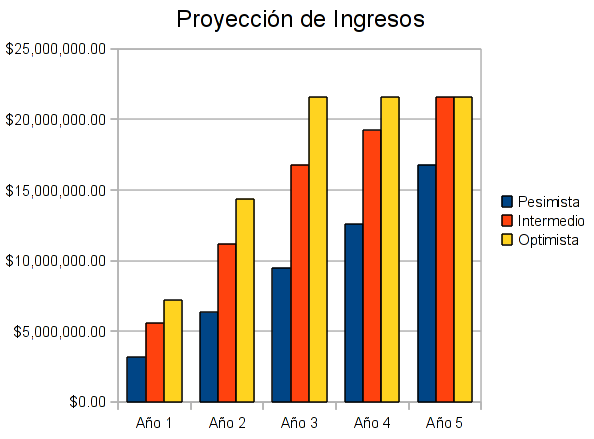
\includegraphics[scale=0.7]{images/proyeccion_ingresos}
	\caption{Proyecci\'on del Ingreso para los Primeros Cinco Años\newline (Ingreso Anual). Fuente: Elaboración Propia, 2010.}
	\label{fig:ProyeccionIngresos}
\end{figure}

\subsection{Inversión Inicial}
\label{sub:oper:InversionInicial}

La inversión inicial está compuesta por el activo fijo y el activo circulante necesario para operar; el activo circulante inicial contiene el costo de inicio de proyecto (\$951,675.00)\footnote{Ver la subsección \ref{sub:Proy:Costo}, página \pageref{sub:Proy:Costo}.

Los costos del proyecto se dividen en dos: los montos para remodelación y material inicial se incluyen en la inversión en activo fijo y los sueldos y honorarios del proyecto en el activo circulante inicial.} y una cantidad inicial de becas que se considera en \$1,000,000.00.

Se espera obtener un patrocinio inicial de \$3,000.000.00 y un crédito bancario por \$2,308,390.00. Además, se tiene intención de renovar la infraestructura (activo fijo) a lo largo del tiempo. En total, la inversión inicial es de \$ 11,579,099.40 (ver cuadro \ref{tbl:InversionInicial})

\begin{table}[h]
    \caption{Inversión Inicial}
    \label{tbl:InversionInicial}
    \centering
    \footnotesize
    \begin{tabular}{l*{6}{|r}}
	    &	\multicolumn{5}{c}{Inversiones}	& \\
	\cline{2-7}
	\multicolumn{1}{c|}{CONCEPTO}	&	\multicolumn{1}{c|}{AÑO 1}	&	\multicolumn{1}{c|}{AÑO 2}	&	\multicolumn{1}{c|}{AÑO 3}	&	\multicolumn{1}{c|}{AÑO 4}	&	\multicolumn{1}{c|}{AÑO 5}	&	\multicolumn{1}{c}{TOTAL} \\
	\hline
	\hline
	Activo Circulante	&	2,903,350.00	&	0.00	&	0.00	&	0.00	&	0.00	&	2,903,350.00 \\
	Activos Fijos	&	7,792,599.40	&	100,000.00	&	303,150.00	&	480,000.00	&	0.00	&	8,675,749.40 \\
	Activos diferidos$^{/a}$	&	0.00	&	0.00	&	0.00	&	0.00	&	0.00	&	0.00 \\
	\hline
	TOTAL	&	10,695,949.40	&	100,000.00	&	303,150.00	&	480,000.00	&	0.00	&	11,579,099.40 \\
	\hline
	\multicolumn{7}{l}{\footnotesize Fuente: Elaboración Propia, 2010.} \\
	\multicolumn{7}{l}{$^{/a}$ Ver la subsección \ref{sub:Otros:Presupuestos} para más detalles.}
    \end{tabular}
\end{table}


\subsubsection{Activo fijo}

El activo fijo está conformado por el terreno, los edificios, el mobiliario existente y las nuevas inversiiones: mobilidario nuevo, equipos de cómputo, pupitres y maquinaria de taller.

Cabe resaltar que la maquinaria de taller se estimó sobre un presupuesto base de \$500,000.00 teniendo en cuenta la pendiente elección de las carreras técnicas a impartir. Una vez definidas éstas, se actualizará el cálculo de este rubro. Los dos años siguientes se estimó un 20\% de inversión por concepto de expansión.

El cuadro \ref{tbl:ActivoFijo} muestra el presupuesto anual para activo fijo.

\begin{table}
    \caption{Presupuesto de Activos Fijos}
    \label{tbl:ActivoFijo}
    \centering
    \scriptsize
    \begin{tabular}{l|r*{5}{|@{\hspace{1mm}}c@{\hspace{1mm}}|@{\hspace{1mm}}r@{\hspace{1mm}}}}
	  & \multicolumn{1}{c|}{PRECIO} &
	    \multicolumn{2}{c|}{AÑO 1} &
	    \multicolumn{2}{c|}{AÑO 2} &
	    \multicolumn{2}{c|}{AÑO 3} &
	    \multicolumn{2}{c|}{AÑO 4} &
	    \multicolumn{2}{c}{AÑO 5} \\
	\cline{3-12}
	\multicolumn{1}{c|}{ELEMENTO} &
	    \multicolumn{1}{c|}{UNITARIO} &
	    \multicolumn{1}{c|}{C$^{/a}$} &
	    \multicolumn{1}{c|}{COSTO} &
	    \multicolumn{1}{c|}{C} &
	    \multicolumn{1}{c|}{COSTO} &
	    \multicolumn{1}{c|}{C} &
	    \multicolumn{1}{c|}{COSTO} &
	    \multicolumn{1}{c|}{C} &
	    \multicolumn{1}{c|}{COSTO} &
	    \multicolumn{1}{c|}{C} &
	    \multicolumn{1}{c}{COSTO} \\
	\hline
	\hline
	Terreno	&	3,441,776.45	&	1	&	3,441,776.45	&	0.0	&	0.00	&	0.0	&	0.00	&	0.0	&	0.00	&	0.0	&	0.00 \\
	Edificios	&	2,422,632.95	&	1	&	2,422,632.95	&	0.0	&	0.00	&	0.0	&	0.00	&	0.0	&	0.00	&	0.0	&	0.00 \\
	Mobiliario	&	346,300.00	&	0.3	&	103,890.00	&	0.0	&	0.00	&	0.0	&	0.00	&	0.0	&	0.00	&	0.0	&	0.00 \\
	Existente & & & & & & & & & & & \\
	Mobiliario Nuevo$^{/b}$	&	346,300.00	&	1	&	346,300.00	&	0.0	&	0.00	&	0.5	&	173,150.00	&	0.0	&	0.00	&	0.0	&	0.00 \\
	Computadoras	&	6,000.00	&	100	&	600,000.00	&	0.0	&	0.00	&	0.0	&	0.00	&	100.0	&	600,000.00	&	0.0	&	0.00 \\
	Pupitres	&	600.00	&	600	&	360,000.00	&	0.0	&	0.00	&	0.0	&	0.00	&	600.0	&	360,000.00	&	0.0	&	0.00 \\
	Maquinaria	&	500,000.00	&	1	&	500,000.00	&	0.2	&	100,000.00	&	0.2	&	100,000.00	&	0.0	&	0.00	&	0.0	&	0.00 \\
	de Taller & & & & & & & & & & & \\
	\hline
	TOTAL	&		&		&	7,774,599.40	&		&	100,000.00	&		&	273,150.00	&		&	960,000.00	&		&	0.00 \\
	\hline
	\multicolumn{12}{l}{\footnotesize Fuente: Elaboración Propia, 2010.} \\
	\multicolumn{12}{l}{$^{/a}$ Cantidad} \\
	\multicolumn{12}{l}{$^{/b}$ Se considera el monto inicial de insumos menos pupitres y computadoras (cuadro \ref{tbl:Proy:Insumos}, página \pageref{tbl:Proy:Insumos})} \\
    \end{tabular}
\end{table}


\subsection{Presupuesto de Egresos}

El presupuesto de egresos está compuesto por los costos\footnote{Sección \ref{sec:Costos}, página \pageref{sec:Costos}}, la depreciación y los gastos relacionados con el préstamo financiero\footnote{Sección \ref{sec:Financiamiento}, página \pageref{sec:Financiamiento}}.

\subsubsection{Depreciación}

La depreciación es la pérdida de valor de un bien. Cada año pierde un porcentaje del valor inicial hasta perder completamente su valor. Los terrenos no se deprecian, los edificios tienen una depreciación de 5\% anual y el mobiliario de 20\%; el equipo de cómputo se debe renovar cada 4 años, mientras que los pupitres cada 3; esto principalmente por el uso rudo a que están expuestos. Para la maquinaria de taller se consideró una depreciación anual de 20\%.

El cuadro \ref{tbl:Depreciacion} presenta los detalles de la depreciación.

\begin{table}
    \caption{Depreciación}
    \label{tbl:Depreciacion}
    \centering
    \scriptsize
    \begin{tabular}{@{\hspace{1mm}}l@{\hspace{1mm}}|@{\hspace{1mm}}c@{\hspace{1mm}}|@{\hspace{1mm}}r@{\hspace{1mm}}|@{\hspace{1mm}}c@{\hspace{1mm}}*{6}{|r@{\hspace{1mm}}}}
		&		&		&	DEPRECIA-	&		&		&		&		& 	\\
	ELEMENTO	&	AÑO	&	INVERSIÓN	&	CIÓN (\%)	&	\multicolumn{1}{c|}{AÑO 1}	&	\multicolumn{1}{c|}{AÑO 2}	&	\multicolumn{1}{c|}{AÑO 3}	&	\multicolumn{1}{c|}{AÑO 4}	&	\multicolumn{1}{c|}{AÑO 5}	&	\multicolumn{1}{c}{TOTAL} \\
	\hline
	\hline
	Edificios	&	1	&	2,422,632.95	&	5.00	&	121,131.65	&	121,131.65	&	121,131.65	&	121,131.65	&	121,131.65	&	605,658.24 \\
	Mobiliario	&	1	&	103,890.00	&	10.00	&	34,630.00	&	34,630.00	&	10,389.00	&	10,389.00	&	10,389.00	&	100,427.00 \\
	Existente &&&&&&&& \\
	Mobiliario	&	1	&	346,300.00	&	10.00	&	34,630.00	&	34,630.00	&	34,630.00	&	34,630.00	&	34,630.00	&	173,150.00 \\
	Nuevo		&	3	&	346,300.00	&	10.00	&	0.00	&	0.00	&	34,630.00	&	34,630.00	&	34,630.00	&	103,890.00 \\
	Computadoras	&	1	&	600,000.00	&	25.00	&	150,000.00	&	150,000.00	&	150,000.00	&	150,000.00	&	0.00	&	600,000.00 \\
			&	4	&	600,000.00	&	25.00	&	0.00	&	0.00	&	0.00	&	150,000.00	&	150,000.00	&	300,000.00 \\
	Pupitres	&	1	&	360,000.00	&	33.34	&	120,024.00	&	120,024.00	&	120,024.00	&	0.00	&	0.00	&	360,072.00 \\
			&	4	&	600.00	&	33.34	&	0.00	&	0.00	&	0.00	&	200.04	&	200.04	&	400.08 \\
	Maquinaria	&	1	&	500,000.00	&	20.00	&	100,000.00	&	100,000.00	&	100,000.00	&	100,000.00	&	100,000.00	&	500,000.00 \\
	de Taller		&	2	&	100,000.00	&	20.00	&	0.00	&	20,000.00	&	20,000.00	&	20,000.00	&	20,000.00	&	80,000.00 \\
			&	3	&	100,000.00	&	20.00	&	0.00	&	0.00	&	20,000.00	&	20,000.00	&	20,000.00	&	60,000.00 \\
	\hline
	\multicolumn{4}{r|}{TOTAL}	&	560,415.65	&	580,415.65	&	610,804.65	&	640,980.69	&	490,980.69	&	2,883,597.32 \\
	\hline
	\multicolumn{9}{l}{\footnotesize Fuente: Elaboración Propia, 2010.}
    \end{tabular}
\end{table}


\subsection{Otros Presupuestos}
\label{sub:Otros:Presupuestos}

El activo diferido está constituido por gastos pagados por anticipado, sobre los cuales se tiene el derecho de recibir un servicio aprovechable, tanto en el mismo ejercicio como en posteriores. La amortización es la aplicación a gasto de un activo diferido en proporción a su valor y al tiempo estimado de vida; la amortización anual se calcula dividendo su valor original entre el número de ejercicios que se le estima de vida probable, siempre y cuando se considere que al concluir su vida probable no tenga ningún valor\footnote{\texttt{http://www.angelfire.com/cantina/contaii/Activo\%20Diferido.htm}}.

Entre las cuentas comúnmente consideradas en el activo diferido, destacan las licencias de marca, los permisos y licencias de funcionamiento, patentes, certificaciones y cursos de capacitación.

Este proyecto no considera activos diferidos durante los primeros cinco años por las siguientes razones\footnote{Entrevista telefónica con el Pbro. Edmundo Morales Romero, S.D.B.; 24 de noviembre de 2010}:

\begin{itemize}
	\item La <<patente>> salesiana (logo, nombre, etc.) no tiene costo alguno de uso para miembros de la comunidad.
	\item No se incurre en costos por licencias y permisos de funcionamiento: información aportada por el Pbro. Edmundo Morales Romero, S.D.B., con experiencia de tres bachilleratos fundados.
	\item No se tiene contemplado de inicio adquirir certificados o cursos de certificación cuya validez haya que renovar cada cierto tiempo.
	\item El gasto publicitario está incluido en el rubro de costos fijos y se va ejerciendo sobre una base mensual.
\end{itemize}

\section{Estados Financieros Proforma}

Los estados financieros proforma son aquellos que se proyectan a futuro. Los más relevantes son el estado de resultados y el balance general.

\subsection{Estado de Resultados Proforma}

El estado de resultados proforma es aquel en donde se puede evaluar la utilidad de la empresa en un periodo de tiempo. Es por naturaleza dinámico, supone el comportamiento del dinero en un periodo de tiempo determinado. En él se integran los presupuestos relacionados con los ingresos y los costos así como los gastos financieros y los impuestos. Las observaciones e interpretación de este estado financiero se plasmarán en la sección \ref{sec:AnalisisVertical} de la página \pageref{sec:AnalisisVertical} y la sección \ref{sec:AnalisisHorizontal} de la página \pageref{sec:AnalisisHorizontal}.

El estado de resultados proforma se muestra en el cuadro \ref{tbl:EstadoResultados}.

\subsection{Balance General Proforma}

El balance general o estado de situación patrimonial indica en un momento dado cómo se encuentran los recursos de una empresa. Todo lo que posee una empresa (activo) proviene de dos fuentes: préstamos (pasivo) y aportaciones de los socios (capital).

De aquí la fórmula básica del balance general:

$$ A = P + C $$

Los comentarios e interpretación del balance general, son materia del siguiente capítulo, de momento únicamente se presenta este estado financiero en el cuadro \ref{tbl:Balance:General}.

\begin{table}
    \caption{Estado de Resultados Proyectado}
    \label{tbl:EstadoResultados}
    \centering
    \scriptsize
    \begin{tabular}{@{\hspace{1mm}}r@{\hspace{1mm}}|@{\hspace{1mm}}l@{\hspace{1mm}}*{5}{|@{\hspace{1mm}}r@{\hspace{1mm}}}}
		&	\multicolumn{1}{c|}{} 	&	\multicolumn{5}{c}{AÑO}	 \\
	\cline{3-7}
		&	\multicolumn{1}{c|}{CONCEPTO}	&	\multicolumn{1}{c|}{1}	&	\multicolumn{1}{c|}{2}	&	\multicolumn{1}{c|}{3}	&	\multicolumn{1}{c|}{4}	&	\multicolumn{1}{c}{5} \\
	\hline
	\hline
	1	&	INGRESOS NETOS	&	 5,602,800.00 	&	 11,205,600.00 	&	 16,808,400.00 	&	 19,224,000.00 	&	 21,600,000.00  \\
	\hline
	\hline
	2	&	COSTOS VARIABLES	&		&		&		&		&	 \\
	\hline
	3	&	Papelería 	&	 12,372.00 	&	 23,373.00 	&	 35,840.07 	&	 48,990.69 	&	 57,323.27  \\
	4	&	Material Didáctico	&	 13,440.00 	&	 26,460.00 	&	 42,600.60 	&	 58,344.30 	&	 69,429.72  \\
	5	&	Material talleres	&	 35,000.00 	&	 73,500.00 	&	 99,225.00 	&	 138,915.00 	&	 182,325.94  \\
	\hline
	6	&	TOTAL COSTOS VARIABLES	&	 60,812.00 	&	 123,333.00 	&	 177,665.67 	&	 246,249.99 	&	 309,078.93  \\
	\hline
	\hline
	7	&	UTILIDAD BRUTA	&	 5,541,988.00 	&	 11,082,267.00 	&	 16,630,734.33 	&	 18,977,750.01 	&	 21,290,921.07  \\
	\hline
	\hline
	8	&	COSTOS FIJOS	&		&		&		&		&	 \\
	\hline
	9	&	Servicios subcontratados	&	 836,000.00 	&	 1,570,800.00 	&	 1,649,340.00 	&	 1,731,807.00 	&	 1,818,397.35  \\
	10	&	Servicios (agua, luz, teléfono)	&	 520,000.00 	&	 546,000.00 	&	 573,300.00 	&	 601,965.00 	&	 632,063.25  \\
	11	&	Sueldos Directos	&	 2,070,750.24 	&	 3,760,368.30 	&	 5,915,755.70 	&	 7,784,415.02 	&	 8,986,902.29  \\
	\hline
	12	&	TOTAL COSTOS FIJOS	&	 3,426,750.24 	&	 5,877,168.30 	&	 8,138,395.70 	&	 10,118,187.02 	&	 11,437,362.89  \\
	\hline
	\hline
	13	&	MARGEN DE UTILIDAD	&	 2,115,237.76 	&	 5,205,098.70 	&	 8,492,338.63 	&	 8,859,562.99 	&	 9,853,558.19  \\
	\hline
	\hline
	14	&	GASTOS DE OPERACIÓN 	&		&		&		&		&	 \\
	\hline
	15	&	GASTOS DE ADMINISTRACIÓN	&		&		&		&		&	 \\
	\hline
	16	&	Sueldos Indirectos	&	 1,195,708.80 	&	 1,225,601.52 	&	 2,284,075.56 	&	 2,341,177.45 	&	 2,399,706.89  \\
	17	&	Sueldos Administrativos	&	 1,236,471.60 	&	 1,511,110.97 	&	 2,569,585.01 	&	 2,633,824.63 	&	 2,699,670.25  \\
	18	&	Depreciación anual	&	 560,415.65 	&	 580,415.65 	&	 610,804.65 	&	 640,980.69 	&	 490,980.69  \\
	\hline
	19	&	GASTOS DE VENTA	&		&		&		&		&	 \\
	\hline
	20	&	Publicidad	&	 180,000.00 	&	 189,000.00 	&	 198,450.00 	&	 208,372.50 	&	 218,791.13  \\
	\hline
	21	&	TOTAL DE GASTOS DE OPERACIÓN	&	 3,172,596.05 	&	 3,506,128.13 	&	 5,662,915.21 	&	 5,824,355.27 	&	 5,809,148.94  \\
	\hline
	22	&	GASTOS Y PRODUCTOS FINANCIEROS	&		&		&		&		&	 \\
	\hline
	23	&	Gastos Financieros 	&	 312,644.30 	&	 257,491.49 	&	 195,343.92 	&	 125,314.48 	&	 46,403.55  \\
	\hline
	24	&	TOTAL GASTOS FINANCIEROS	&	 312,644.30 	&	 257,491.49 	&	 195,343.92 	&	 125,314.48 	&	 46,403.55  \\
	\hline
	\hline
	25	&	UTILIDAD DE OPERACIÓN	&	-1,370,002.59 	&	 1,441,479.08 	&	 2,634,079.50 	&	 2,909,893.25 	&	 3,998,005.69  \\
	\hline
	\hline
	26	&	OTROS GASTOS Y PRODUCTOS	&		&		&		&		&	 \\
	\hline
	27	&	Amortización del Activo Diferido	&	 0.00 	&	 0.00 	&	 0.00 	&	 0.00 	&	 0.00  \\
	\hline
	\hline
	28	&	UTILIDAD ANTES DE IMPUESTOS	&	-1,370,002.59 	&	 1,441,479.08 	&	 2,634,079.50 	&	 2,909,893.25 	&	 3,998,005.69  \\
	\hline
	\hline
	29	&	Provisión de ISR$^{/a}$	&	 0.00 	&	 403,614.14 	&	 737,542.26 	&	 814,770.11 	&	 1,119,441.59  \\
	30	&	Provisión de PTU$^{/b}$	&	 0.00 	&	 144,147.91 	&	 263,407.95 	&	 290,989.32 	&	 399,800.57  \\
	31	&	Impuesto al Depósito en Efectivo$^{/c}$	&	 112,056.00 	&	 224,112.00 	&	 336,168.00 	&	 384,480.00 	&	 432,000.00  \\
	\hline
	32	&	TOTAL IMPUESTOS Y PRESTACIONES	&	 112,056.00 	&	 771,874.05 	&	 1,337,118.21 	&	 1,490,239.43 	&	 1,951,242.16  \\
	\hline
	\hline
	33	&	UTILIDAD DEL EJERCICIO 	&	-1,482,058.59 	&	 669,605.03 	&	 1,296,961.29 	&	 1,419,653.81 	&	 2,046,763.53  \\
	\hline
	\multicolumn{7}{l}{\footnotesize Fuente: Elaboración Propia, 2010.} \\
	\multicolumn{7}{l}{$^{/a}$ 28\% sobre utilidades antes de impuestos.} \\
	\multicolumn{7}{l}{$^{/b}$ 10\% sobre utilidades antes de impuestos.} \\
	\multicolumn{7}{l}{$^{/c}$ 2\% sobre ingresos.} \\
    \end{tabular}
\end{table}


\begin{table}
    \caption{Balance General Proforma}
    \label{tbl:Balance:General}
    \centering
    \scriptsize
    \begin{tabular}{@{\hspace{1mm}}l@{\hspace{1mm}}*{6}{|@{\hspace{1mm}}r@{\hspace{1mm}}}}
%--------------------------------------------------
    \multicolumn{1}{c|}{} &
	\multicolumn{6}{c}{AÑO}	\\
    \cline{2-7}
    \multicolumn{1}{c|}{CONCEPTO} &
	\multicolumn{1}{c|}{0} &
	\multicolumn{1}{c|}{1} &
	\multicolumn{1}{c|}{2} &
	\multicolumn{1}{c|}{3} &
	\multicolumn{1}{c|}{4} &
	\multicolumn{1}{c}{5} \\
%--------------------------------------------------
    \hline
    \hline
    ACTIVO CIRCULANTE \\
    \hline
    Caja y bancos                    &	 6,042,800.00 	&	 2,319,568.17 	&	 2,399,147.14 	&	 2,870,784.80 	&	 2,708,235.54 	&	 4,053,885.08  \\
    Cuentas por cobrar               &	 0.0 	&	 560,415.65 	&	 1,140,831.30 	&	 1,751,635.94 	&	 2,392,616.63 	&	 2,883,597.32  \\
    \hline
    TOTAL ACTIVO CIRCULANTE          &	 6,042,800.00 	&	 2,879,983.81 	&	 3,539,978.43 	&	 4,622,420.74 	&	 5,100,852.17 	&	 6,937,482.39  \\
    \hline
    ACTIVO FIJO                      &		&		&		&		&		&	 \\
    \hline
    Terreno                          &	 3,441,776.45 	&	 3,441,776.45 	&	 3,441,776.45 	&	 3,441,776.45 	&	 3,441,776.45 	&	 3,441,776.45  \\
    Edificios                        &	 2,422,632.95 	&	 2,422,632.95 	&	 2,422,632.95 	&	 2,422,632.95 	&	 2,422,632.95 	&	 2,422,632.95  \\
    Mobiliario Existente             &	 103,890.00 	&	 103,890.00 	&	 103,890.00 	&	 103,890.00 	&	 103,890.00 	&	 103,890.00  \\
    Mobiliario Nuevo                 &		&	 346,300.00 	&	 346,300.00 	&	 519,450.00 	&	 519,450.00 	&	 519,450.00  \\
    Computadoras                     &		&	 600,000.00 	&	 600,000.00 	&	 600,000.00 	&	 1,200,000.00 	&	 1,200,000.00  \\
    Pupitres                         &		&	 360,000.00 	&	 360,000.00 	&	 360,000.00 	&	 720,000.00 	&	 720,000.00  \\
    Maquinaria de Taller             &		&	 500,000.00 	&	 600,000.00 	&	 700,000.00 	&	 700,000.00 	&	 700,000.00  \\
    \hline
    DEPRECIACIÓN ACUMULADA           &		&		&		&		&		&	 \\
    \hline
    Edificios                        &	 0.0 	&	 121,131.65 	&	 242,263.30 	&	 363,394.94 	&	 484,526.59 	&	 605,658.24  \\
    Mobiliario Existente             &	 0.0 	&	 34,630.00 	&	 69,260.00 	&	 79,649.00 	&	 90,038.00 	&	 100,427.00  \\
    Mobiliario Nuevo año 1           &	 0.0 	&	 34,630.00 	&	 69,260.00 	&	 103,890.00 	&	 138,520.00 	&	 173,150.00  \\
    Mobiliario nuevo año 3           &	 0.0 	&	 0.0 	&	 0.0 	&	 34,630.00 	&	 69,260.00 	&	 103,890.00  \\
    Computadoras año 1               &	 0.0 	&	 150,000.00 	&	 300,000.00 	&	 450,000.00 	&	 600,000.00 	&	 600,000.00  \\
    Computadoras año 4               &	 0.0 	&	 0.0 	&	 0.0 	&	 0.0 	&	 150,000.00 	&	 300,000.00  \\
    Pupitres año 1                   &	 0.0 	&	 120,024.00 	&	 240,048.00 	&	 360,072.00 	&	 360,072.00 	&	 360,072.00  \\
    Pupitres año 4                   &	 0.0 	&	 0.0 	&	 0.0 	&	 0.0 	&	 200.04 	&	 400.08  \\
    Maquinaria de Taller año 1       &	 0.0 	&	 100,000.00 	&	 200,000.00 	&	 300,000.00 	&	 400,000.00 	&	 500,000.00  \\
    Maquinaria de Taller año 2       &	 0.0 	&	 0.0 	&	 20,000.00 	&	 40,000.00 	&	 60,000.00 	&	 80,000.00  \\
    Maquinaria de Taller año 3       &	 0.0 	&	 0.0 	&	 0.0 	&	 20,000.00 	&	 40,000.00 	&	 60,000.00  \\
    \hline
    TOTAL ACTIVO FIJO                &	 5,968,299.40 	&	 7,214,183.75 	&	 6,733,768.11 	&	 6,396,113.46 	&	 6,715,132.77 	&	 6,224,152.08  \\
    \hline
    ACTIVO DIFERIDO                  &		&		&		&		&		&	 \\
    \hline
    Licencias y Permisos             &	 0.0 	&	 0.0 	&	 0.0 	&	 0.0 	&	 0.0 	&	 0.0  \\
    \hline
    TOTAL ACTIVO DIFERIDO            &	 0.0 	&	 0.0 	&	 0.0 	&	 0.0 	&	 0.0 	&	 0.0  \\
    \hline
    \hline
    TOTAL ACTIVO                     &	 12,011,099.40 	&	 10,094,167.57 	&	 10,273,746.54 	&	 11,018,534.20 	&	 11,815,984.94 	&	 13,161,634.48  \\
    \hline
    \hline
    PASIVO                           &		&		&		&		&		&	 \\
    \hline
    Crédito                          &	 2,800,390.00 	&	 2,365,516.75 	&	 1,875,490.69 	&	 1,323,317.06 	&	 701,113.99 	&	 0.00  \\
    \hline
    TOTAL DE PASIVO                  &	 2,800,390.00 	&	 2,365,516.75 	&	 1,875,490.69 	&	 1,323,317.06 	&	 701,113.99 	&	 0.00  \\
    \hline
    CAPITAL SOCIAL                   &	 9,210,709.40 	&	 9,210,709.40 	&	 9,210,709.40 	&	 9,210,709.40 	&	 9,210,709.40 	&	 9,210,709.40  \\
    \hline
    Utilidad del Ejercicio           &	 0.0 	&	-1,482,058.59 	&	 669,605.03 	&	 1,296,961.29 	&	 1,419,653.81 	&	 2,046,763.53  \\
    Utilidad del Ejercicio Acumulada &	 0.0 	&	 0.0 	&	-1,482,058.59 	&	-812,453.55 	&	 484,507.74 	&	 1,904,161.55  \\
    \hline
    TOTAL CAPITAL CONTABLE           &	 9,210,709.40 	&	 7,728,650.81 	&	 8,398,255.85 	&	 9,695,217.14 	&	 11,114,870.95 	&	 13,161,634.48  \\
    \hline
    \hline
    TOTAL PASIVO MAS CAPITAL         &	 12,011,099.40 	&	 10,094,167.57 	&	 10,273,746.54 	&	 11,018,534.20 	&	 11,815,984.94 	&	 13,161,634.48  \\
    \hline
%--------------------------------------------------
	\multicolumn{7}{l}{\footnotesize Fuente: Elaboración Propia, 2010.}
    \end{tabular}
\end{table}




\chapter{Administración de Finanzas}
\label{cap:Admin:Finanzas}

En el presente capítulo se analizan diversos aspectos relacionados con la estructura financiera del proyecto. El \emph{Punto de Equilibro} es uno de los indicadores de éxito del proyecto, el cual se complementa con las \emph{Utilidades}. Otro de los criterios para determinar la viabilidad financiera del proyecto es el saldo positivo en el \emph{Flujo de Efectivo} al menos al finalizar el periodo de evaluación de cinco años.

Posteriormente se examina la estructura de los \emph{Activos y Pasivos} y las características principales del \emph{Financiamiento Requerido}. La comunidad salesiana posee ya un inmueble, en la sección \emph{Contribución de Capital} se resaltan algunos aspectos relevantes sobre el mismo desde el punto de vista financiero-contable.

Por último se hace mención a la posibilidad de obtención de \emph{Recursos Colaterales}; estos recursos no son considerados en la contabilidad sino que se muestran con fines descriptivos.\footnote{Los motivos de este enfoque se encuentran en la \nameref{ch:Introduccion} a partir de la página \pageref{ch:Introduccion}.}

\section{Punto de Equilibrio}

Mediante el cálculo del punto de equilibrio se pretende determinar el alumnado mínimo necesario para que la institución no incurra en pérdidas\footnote{Consúltense las siguientes fuentes para esta sección: \citep{Van2003fundamentos, novoa2008finanzas, bodie2003finanzas}}.

El punto de equilibrio se obtiene algebráicamente de la siguiente forma:

$$
	\begin{array}{rcl}
		P \cdot U &=& C_{vu} \cdot U + C_f \\
		\left( P - C_{vu} \right) \cdot U &=& C_f \\
		U &=& \frac{C_f}{P - C_{vu}}
	\end{array}
$$

Donde:

\begin{description}
	\item[$P$] Precio de venta unitario
	\item[$U$] Unidades del punto de equilibrio
	\item[$C_{vu}$] Costo variable unitario
	\item[$C_f$] Costo fijo
\end{description}

El cuadro \ref{tbl:PuntoEquilibrio} muestra el punto de equilibrio, a excepción del primer año, el resto del periodo estudiado se rebasa este punto de equilibrio; lo cual puede corroborarse con las utilidades en el estado de resultados.

\begin{table}
    \caption{Punto de Equilibrio}
    \label{tbl:PuntoEquilibrio}
    \centering
    \footnotesize
    \begin{tabular}{@{\hspace{1mm}}l@{\hspace{1mm}}*{5}{|@{\hspace{1mm}}r@{\hspace{1mm}}}}
	%-------------------------------------------------- \\
	\hline
	\multicolumn{1}{c|}{CONCEPTO} &
	    \multicolumn{1}{c|}{AÑO 1} &
	    \multicolumn{1}{c|}{AÑO 2} &
	    \multicolumn{1}{c|}{AÑO 3} &
	    \multicolumn{1}{c|}{AÑO 4} &
	    \multicolumn{1}{c}{AÑO 5} \\
	\hline
	\hline
	%-------------------------------------------------- \\
	Ingreso por Unidad	&	2,100.00	&	2,100.00	&	2,100.00	&	1,800.00	&	1,800.00 \\
	Mensual &&&&& \\
	Costos Variables	&	22.72	&	23.10	&	22.20	&	23.06	&	25.76 \\
	por Unidad Mensual &&&&& \\
	Margen de Contribución	&	2,077.28	&	2,076.90	&	2,077.80	&	1,776.94	&	1,774.24 \\
	por Unidad Mensual &&&&& \\
	%-------------------------------------------------- \\
	\hline
	Costos Fijos Anuales	&	6,038,930.64	&	8,802,880.79	&	13,190,506.27	&	15,301,561.60	&	16,755,531.14 \\
	Margen de Contribución	&	24,927.30	&	24,922.85	&	24,933.63	&	21,323.31	&	21,290.92 \\
	por Unidad Anual &&&&& \\
	\hline
	\hline
	PUNTO DE EQUILIBRIO	&	242	&	353	&	529	&	718	&	787 \\
	%-------------------------------------------------- \\
	\hline
	\multicolumn{6}{l}{\footnotesize Fuente: Elaboración Propia, 2010.}
    \end{tabular}
\end{table}


\section{Utilidades}

Con la finalidad de comparar mejor el punto de equilibrio, se presenta a continuación la parte que se refiere a las utilidades juntamente con la matrícula esperada para cada año (cuadro \ref{tbl:Utilidades}).

El ejercicio del primer año otorga pérdidas, sin embargo, el resto de los años traen utilidades y lo realizan en forma creciente. Esto a pesar de que el precio de la colegiatura no se incrementa con la inflación y el porcentaje de becas se incrementa al incrementar la matrícula estudiantil.

\begin{table}[h]
    \caption{Utilidades}
    \label{tbl:Utilidades}
    \centering
    \footnotesize
    \begin{tabular}{l*{5}{|r}}
	\multicolumn{1}{c|}{CONCEPTO} &
	    \multicolumn{1}{c|}{1} &
	    \multicolumn{1}{c|}{2} &
	    \multicolumn{1}{c|}{3} &
	    \multicolumn{1}{c|}{4} &
	    \multicolumn{1}{c}{5} \\
	\hline
	\hline
	Utilidad del Ejercicio	&	-1,482,058.59 	&	 669,605.03 	&	 1,296,961.29 	&	 1,419,653.81 	&	 2,046,763.53 \\
	Matrícula	&	222	&	445	&	667	&	290	&	1000 \\
	\hline
	\multicolumn{6}{l}{\footnotesize Fuente: Elaboración Propia, 2010.}
    \end{tabular}
\end{table}



\clearpage
\section{Flujo de Efectivo}

A continuación se presentan dos instrumentos financieros con amplia relación: el estado de origen y aplicación de los recursos y el flujo neto de efectivo.

\subsection{Origen y Aplicación de los Recursos}

El estado de origen y aplicación de los recursos describe la forma en que una empresa obtiene y utiliza los fondos monetarios, nos permite evaluar si el proyecto tendrá el efectivo necesario para hacer frente a sus obligaciones, entendidas éstas como cubrir los costos y pagar las deudas. El cuadro \ref{tbl:OrigenAplicacion} muestra cómo este proyecto tiene la liquidez necesaria, lo cual se puede ver en el último renglón donde todas las cifras son positivas.

En términos de liquidez, puede observarse que los primeros dos años y el cuarto son los más difíciles. De los primeros dos, la causa se debe a que en el primer año se tienen pérdidas por no haber alcanzado el punto de equilibrio, del cuarto año, la razón es que por una parte se incrementó el organigrama y por otro lado disminuyen los ingresos por estudiante debido a un mayor porcentaje de becas otorgado como consecuencia de tener una matrícula estudiantil mayor.

Por último, aclarar que la cuenta de saldo en caja y bancos\footnote{Parte del activo circulante} proviene de este instrumento; y es precisamente el rubro de \emph{saldo final de efectivo}.

\begin{table}[h]
    \caption{Estado de Origen y Aplicación de Recursos}
    \label{tbl:OrigenAplicacion}
    \centering
    \scriptsize
    \begin{tabular}{@{\hspace{1mm}}r@{\hspace{1mm}}l@{\hspace{1mm}}*{6}{|@{\hspace{1mm}}r@{\hspace{1mm}}}}
	& \multicolumn{1}{c|}{CONCEPTO} &
	    \multicolumn{1}{c|}{AÑO 0} &
	    \multicolumn{1}{c|}{AÑO 1} &
	    \multicolumn{1}{c|}{AÑO 2} &
	    \multicolumn{1}{c|}{AÑO 3} &
	    \multicolumn{1}{c|}{AÑO 4} &
	    \multicolumn{1}{c}{AÑO 5} \\
    \hline
    \hline
      & SALDO INICIAL DE EFECTIVO             &  12,011,099.40 	&	 6,042,800.00 	&	 2,319,568.17 	&	 2,399,147.14 	&	 2,870,784.80 	&	 2,708,235.54  \\
    \hline
      & Ingresos Para el Año n+1              & 0.0 	&	 5,602,800.00 	&	 11,205,600.00 	&	 16,808,400.00 	&	 19,224,000.00 	&	 21,600,000.00  \\
    + & Entradas de efectivo                  &  0.0 	&	 5,602,800.00 	&	 11,205,600.00 	&	 16,808,400.00 	&	 19,224,000.00 	&	 21,600,000.00  \\
    \hline
    = & DISPONIBILIDAD DE EFECTIVO            &  12,011,099.40 	&	 11,645,600.00 	&	 13,525,168.17 	&	 19,207,547.14 	&	 22,094,784.80 	&	 24,308,235.54  \\
    \hline
      & Total Costos Variables                &  0.0 	&	 60,812.00 	&	 123,333.00 	&	 177,665.67 	&	 246,249.99 	&	 309,078.93  \\
      & Total Costos Fijos & 0.0 	&	 3,426,750.24 	&	 5,877,168.30 	&	 8,138,395.70 	&	 10,118,187.02 	&	 11,437,362.89  \\
      & (Sin Depreciación) &&&&& \\
      & Total de Gastos de Operación          & 0.0 	&	 3,172,596.05 	&	 3,506,128.13 	&	 5,662,915.21 	&	 5,824,355.27 	&	 5,809,148.94  \\
      & Total Gastos financieros              &  0.0 	&	 312,644.30 	&	 257,491.49 	&	 195,343.92 	&	 125,314.48 	&	 46,403.55  \\
      & Pago de ISR y PTU                     &  0.0 	&	 0.0 	&	 547,762.05 	&	 1,000,950.21 	&	 1,105,759.43 	&	 1,519,242.16  \\
      & Impuesto al Depósido en Efectivo      & 0.0 	&	 112,056.00 	&	 224,112.00 	&	 336,168.00 	&	 384,480.00 	&	 432,000.00  \\
      & Pago de crédito (Capital)             & 0.0 	&	 434,873.25 	&	 490,026.06 	&	 552,173.63 	&	 622,203.07 	&	 701,113.99  \\
      & Inversión en Terrenos                 & 3,441,776.45 	&	 0.0 	&	 0.0 	&	 0.0 	&	 0.0 	&	 0.0  \\
      & Inversión en Edificios                & 2,422,632.95 	&	 0.0 	&	 0.0 	&	 0.0 	&	 0.0 	&	 0.0  \\
      & Inversión en Mobiliario y Equipos     & 103,890.00 	&	 1,806,300.00 	&	 100,000.00 	&	 273,150.00 	&	 960,000.00 	&	 0.0  \\
    \hline
    - & SALIDAS DE EFECTIVO                   &  5,968,299.40	&	9,326,031.83	&	11,126,021.03	&	16,336,762.34	&	19,386,549.25	&	20,254,350.47 \\
    \hline
    \hline
    = & SALDO FINAL DE EFECTIVO               &  6,042,800.00	&	2,319,568.17	&	2,399,147.14	&	2,870,784.80	&	2,708,235.54	&	4,053,885.08 \\
    \hline
    \multicolumn{8}{l}{\footnotesize Fuente: Elaboración Propia, 2010.}
    \end{tabular}
\end{table}



\subsection{Flujo Neto de Efectivo}
\label{sub:FNE}

El flujo neto de efectivo (FNE) se parece al estado de origen y aplicación de los recursos en que describe cómo se obtienen y utilizan los recursos en una organización.\footnote{La siguiente explicación corresponde al flujo neto de efectivo acumulado.}

Sin embargo tiene una diferencia capital: el monto de la inversión inicial se coloca con signo negativo, lo mismo que sucesivas inversiones en caso de existir. En el contexto de evaluación de proyectos, esto permite evaluar la capacidad de la empresa para recuperar lo invertido. Al inversionista (y al accionista) le interesa saber en qué medida se recupera el capital invertido en comparación con otras ofertas. Es la materia prima de la evaluación final de un proyecto. En el capítulo \ref{cap:Evaluacion:Financiera} (página \pageref{cap:Evaluacion:Financiera}) se retomará este tema precisamente para validar la viabilidad del bachillerato.

Conviene, llegados a este punto, realizar una aclaración: aunque el monto total de la inversión inicial es de \$12,011,099.40, los \$6,210,709.40 que conforman el inmueble (terreno y edificios) y mobiliario existentes son prescindibles en este análisis; la razón es que se trata de un capital del que no hay accionistas que pedirán cuentas y al que no se le dará otro uso si no es la escuela. En ese sentido es un \emph{capital muerto}.

Esta consideración lleva a plantear dos escenarios: con inmueble y mobiliario existentes y sin ellos. Los inversionistas para este proyecto que reclamarán resultados sobre sus aportaciones son las empresas patrocinadoras.

Por esta razón, el cuadro \ref{tbl:FNE} presenta al final un resumen con los resultados más relevantes cuando se prescinde de la infraestructura con la que se cuenta actualmente. Los datos de este resumen son los utilizados en el capitulo \ref{cap:Evaluacion:Financiera} para realizar la evaluación financiera.

\begin{table}
    \caption{Flujo Neto de Efectivo}
    \label{tbl:FNE}
    \centering
    \scriptsize
    \begin{tabular}{@{\hspace{1mm}}r@{\hspace{1mm}}|@{\hspace{1mm}}l@{\hspace{1mm}}*{6}{|@{\hspace{1mm}}r@{\hspace{1mm}}}}
	%--------------------------------------------------
	& \multicolumn{1}{c|}{CONCEPTO} &
	    \multicolumn{1}{c|}{AÑO 1} &
	    \multicolumn{1}{c|}{AÑO 2} &
	    \multicolumn{1}{c|}{AÑO 3} &
	    \multicolumn{1}{c|}{AÑO 4} &
	    \multicolumn{1}{c}{AÑO 5} \\
	%--------------------------------------------------
	\hline
	\hline
	& \multicolumn{7}{c}{FLUJO NETO DE EFECTIVO CONSIDERANDO \emph{CAPITAL MUERTO}} \\
	\hline
	\hline
	1	&	Inversion Inicial                & -12,011,099.40 & & & & & \\
	\hline
	2	&	SALDO INICIAL                    &                & -12,011,099.40 	&	-12,932,742.34 	&	-11,682,721.66 	&	-9,774,955.72 	&	-7,714,321.22  \\
	\hline
	3	&	Ingresos Netos                   &                &  5,602,800.00 	&	 11,205,600.00 	&	 16,808,400.00 	&	 19,224,000.00 	&	 21,600,000.00  \\
	\hline
	4	&	TOTAL DE INGRESOS                &                & -6,408,299.40 	&	-1,727,142.34 	&	 5,125,678.34 	&	 9,449,044.28 	&	 13,885,678.78  \\
	\hline
	\hline
	5	&	\multicolumn{7}{l}{COSTOS VARIBALES} \\
	\hline
	6	&	Papelería                        &                &  12,372.00 	&	 23,373.00 	&	 35,840.07 	&	 48,990.69 	&	 57,323.27  \\
	7	&	Material Didáctico               &                &  13,440.00 	&	 26,460.00 	&	 42,600.60 	&	 58,344.30 	&	 69,429.72  \\
	8	&	Material talleres                &                &  35,000.00 	&	 73,500.00 	&	 99,225.00 	&	 138,915.00 	&	 182,325.94  \\
	\hline
	9	&	TOTAL COSTOS VARIBLES            &                &  60,812.00 	&	 123,333.00 	&	 177,665.67 	&	 246,249.99 	&	 309,078.93  \\
	\hline
	10	&	UTILIDAD BRUTA                   &                & -6,469,111.40 	&	-1,850,475.34 	&	 4,948,012.67 	&	 9,202,794.29 	&	 13,576,599.85  \\
	\hline
	\hline
	11	&	\multicolumn{7}{l}{COSTOS FIJOS} \\
	\hline
	12	&	Servicios subcontratados         &                &  836,000.00 	&	 1,570,800.00 	&	 1,649,340.00 	&	 1,731,807.00 	&	 1,818,397.35  \\
	13	&	Servicios (agua, luz, telefono)  &                &  520,000.00 	&	 546,000.00 	&	 573,300.00 	&	 601,965.00 	&	 632,063.25  \\
	14	&	Sueldos Directos                 &                &  2,070,750.24 	&	 3,760,368.30 	&	 5,915,755.70 	&	 7,784,415.02 	&	 8,986,902.29  \\
	\hline
	15	&	TOTAL COSTOS FIJOS               &                &  3,426,750.24 	&	 5,877,168.30 	&	 8,138,395.70 	&	 10,118,187.02 	&	 11,437,362.89  \\
	\hline
	16	&	MARGEN DE UTILIDAD               &                & -9,895,861.64 	&	-7,727,643.64 	&	-3,190,383.03 	&	-915,392.73 	&	 2,139,236.97  \\
	\hline
	\hline
	17	&	\multicolumn{7}{l}{GASTOS DE OPERACIÓN} \\
	\hline
	18	&	\multicolumn{7}{l}{GASTOS DE ADMINISTRACION} \\
	\hline
	19	&	Sueldos Indirectos               &                &  1,195,708.80 	&	 1,225,601.52 	&	 2,284,075.56 	&	 2,341,177.45 	&	 2,399,706.89  \\
	20	&	Sueldos Administrativos          &                &  1,236,471.60 	&	 1,511,110.97 	&	 2,569,585.01 	&	 2,633,824.63 	&	 2,699,670.25  \\
	\hline
	21	&	\multicolumn{7}{l}{GASTOS DE VENTA} \\
	\hline
	22	&	Publicidad                       &                &  180,000.00 	&	 189,000.00 	&	 198,450.00 	&	 208,372.50 	&	 218,791.13  \\
	\hline
	23	&	TOTAL DE GASTOS     &                &  2,612,180.40 	&	 2,925,712.49 	&	 5,052,110.57 	&	 5,183,374.58 	&	 5,318,168.26  \\
		&	DE OPERACIÓN & & & & & \\
	\hline
	24	&	\multicolumn{7}{l}{GASTOS Y PRODUCTOS FINANCIEROS} \\
	\hline
	25	&	Gastos Financieros               &                &  312,644.30 	&	 257,491.49 	&	 195,343.92 	&	 125,314.48 	&	 46,403.55  \\
	\hline
	26	&	TOTAL GASTOS         &                &  312,644.30 	&	 257,491.49 	&	 195,343.92 	&	 125,314.48 	&	 46,403.55  \\
		&	FINANCIEROS & & & & & \\
	\hline
	27	&	UTILIDAD DE OPERACIÓN            &                & -12,820,686.34 	&	-10,910,847.61 	&	-8,437,837.51 	&	-6,224,081.79 	&	-3,225,334.85  \\
	\hline
	\hline
	28	&	\multicolumn{7}{l}{OTROS GASTOS Y PRODUCTOS} \\
	\hline
	29	&	UTILIDAD ANTES      &                & -12,820,686.34 	&	-10,910,847.61 	&	-8,437,837.51 	&	-6,224,081.79 	&	-3,225,334.85  \\
		&	DE IMPUESTOS & & & & & \\
	\hline
	\hline
	30	&	Provision de ISR                 &                &  0.0 	&	 403,614.14 	&	 737,542.26 	&	 814,770.11 	&	 1,119,441.59  \\
	31	&	Provision de PTU                 &                &  0.0 	&	 144,147.91 	&	 263,407.95 	&	 290,989.32 	&	 399,800.57  \\
	32	&	Impuesto al Depósido &                &  112,056.00 	&	 224,112.00 	&	 336,168.00 	&	 384,480.00 	&	 432,000.00  \\
		& en Efectivo & & & & & \\
	\hline
	33	&	TOTAL IMPUESTOS                  &                &  112,056.00 	&	 771,874.05 	&	 1,337,118.21 	&	 1,490,239.43 	&	 1,951,242.16  \\
	\hline
	\hline
	34	&	FLUJOS NETOS         & -12,011,099.40 & -12,932,742.34 	&	-11,682,721.66 	&	-9,774,955.72 	&	-7,714,321.22 	&	-5,176,577.01  \\
		&	DE EFECTIVO & & & & & \\
	\hline
	\hline
	& \multicolumn{7}{c}{FLUJO NETO DE EFECTIVO SIN CONSIDERAR \emph{CAPITAL MUERTO}} \\
	%--------------------------------------------------
	\hline
	\hline
	1	&	Inversion Inicial                & -5,800,390.00 & & & & & \\
	\hline
	2	&	SALDO INICIAL                    &               & -5,800,390.00 	&	-6,722,032.94 	&	-5,472,012.26 	&	-3,564,246.32 	&	-1,503,611.82  \\
	\hline
	34	&	FLUJOS NETOS         & -5,800,390.00 & -6,722,032.94 	&	-5,472,012.26 	&	-3,564,246.32 	&	-1,503,611.82 	&	 1,034,132.39  \\
		&	DE EFECTIVO & & & & & \\
	\hline
	\multicolumn{8}{l}{\footnotesize Fuente: Elaboración Propia, 2010.}
    \end{tabular}
\end{table}


\section{Activos y Pasivos}
\label{sec:ActivosPasivos}

En esta sección se comentan algunos aspectos relevantes sobre la estructura de activos y pasivos previstos en el bachillerato.

El cuadro \ref{tbl:Activo:Resumen} presenta las cuentas del activo y el pasivo sobre las que versará la discusión.

Las principales observaciones sobre las cuentas de activo y pasivo relevantes son:

\begin{description}
	\item[Caja y Bancos] Con recuperación creciente (a excepción del año 4 debido al aumento de porcentaje de becas y la inversión en activo fijo) en el periodo de 5 años no alcanza a empatar la inversión inicial de su rubro.
	\item[Cuentas por Cobrar] Se trata de una \emph{cuenta virtual} consecuencia de la depreciación. La razón es que no se renueva el activo fijo en el mismo ritmo que se deprecia.
	\item[Activo Fijo] El activo fijo incrementa su valor en los años 1 y 4 debido a las fuertes inversiones realizadas esos años. El resto de los años disminuye el valor debido a la depreciación.
	\item[Total Activo] Después de una caída el primer año, el total del activo se incrementa y para el quinto año es mayor al activo inicial.
	\item[Pasivo: Crédito] El pago del crédito concluye en el año 5. De momento no se tiene proyectado solicitar un préstamo similar los siguientes cinco años.
\end{description}

Considerando estas observaciones, la conclusión apunta en el sentido de que este proyecto se percibe más sólido financieramente en su segundo lustro de operación: sin una carga financiera considerable y con utilidades como las del último año se perfila hacia la consolidación. Convendría realizar un estudio considerando una ventana de tiempo de 10 años que mostrara con mayor claridad su viabilidad y conveniencia financiera.

\begin{table}
    \caption{Cuentas Relevantes del Activo y el Pasivo}
    \label{tbl:Activo:Resumen}
    \centering
    \scriptsize
    \begin{tabular}{@{\hspace{1mm}}l@{\hspace{1mm}}*{6}{|@{\hspace{1mm}}r@{\hspace{1mm}}}}
%--------------------------------------------------
    \multicolumn{1}{c|}{} &
	\multicolumn{6}{c}{AÑO}	\\
    \cline{2-7}
    \multicolumn{1}{c|}{CONCEPTO} &
	\multicolumn{1}{c|}{0} &
	\multicolumn{1}{c|}{1} &
	\multicolumn{1}{c|}{2} &
	\multicolumn{1}{c|}{3} &
	\multicolumn{1}{c|}{4} &
	\multicolumn{1}{c}{5} \\
%--------------------------------------------------
    \hline
    \hline
    ACTIVO CIRCULANTE \\
    Caja y bancos                    &	 6,042,800.00 	&	 2,319,568.17 	&	 2,399,147.14 	&	 2,870,784.80 	&	 2,708,235.54 	&	 4,053,885.08  \\
    Cuentas por cobrar               &	 0.0 	&	 560,415.65 	&	 1,140,831.30 	&	 1,751,635.94 	&	 2,392,616.63 	&	 2,883,597.32  \\
    \hline
    ACTIVO FIJO                      &		&		&		&		&		&	 \\
    TOTAL ACTIVO FIJO                &	 5,968,299.40 	&	 7,214,183.75 	&	 6,733,768.11 	&	 6,396,113.46 	&	 6,715,132.77 	&	 6,224,152.08  \\
    \hline
    TOTAL ACTIVO                     &	 12,011,099.40 	&	 10,094,167.57 	&	 10,273,746.54 	&	 11,018,534.20 	&	 11,815,984.94 	&	 13,161,634.48  \\
    \hline
    PASIVO                           &		&		&		&		&		&	 \\
    \hline
    Crédito                          &	 2,800,390.00 	&	 2,365,516.75 	&	 1,875,490.69 	&	 1,323,317.06 	&	 701,113.99 	&	 0.00  \\
%--------------------------------------------------
	\hline
	\multicolumn{7}{l}{\footnotesize Fuente: Elaboración Propia, 2010.}
    \end{tabular}
\end{table}



\section{Financiamiento Requerido}
\label{sec:Financiamiento}

Para hacer realidad este proyecto se necesita un financiamiento considerado desde dos aspectos: por un lado, la solicitud de un préstamo a una tasa de interés conveniente; por otra parte, la búsqueda de patrocinios y donativos.

En esta sección se hablará sobre el préstamo y en la siguiente sobre los patrocinios y donativos.

\subsection{Características del Préstamo}

Se propone la solicitud de un financiamiento ante la Secretaría de Economía por ofrecer bajas tasas de interés en comparación con entidades privadas (cuadro \ref{tbl:Credito}).

Las condiciones del financiamiento son:

\begin{itemize}
	\item Monto del crédito: \$2,800,390.00 M.N.
	\item Interés anual: 12\%.
	\item Periodo de recuperación: 5 años.
	\item Número de pagos: 60 pagos mensuales.
	\item Pago mensual: \$62,293.13 M.N.
	\item No se ofrece periodo de gracia.
\end{itemize}

Las áreas principales de aplicación son: capital de trabajo y remodelaciones.

\begin{table}
    \caption{Tabla de Amortización Anual del Crédito}
    \label{tbl:Credito}
    \centering
    \footnotesize
    \begin{tabular}{c*{5}{|r}}
    %--------------------------------------------------
	&   \multicolumn{1}{c|}{SALDO} &
	    \multicolumn{1}{c|}{PAGO DE} &
	    \multicolumn{1}{c|}{PAGO} \\
	\multicolumn{1}{c|}{AÑO} &
	    \multicolumn{1}{c|}{INICIAL} &
	    \multicolumn{1}{c|}{INTERÉS} &
	    \multicolumn{1}{c|}{PRINCIPAL} &
	    \multicolumn{1}{c|}{PAGO TOTAL} &
	    \multicolumn{1}{c}{SALDO FINAL} \\
	\hline
	\hline
	1	&	2,800,390.00	&	312,644.30	&	434,873.25	&	747,517.55	&	2,365,516.75 \\
	2	&	2,365,516.75	&	257,491.49	&	490,026.06	&	747,517.55	&	1,875,490.69 \\
	3	&	1,875,490.69	&	195,343.92	&	552,173.63	&	747,517.55	&	1,323,317.06 \\
	4	&	1,323,317.06	&	125,314.48	&	622,203.07	&	747,517.55	&	701,113.99 \\
	5	&	701,113.99	&	46,403.55	&	701,113.99	&	747,517.55	&	0.00 \\
    %--------------------------------------------------
    \hline
    \multicolumn{6}{l}{\footnotesize Fuente: Elaboración Propia, 2010.}
    \end{tabular}
\end{table}


\section{Contribución de Capital}
\label{sec:Capital}

Como se señaló en el cuadro \ref{tbl:ActivoFijo} (página \pageref{tbl:ActivoFijo}), se cuenta con una infraestructura equivalente a \$6,210,709.40 M.N. entre terreno, edificios y mobiliario existente.

Adicionalmente, se desea obtener un patrocinio inicial equivalente a \$3,000,000.00 tanto para iniciar el proyecto como para ofrecer becas.

La posibilidad de conseguir esos patrocinios (en dinero o en especie) se basa en las experiencias exitosas de Saltillo y San Luis Potosí, donde incluso se donaron terrenos para esas escuelas (subsección \ref{sub:Patrocinios}, página \pageref{sub:Patrocinios}).

En total, el capital inicial es de \$9,210,709.40 M.N.; sin embargo, para efectos de evaluación financiera se debe considerar que las instalaciones existentes actualmente son \emph{capital muerto}, es decir, de no usarse para el bachillerato no se usarían para ninguna otra inversión\footnote{Subsección \ref{sub:FNE}, página \pageref{sub:FNE}}.

\section{Recursos Colaterales}
\label{sec:RecursosColaterales}

Adicionalmente a las colegiaturas, se pretende obtener de forma permanente donativos y patrocinios (ya sea en efectivo o en especie) que abaraten los costos e incrementen el fondo de becas.\footnote{Sin embargo, la estrategia para obtener dicho patrocinio está fuera del alcance del presente trabajo y la corrida financiera no contempla ninguna fuente alterna salvo la mencionada en la inversión inicial (ver \ref{sub:intro:Limitaciones} <<\nameref{sub:intro:Limitaciones}>> en la página \pageref{sub:intro:Limitaciones}.}

Para esto, se tienen previstas diferentes modalidades de patrocinios, entre otras:

\begin{itemize}
	\item Adopta un estudiante.
	\item Adopta un profesor.
	\item Patrocinio para equipar la escuela (equipos de cómputo y maquinaria de taller).
	\item Patrocinio para insumos de la escuela: papelería, material de talleres.
	\item Paquete especial para hijos de los trabajadores de la empresa.
	\item Apoyo a los estudiantes talentosos.
\end{itemize}

Similar a la pirámide de necesidades del mercado\footnote{Sección \ref{sec:Clientes}, página \pageref{sec:Clientes}}, se propone una pirámide de donadores de la siguiente forma:

\begin{itemize}
	\item Dos o tres patrocinadores grandes que cubran lo equivalente a 30 estudiantes cada uno.
	\item Diez a veinte patrocinadores medianos que cubran lo equivalente a 10 estudiantes cada uno.
	\item Cincuenta a cien patrocinadores pequeños que bequen a un estudiante cada uno.
	\item Apoyo general de la comunidad mediante aportaciones voluntarias en efectivo o especie.
\end{itemize}

Otras actividades para obtener recursos o ahorros adicionales son:

\begin{itemize}
	\item Profesores honorarios que donen algunas horas de su tiempo a la semana dando clase sin cobrar.
	\item Cooperativa escolar.
	\item Servicios a las empresas por parte de los estudiantes (programa de becarios).
	\item Conseguir apoyo de fundaciones (e.g. bécalos).
\end{itemize}


\chapter{Análisis Financiero}
\label{cap:AnalsisFinanciero}

En este capítulo se analiza financieramente el proyecto con el fin de identificar características que lo hagan más atractivo a posibles patrocinadores y entidades financieras que otorguen préstamos. Está dividido en tres partes, en la primera (análisis estructural o vertical) se analizará la estructura intemporal del estado de resultados, en la segunda (análisis intertemporal u horizontal) se revisará su evolución en el tiempo y en la tercera (razones financieras) se extraerán variables que describan el proyecto.

Tanto el análisis vertical como el horizontal pueden realizarse igualmente sobre el balance general, sin embargo, para entidades crediticias y patrocinadores son mucho más relevantes estos análisis sobre el estado de resultados proforma\footnote{Para el análisis vertical y el horizontal se realizó una redacción propia a partir de las siguientes fuentes: \citep{brock1987contabilidad, mejia2006diccionario, dobarganes2005contabilidad}}.

\section{Análisis estructural o vertical}
\label{sec:AnalisisVertical}

El análisis estructural o vertical identifica la estructura del estado de resultados en términos de porcentajes sobre los ingresos netos. Permite identificar qué aspecto o rubro impacta con mayor fuerza en la reducción de las utilidades, así como la relación entre utilidades e ingresos.

Observaciones sobre el análisis vertical (cuadros \ref{tbl:Vertical:1} y \ref{tbl:Vertical:2}):

\begin{itemize}
	\item La utilidad bruta se mantiene proporcionalmente casi constante con variaciones menores al 1\% y tendencia decreciente hacia el final (98.91\%--98.57\%).
	\item La proporción del margen de utilidad se incrementa notablemente los primeros años (de 37.75\% a 46.45\% y luego a 50.52\%) y tiende a estabilizarse hacia el final (de 46.09\% a 45.62\%), esto a pesar del incremento al porcentaje de becas.
	\item La utilidad de operación pasó de -24.45\% a 15.67\% en el año 2, posteriormente sufrió una disminución a 15.14\% y finalmente repuntó a 18.51\%. Entre las posibles causas se encuentran el incremento a las becas y la reestructuración del organigrama.
	\item Al carecer de amortizaciones al activo diferido, la utilidad antes de impuestos es exactamente la misma que la utilidad de operación.
	\item La utilidad de la operación pasa de -26.45\% el primer año a 9.48\% el último, en incremento constante con excepción del cuarto año.
	\item Se confirma que el costo más importante viene dado por los sueldos, representando entre el 57.98\% y el 66.37\% (a excepción del primer año que corresponde al 80.37\%)
\end{itemize}

La estructura de costos está dentro del rango de la industria. Por citar un ejemplo, la Universidad La Salle de Pachuca gasta 75\% del ingreso en el pago de nómina\footnote{Entrevista con Héctor Miranda, exdirector del bachillerato}.

Se observa una tendencia de los indicadores a estabilizarse a medida que avanza el tiempo, esto a pesar de variaciones en el organigrama y porcentaje de becas, lo mismo que el efecto de la inflación sobre una colegiatura que no se incrementa durante esos mismos cinco años.

\begin{table}
    \caption{Análisis Vertical}
    \label{tbl:Vertical:1}
    \centering
    \scriptsize
    \begin{tabular}{@{\hspace{1mm}}r@{\hspace{1mm}}|@{\hspace{1mm}}l@{\hspace{1mm}}*{6}{|@{\hspace{1mm}}r@{\hspace{1mm}}}}
	& \multicolumn{1}{c|}{} &
	    \multicolumn{6}{c}{AÑO} \\
	\cline{3-8}
	& \multicolumn{1}{c|}{CONCEPTO} &
	    \multicolumn{1}{c|}{1} &
	    \multicolumn{1}{c|}{\%} &
	    \multicolumn{1}{c|}{2} &
	    \multicolumn{1}{c|}{\%} &
	    \multicolumn{1}{c|}{3} &
	    \multicolumn{1}{c}{\%} \\
    %--------------------------------------------------
	\hline
	\hline
	1	&	INGRESOS NETOS                   &  5,602,800.00 	&	100.00	&	 11,205,600.00 	&	100.00	&	 16,808,400.00 	&	100.00 \\
	2	&	\multicolumn{7}{l}{COSTOS VARIABLES}                \\
	\hline
	3	&	Papelería                        &  12,372.00 	&	0.22	&	 23,373.00 	&	0.21	&	 35,840.07 	&	0.21 \\
	4	&	Material Didáctico               &  13,440.00 	&	0.24	&	 26,460.00 	&	0.24	&	 42,600.60 	&	0.25 \\
	5	&	Material talleres                &  35,000.00 	&	0.62	&	 73,500.00 	&	0.66	&	 99,225.00 	&	0.59 \\
	\hline
	6	&	TOTAL COSTOS VARIABLES           &  60,812.00 	&	1.09	&	 123,333.00 	&	1.10	&	 177,665.67 	&	1.06 \\
	\hline
	7	&	UTILIDAD BRUTA                   &  5,541,988.00 	&	98.91	&	 11,082,267.00 	&	98.90	&	 16,630,734.33 	&	98.94 \\
	\hline
	\hline
	8	&	\multicolumn{7}{l}{COSTOS FIJOS}                    \\
	\hline
	9	&	Servicios subcontratados         &  836,000.00 	&	14.92	&	 1,570,800.00 	&	14.02	&	 1,649,340.00 	&	9.81 \\
	10	&	Servicios (agua, luz, teléfono)  &  520,000.00 	&	9.28	&	 546,000.00 	&	4.87	&	 573,300.00 	&	3.41 \\
	11	&	Sueldos Directos                 &  2,070,750.24 	&	36.96	&	 3,760,368.30 	&	33.56	&	 5,915,755.70 	&	35.20 \\
	\hline
	12	&	TOTAL COSTOS FIJOS               &  3,426,750.24 	&	61.16	&	 5,877,168.30 	&	52.45	&	 8,138,395.70 	&	48.42 \\
	\hline
	13	&	MARGEN DE UTILIDAD               &  2,115,237.76 	&	37.75	&	 5,205,098.70 	&	46.45	&	 8,492,338.63 	&	50.52 \\
	\hline
	\hline
	14	&	\multicolumn{7}{l}{GASTOS DE OPERACIÓN}             \\
	\hline
	15	&	\multicolumn{7}{l}{GASTOS DE ADMINISTRACIÓN}        \\
	\hline
	16	&	Sueldos Indirectos               &  1,195,708.80 	&	21.34	&	 1,225,601.52 	&	10.94	&	 2,284,075.56 	&	13.59 \\
	17	&	Sueldos Administrativos          &  1,236,471.60 	&	22.07	&	 1,511,110.97 	&	13.49	&	 2,569,585.01 	&	15.29 \\
	18	&	Depreciación anual               &  560,415.65 	&	10.00	&	 580,415.65 	&	5.18	&	 610,804.65 	&	3.63 \\
	\hline
	19	&	\multicolumn{7}{l}{GASTOS DE VENTA}                 \\
	\hline
	20	&	Publicidad                       &  180,000.00 	&	3.21	&	 189,000.00 	&	1.69	&	 198,450.00 	&	1.18 \\
	\hline
	21	&	TOTAL DE GASTOS DE OPERACIÓN     &  3,172,596.05 	&	56.63	&	 3,506,128.13 	&	31.29	&	 5,662,915.21 	&	33.69 \\
	\hline
	22	&	\multicolumn{7}{l}{GASTOS Y PRODUCTOS FINANCIEROS}  \\
	\hline
	23	&	Gastos Financieros               &  312,644.30 	&	5.58	&	 257,491.49 	&	2.30	&	 195,343.92 	&	1.16 \\
	\hline
	24	&	TOTAL GASTOS FINANCIEROS         &  312,644.30 	&	5.58	&	 257,491.49 	&	2.30	&	 195,343.92 	&	1.16 \\
	\hline
	25	&	UTILIDAD DE OPERACIÓN            & -1,370,002.59 	&	-24.45	&	 1,441,479.08 	&	12.86	&	 2,634,079.50 	&	15.67 \\
	\hline
	\hline
	26	&	\multicolumn{7}{l}{OTROS GASTOS Y PRODUCTOS}        \\
	\hline
	27	&	Amortización del Activo Diferido &  0.0 	&		&	 0.0 	&		&	 0.0 	&	 \\
	\hline
	28	&	UTILIDAD ANTES DE IMPUESTOS      & -1,370,002.59 	&	-24.45	&	 1,441,479.08 	&	12.86	&	 2,634,079.50 	&	15.67 \\
	\hline
	\hline
	29	&	Provisión de ISR                 &  0.0 	&	0.00	&	 403,614.14 	&	3.60	&	 737,542.26 	&	4.39 \\
	30	&	Provisión de PTU                 &  0.0 	&	0.00	&	 144,147.91 	&	1.29	&	 263,407.95 	&	1.57 \\
	32	&	Impuesto al Depósito en Efectivo &  112,056.00 	&	2.00	&	 224,112.00 	&	2.00	&	 336,168.00 	&	2.00 \\
	\hline
	33	&	TOTAL IMPUESTOS Y PRESTACIONES   &  112,056.00 	&	2.00	&	 771,874.05 	&	6.89	&	 1,337,118.21 	&	7.96 \\
	\hline
	\hline
	34	&	UTILIDAD DEL EJERCICIO           &  -1,482,058.59 	&	-26.45	&	 669,605.03 	&	5.98	&	 1,296,961.29 	&	7.72 \\
	%--------------------------------------------------
	\hline
	\multicolumn{8}{l}{\footnotesize Fuente: Elaboración Propia, 2010.}
    \end{tabular}
\end{table}


\begin{table}
    \caption{Análisis Vertical (continuación)}
    \label{tbl:Vertical:2}
    \centering
    \scriptsize
    \begin{tabular}{@{\hspace{1mm}}r@{\hspace{1mm}}|@{\hspace{1mm}}l@{\hspace{1mm}}*{4}{|@{\hspace{1mm}}r@{\hspace{1mm}}}}
	& \multicolumn{1}{c|}{} &
	    \multicolumn{4}{c}{AÑO} \\
	\cline{3-6}
	& \multicolumn{1}{c|}{CONCEPTO} &
	    \multicolumn{1}{c|}{4} &
	    \multicolumn{1}{c|}{\%} &
	    \multicolumn{1}{c|}{5} &
	    \multicolumn{1}{c}{\%} \\
	%--------------------------------------------------
	\hline
	\hline
	1	&	INGRESOS NETOS                                       & 19,224,000.00 	&	100.00	&	 21,600,000.00 	&	100.00 \\
	\hline
	\hline
	2	&	\multicolumn{5}{l}{COSTOS VARIABLES}                \\
	\hline
	3	&	Papelería                                            & 48,990.69 	&	0.25	&	 57,323.27 	&	0.27 \\
	4	&	Material Didáctico                                   & 58,344.30 	&	0.30	&	 69,429.72 	&	0.32 \\
	5	&	Material talleres                                    & 138,915.00 	&	0.72	&	 182,325.94 	&	0.84 \\
	\hline
	6	&	TOTAL COSTOS VARIABLES                               & 246,249.99 	&	1.28	&	 309,078.93 	&	1.43 \\
	\hline
	7	&	UTILIDAD BRUTA                                       & 18,977,750.01 	&	98.72	&	 21,290,921.07 	&	98.57 \\
	\hline
	\hline
	8	&	\multicolumn{5}{l}{COSTOS FIJOS}                    \\
	9	&	Servicios subcontratados                             & 1,731,807.00 	&	9.01	&	 1,818,397.35 	&	8.42 \\
	10	&	Servicios (agua, luz, teléfono)                      & 601,965.00 	&	3.13	&	 632,063.25 	&	2.93 \\
	11	&	Sueldos Directos                                     & 7,784,415.02 	&	40.49	&	 8,986,902.29 	&	41.61 \\
	\hline
	12	&	TOTAL COSTOS FIJOS                                   & 10,118,187.02 	&	52.63	&	 11,437,362.89 	&	52.95 \\
	\hline
	13	&	MARGEN DE UTILIDAD                                   & 8,859,562.99 	&	46.09	&	 9,853,558.19 	&	45.62 \\
	\hline
	\hline
	14	&	\multicolumn{5}{l}{GASTOS DE OPERACIÓN}             \\
	15	&	\multicolumn{5}{l}{GASTOS DE ADMINISTRACIÓN}        \\
	16	&	Sueldos Indirectos                                   & 2,341,177.45 	&	12.18	&	 2,399,706.89 	&	11.11 \\
	17	&	Sueldos Administrativos                              & 2,633,824.63 	&	13.70	&	 2,699,670.25 	&	12.50 \\
	18	&	Depreciación anual                                   & 640,980.69 	&	3.33	&	 490,980.69 	&	2.27 \\
	19	&	\multicolumn{5}{l}{GASTOS DE VENTA}                 \\
	20	&	Publicidad                                           & 208,372.50 	&	1.08	&	 218,791.13 	&	1.01 \\
	\hline
	21	&	TOTAL DE GASTOS DE OPERACIÓN                         & 5,824,355.27 	&	30.30	&	 5,809,148.94 	&	26.89 \\
	\hline
	22	&	\multicolumn{5}{l}{GASTOS Y PRODUCTOS FINANCIEROS}  \\
	23	&	Gastos Financieros                                   & 125,314.48 	&	0.65	&	 46,403.55 	&	0.21 \\
	\hline
	24	&	TOTAL GASTOS FINANCIEROS                             & 125,314.48 	&	0.65	&	 46,403.55 	&	0.21 \\
	\hline
	25	&	UTILIDAD DE OPERACIÓN                                & 2,909,893.25 	&	15.14	&	 3,998,005.69 	&	18.51 \\
	\hline
	\hline
	26	&	\multicolumn{5}{l}{OTROS GASTOS Y PRODUCTOS}        \\
	27	&	Amortización del Activo Diferido                     & 0.0 	&		&	 0.0 	&	 \\
	\hline
	28	&	UTILIDAD ANTES DE IMPUESTOS                          & 2,909,893.25 	&	15.14	&	 3,998,005.69 	&	18.51 \\
	\hline
	\hline
	29	&	Provisión de ISR                                     & 814,770.11 	&	4.24	&	 1,119,441.59 	&	5.18 \\
	30	&	Provisión de PTU                                     & 290,989.32 	&	1.51	&	 399,800.57 	&	1.85 \\
	32	&	Impuesto al Depósito en Efectivo                     & 384,480.00 	&	2.00	&	 432,000.00 	&	2.00 \\
	\hline
	33	&	TOTAL IMPUESTOS Y PRESTACIONES                       & 1,490,239.43 	&	7.75	&	 1,951,242.16 	&	9.03 \\
	\hline
	\hline
	34	&	UTILIDAD DEL EJERCICIO                               & 1,419,653.81 	&	7.38	&	 2,046,763.53 	&	9.48 \\
	%--------------------------------------------------
	\hline
	\multicolumn{6}{l}{\footnotesize Fuente: Elaboración Propia, 2010.}
    \end{tabular}
\end{table}


\section{Análisis intertemporal u horizontal}
\label{sec:AnalisisHorizontal}

El análisis vertical permite observar la evolución en el tiempo del proyecto, se miden incrementos porcentuales de cada uno de los rubros del estado de resultados.

Para el bachillerato, se tienen las siguientes observaciones derivadas del análisis horizontal (cuadros \ref{tbl:Horizontal:1} y \ref{tbl:Horizontal:2}):

\begin{itemize}
	\item Del año 1 al 2 es cuando se dan los cambios más profundos, con incrementos superiores a 140\% en el caso de cantidades positivas y cambios de -200\% para cantidades negativas (de negativo pasa a positivo).
	\item Del año 2 al 3 el incremento más significativo está en la utilidad del ejercicio (93.69\%).
	\item Del año 3 al 4 el ingreso neto se incrementó 14.37\%, mientras que las utilidades se incrementaron 9.46\%.
	\item Del año 4 al 5 las utilidades se incrementaron 44.17\% contra 12.36\% de los ingresos.
	\item Las utilidades se incrementan a un porcentaje siempre mayor a 9\%.
\end{itemize}

La conclusión del análisis horizontal es que a medida que avanza el tiempo, el proyecto tiende a mejorar financieramente.

\begin{table}
    \caption{Análisis Horizontal}
    \label{tbl:Horizontal:1}
    \centering
    \scriptsize
    \begin{tabular}{@{\hspace{1mm}}r@{\hspace{1mm}}|@{\hspace{1mm}}l@{\hspace{1mm}}*{5}{|@{\hspace{1mm}}r@{\hspace{1mm}}}}
	& \multicolumn{1}{c|}{} &
	    \multicolumn{5}{c}{AÑO} \\
	\cline{3-7}
	& \multicolumn{1}{c|}{CONCEPTO} &
	    \multicolumn{1}{c|}{1} &
	    \multicolumn{1}{c|}{\%$\delta(1-2)$} &
	    \multicolumn{1}{c|}{2} &
	    \multicolumn{1}{c|}{\%$\delta(2-3)$} &
	    \multicolumn{1}{c}{3} \\
	%--------------------------------------------------
	\hline
	\hline
	1	&	INGRESOS NETOS                                       &  5,602,800.00 	&	100.00	&	 11,205,600.00 	&	50.00	&	 16,808,400.00  \\
	\hline
	\hline
	2	&	\multicolumn{6}{l}{COSTOS VARIABLES}                \\
	\hline
	3	&	Papelería                                            &  12,372.00 	&	88.92	&	 23,373.00 	&	53.34	&	 35,840.07  \\
	4	&	Material Didáctico                                   &  13,440.00 	&	96.88	&	 26,460.00 	&	61.00	&	 42,600.60  \\
	5	&	Material talleres                                    &  35,000.00 	&	110.00	&	 73,500.00 	&	35.00	&	 99,225.00  \\
	\hline
	6	&	TOTAL COSTOS VARIABLES                               &  60,812.00 	&	102.81	&	 123,333.00 	&	44.05	&	 177,665.67  \\
	\hline
	7	&	UTILIDAD BRUTA                                       &  5,541,988.00 	&	99.97	&	 11,082,267.00 	&	50.07	&	 16,630,734.33  \\
	\hline
	\hline
	8	&	\multicolumn{6}{l}{COSTOS FIJOS}                    \\
	\hline
	9	&	Servicios subcontratados                             &  836,000.00 	&	87.89	&	 1,570,800.00 	&	5.00	&	 1,649,340.00  \\
	10	&	Servicios (agua, luz, telefono)                      &  520,000.00 	&	5.00	&	 546,000.00 	&	5.00	&	 573,300.00  \\
	11	&	Sueldos Directos                                     &  2,070,750.24 	&	81.59	&	 3,760,368.30 	&	57.32	&	 5,915,755.70  \\
	\hline
	12	&	TOTAL COSTOS FIJOS                                   &  3,426,750.24 	&	71.51	&	 5,877,168.30 	&	38.47	&	 8,138,395.70  \\
	\hline
	13	&	MARGEN DE UTILIDAD                                   &  2,115,237.76 	&	146.08	&	 5,205,098.70 	&	63.15	&	 8,492,338.63  \\
	\hline
	\hline
	14	&	\multicolumn{6}{l}{GASTOS DE OPERACIÓN}             \\
	\hline
	15	&	\multicolumn{6}{l}{GASTOS DE ADMINISTRACIÓN}        \\
	\hline
	16	&	Sueldos Indirectos                                   &  1,195,708.80 	&	2.50	&	 1,225,601.52 	&	86.36	&	 2,284,075.56  \\
	17	&	Sueldos Administrativos                              &  1,236,471.60 	&	22.21	&	 1,511,110.97 	&	70.05	&	 2,569,585.01  \\
	18	&	Depreciación anual                                   &  560,415.65 	&	3.57	&	 580,415.65 	&	5.24	&	 610,804.65  \\
	\hline
	19	&	\multicolumn{6}{l}{GASTOS DE VENTA}                 \\
	\hline
	20	&	Publicidad                                           &  180,000.00 	&	5.00	&	 189,000.00 	&	5.00	&	 198,450.00  \\
	\hline
	21	&	TOTAL DE GASTOS DE OPERACIÓN                         &  3,172,596.05 	&	10.51	&	 3,506,128.13 	&	61.51	&	 5,662,915.21  \\
	\hline
	22	&	\multicolumn{6}{l}{GASTOS Y PRODUCTOS FINANCIEROS}  \\
	\hline
	23	&	Gastos Financieros                                   &  312,644.30 	&	-17.64	&	 257,491.49 	&	-24.14	&	 195,343.92  \\
	\hline
	24	&	TOTAL GASTOS FINANCIEROS                             &  312,644.30 	&	-17.64	&	 257,491.49 	&	-24.14	&	 195,343.92  \\
	\hline
	25	&	UTILIDAD DE OPERACIÓN                                & -1,370,002.59 	&	-205.22	&	 1,441,479.08 	&	82.73	&	 2,634,079.50  \\
	\hline
	\hline
	26	&	\multicolumn{6}{l}{OTROS GASTOS Y PRODUCTOS}        \\
	\hline
	27	&	Amortización del Activo Diferido                     &  0.0 	&		&	 0.0 	&		&	 0.0  \\
	\hline
	28	&	UTILIDAD ANTES DE IMPUESTOS                          & -1,370,002.59 	&	-205.22	&	 1,441,479.08 	&	82.73	&	 2,634,079.50  \\
	\hline
	\hline
	29	&	Provisión de ISR                                     &  0.0 	&	N/A	&	 403,614.14 	&	82.73	&	 737,542.26  \\
	30	&	Provisión de PTU                                     &  0.0 	&	N/A	&	 144,147.91 	&	82.73	&	 263,407.95  \\
	32	&	Impuesto al Depósido en Efectivo                     &  112,056.00 	&	100.00	&	 224,112.00 	&	50.00	&	 336,168.00  \\
	\hline
	33	&	TOTAL IMPUESTOS Y PRESTACIONES                       &  112,056.00 	&	588.83	&	 771,874.05 	&	73.23	&	 1,337,118.21  \\
	\hline
	\hline
	34	&	UTILIDAD DEL EJERCICIO                               & -1,482,058.59 	&	-145.18	&	 669,605.03 	&	93.69	&	 1,296,961.29  \\
	%--------------------------------------------------
	\hline
	\multicolumn{7}{l}{\footnotesize Fuente: Elaboración Propia, 2010.}
    \end{tabular}
\end{table}


\begin{table}
    \caption{Análisis Horizontal (Continuación)}
    \label{tbl:Horizontal:2}
    \centering
    \scriptsize
    \begin{tabular}{@{\hspace{1mm}}r@{\hspace{1mm}}|@{\hspace{1mm}}l@{\hspace{1mm}}*{5}{|@{\hspace{1mm}}r@{\hspace{1mm}}}}
	& \multicolumn{1}{c|}{} &
	    \multicolumn{5}{c}{AÑO} \\
	\cline{3-7}
	& \multicolumn{1}{c|}{CONCEPTO} &
	    \multicolumn{1}{c|}{3} &
	    \multicolumn{1}{c|}{\%$\delta(3-4)$} &
	    \multicolumn{1}{c|}{4} &
	    \multicolumn{1}{c|}{\%$\delta(4-5)$} &
	    \multicolumn{1}{c}{5} \\
	%--------------------------------------------------
	\hline
	\hline
	1	&	INGRESOS NETOS                                       &  16,808,400.00 	&	14.37	&	 19,224,000.00 	&	12.36	&	 21,600,000.00  \\
	\hline
	\hline
	2	&	\multicolumn{6}{l}{COSTOS VARIABLES}                \\
	\hline
	3	&	Papelería                                            &  35,840.07 	&	36.69	&	 48,990.69 	&	17.01	&	 57,323.27  \\
	4	&	Material Didáctico                                   &  42,600.60 	&	36.96	&	 58,344.30 	&	19.00	&	 69,429.72  \\
	5	&	Material talleres                                    &  99,225.00 	&	40.00	&	 138,915.00 	&	31.25	&	 182,325.94  \\
	\hline
	6	&	TOTAL COSTOS VARIABLES                               &  177,665.67 	&	38.60	&	 246,249.99 	&	25.51	&	 309,078.93  \\
	\hline
	7	&	UTILIDAD BRUTA                                       &  16,630,734.33 	&	14.11	&	 18,977,750.01 	&	12.19	&	 21,290,921.07  \\
	\hline
	\hline
	8	&	\multicolumn{6}{l}{COSTOS FIJOS}                    \\
	\hline
	9	&	Servicios subcontratados                             &  1,649,340.00 	&	5.00	&	 1,731,807.00 	&	5.00	&	 1,818,397.35  \\
	10	&	Servicios (agua, luz, teléfono)                      &  573,300.00 	&	5.00	&	 601,965.00 	&	5.00	&	 632,063.25  \\
	11	&	Sueldos Directos                                     &  5,915,755.70 	&	31.59	&	 7,784,415.02 	&	15.45	&	 8,986,902.29  \\
	\hline
	12	&	TOTAL COSTOS FIJOS                                   &  8,138,395.70 	&	24.33	&	 10,118,187.02 	&	13.04	&	 11,437,362.89  \\
	\hline
	13	&	MARGEN DE UTILIDAD                                   &  8,492,338.63 	&	4.32	&	 8,859,562.99 	&	11.22	&	 9,853,558.19  \\
	\hline
	\hline
	14	&	\multicolumn{6}{l}{GASTOS DE OPERACIÓN}             \\
	\hline
	15	&	\multicolumn{6}{l}{GASTOS DE ADMINISTRACIÓN}        \\
	\hline
	16	&	Sueldos Indirectos                                   &  2,284,075.56 	&	2.50	&	 2,341,177.45 	&	2.50	&	 2,399,706.89  \\
	17	&	Sueldos Administrativos                              &  2,569,585.01 	&	2.50	&	 2,633,824.63 	&	2.50	&	 2,699,670.25  \\
	18	&	Depreciación anual                                   &  610,804.65 	&	4.94	&	 640,980.69 	&	-23.40	&	 490,980.69  \\
	\hline
	19	&	\multicolumn{6}{l}{GASTOS DE VENTA}                 \\
	\hline
	20	&	Publicidad                                           &  198,450.00 	&	5.00	&	 208,372.50 	&	5.00	&	 218,791.13  \\
	\hline
	21	&	TOTAL DE GASTOS DE OPERACIÓN                         &  5,662,915.21 	&	2.85	&	 5,824,355.27 	&	-0.26	&	 5,809,148.94  \\
	\hline
	22	&	\multicolumn{6}{l}{GASTOS Y PRODUCTOS FINANCIEROS}  \\
	\hline
	23	&	Gastos Financieros                                   &  195,343.92 	&	-35.85	&	 125,314.48 	&	-62.97	&	 46,403.55  \\
	\hline
	24	&	TOTAL GASTOS FINANCIEROS                             &  195,343.92 	&	-35.85	&	 125,314.48 	&	-62.97	&	 46,403.55  \\
	\hline
	25	&	UTILIDAD DE OPERACIÓN                                &  2,634,079.50 	&	10.47	&	 2,909,893.25 	&	37.39	&	 3,998,005.69  \\
	\hline
	\hline
	26	&	\multicolumn{6}{l}{OTROS GASTOS Y PRODUCTOS}        \\
	\hline
	27	&	Amortización del Activo Diferido                     &  0.0 	&		&	 0.0 	&		&	 0.0  \\
	\hline
	28	&	UTILIDAD ANTES DE IMPUESTOS                          &  2,634,079.50 	&	10.47	&	 2,909,893.25 	&	37.39	&	 3,998,005.69  \\
	\hline
	\hline
	29	&	Provisión de ISR                                     &  737,542.26 	&	10.47	&	 814,770.11 	&	37.39	&	 1,119,441.59  \\
	30	&	Provisión de PTU                                     &  263,407.95 	&	10.47	&	 290,989.32 	&	37.39	&	 399,800.57  \\
	32	&	Impuesto al Depósito en Efectivo                     &  336,168.00 	&	14.37	&	 384,480.00 	&	12.36	&	 432,000.00  \\
	\hline
	33	&	TOTAL IMPUESTOS Y PRESTACIONES                       &  1,337,118.21 	&	11.45	&	 1,490,239.43 	&	30.93	&	 1,951,242.16  \\
	\hline
	\hline
	34	&	UTILIDAD DEL EJERCICIO                               &  1,296,961.29 	&	9.46	&	 1,419,653.81 	&	44.17	&	 2,046,763.53  \\
	%--------------------------------------------------
	\hline
	\multicolumn{7}{l}{\footnotesize Fuente: Elaboración Propia, 2010.}
    \end{tabular}
\end{table}


\clearpage
\section{Razones financieras}

Las razones financieras ofrecen un panorama revelador acerca de las principales fortalezas y áreas de oportunidad de una empresa\footnote{Para esta sección, se consultaron las siguientes fuentes: \citep{Brigham2005fundamentos, Gitman2003principios, Horngren2000introduccion, Moyer2004administracion, Van2003fundamentos}; y se elaboró una redacción propia.}.

Se dividen en tres categorías: de liquidez, apalancamiento y rentabilidad.

\begin{table}[h]
    \caption{Razones Financieras}
    \label{tbl:Razones}
    \centering
    \footnotesize
    \begin{tabular}{l*{5}{|c}}
        %--------------------------------------------------
        \multicolumn{1}{c|}{} &
            \multicolumn{5}{c}{AÑO} \\
        \cline{2-6}
        \multicolumn{1}{c|}{RAZON} &
            1 & 2 & 3 & 4 & 5 \\
        \hline
        \hline
	\multicolumn{6}{c}{RAZONES DE LIQUIDEZ} \\
	\hline
        Capital de Trabajo	&	\$514,467 	&	\$1,664,488 	&	\$3,299,104 	&	\$4,399,738 	&	\$6,937,482  \\
        Liquidez	&	1.22	&	1.89	&	3.49	&	7.28	&	N/A \\
        Prueba del ácido	&	0.98	&	1.28	&	2.17	&	3.86	&	N/A \\
        \hline
	\multicolumn{6}{c}{RAZONES DE APALANCAMIENTO} \\
	\hline
        Endeudamiento	&	23\%	&	18\%	&	12\%	&	6\%	&	0\% \\
        Apalancamiento Total	&	31\%	&	22\%	&	14\%	&	6\%	&	0\% \\
        Solvencia	&	77\%	&	82\%	&	88\%	&	94\%	&	100\% \\
        \hline
	\multicolumn{6}{c}{RAZONES DE RENTABILIDAD} \\
	\hline
        Rotación de la Inversión	&	0.56	&	1.09	&	1.53	&	1.63	&	1.64 \\
        Rotación de Activos Fijos	&	0.78	&	1.55	&	2.50	&	3.01	&	3.22 \\
        Utilidad Neta en Ventas	&	-26\%	&	6\%	&	8\%	&	7\%	&	9\% \\
        Control de Gastos	&	-2.14	&	5.24	&	4.37	&	4.10	&	2.84 \\
        Rentabilidad de Capital	&	-19\%	&	8\%	&	13\%	&	13\%	&	16\% \\
        Rendimientos de los Activos	&	-15\%	&	7\%	&	12\%	&	12\%	&	16\% \\
        %--------------------------------------------------
    \hline
    \multicolumn{6}{l}{\footnotesize Fuente: Elaboración Propia, 2010.}
    \end{tabular}
\end{table}



\subsection{Razones de Liquidez}

Miden la capacidad de la empresa para cubrir sus obligaciones a corto plazo. Se describen las siguientes:

\begin{description}
    \item[Capital de Trabajo         ] $ Activo Circulante-Pasivo Circulante                     $ \hfill \\
    Es el excedente de los activos de corto plazo sobre los pasivos de corto plazo, es una medida de la capacidad que tiene una empresa para continuar con el normal desarrollo de sus actividades en el corto plazo. Una cantidad negativa indicaría la necesidad de endeudamiento de corto plazo. En este proyecto se observa que en todos los años es mayor a cero.
    \item[Liquidez                   ] $ \frac{Activo Circulante}{Pasivo Circulante}             $ \hfill \\
    Muestra la capacidad de la empresa para responder a sus obligaciones de corto plazo con sus activos circulantes. Un índice menor a uno indica incapacidad para cubrir las deudas de corto plazo con los activos de corto plazo. El bachillerato en todos los años es capaz de afrontar sus compromisos a corto plazo con el activo circulante.
    \item[Prueba del ácido           ] $ \frac{Activo Circulante-Activo Menos líquido}{Pasivo Circulante} $ \hfill \\
    Similar a la razón de liquidez, indica la capacidad de responder a compromisos de corto plazo con los activos de corto plazo. La diferencia es que se hace énfasis en que se trate de los activos más líquidos, pues con frecuencia, algunas cuentas de activo circulante encuentran dificultad para convertirse en efectivo, por ejemplo, los inventarios. Aplican los mismos criterios que en la razón de liquidez. A excepción del primer año, este indicador es siempre superior a 1. Cabe hacer notar, que por motivos de simplicidad, no se desglosó el pasivo en circulante y fijo, sino que se está utilizando el activo total para ambas pruebas; esto implica una prueba mucho más estricta: cubrir con los activos circulantes la deuda de largo plazo.\footnote{El numerador original se expresa como $Activo Circulante-Inventarios$, sin embargo, el concepto más amplio es quitar del activo circulante los activos menos líquidos.}
\end{description}

\subsection{Razones de Apalancamiento}

Permiten analizar la estructura de la deuda de una empresa y su capacidad para asumir compromisos de largo plazo. Se describen las siguientes:

\begin{description}
    \item[Endeudamiento              ] $ \frac{Pasivo Total}{Activo Total}                       $ \hfill \\
    Determina el porcentaje en que se están financiando los activos con deuda. Un porcentaje elevado implica vulnerabilidad de la empresa ante un revés en el negocio o la necesidad de pagar a los acreedores. Un porcentaje excesivamente bajo o nulo significa una pérdida de oportunidad de reinversión. Este proyecto comienza con un endeudamiento de 23\% y cierra sin deudas; lo cual lo capacita para adquirir nuevamente deuda. En principio no se tiene previsto para el segundo lustro un endeudamiento similar al del primero aunque está abierta la posibilidad de adquirir deudas menores, principalmente para renovar equipo y realizar remodelaciones menores.
    \item[Apalancamiento Total       ] $ \frac{Pasivo Total}{Capital Total}                      $ \hfill \\
    Similar a la razón de endeudamiento pero analizando la relación entre el pasivo y el capital para formar el activo. El bachillerato tecnológico inicia operaciones con un apalancamiento de 31\%, mismo que descenderá hasta desaparecer al quinto año en que se haya pagado completamente la deuda.
    \item[Solvencia                  ] $ \frac{Capital Total}{Activo Total}                      $ \hfill \\
    Es la parte proporcional con la que contribuye el capital para formar el activo. Indica el grado de independencia de la institución respecto a otras entidades acreedoras. En términos generales, la escuela es solvente.
\end{description}

\subsection{Razones de Rentabilidad}

Se utilizan para medir la capacidad de la empresa para generar utilidades con base en los recursos de que dispone. Se describen las siguientes:

\begin{description}
    \item[Rotación de la Inversión   ] $ \frac{Ventas}{Activos Totales}                          $ \hfill \\
    Indica la eficiencia con que la empresa puede utilizar sus activos para generar ventas. Valores menores a uno implican pérdida para el inversionista. Mientras mayor es el número mayor la eficiencia en la utilización de los recursos. La escuela inicia siendo poco eficiente (0.56) y hacia el final del periodo tiende a estabilizarse en 1.64.
    \item[Rotación de Activos Fijos  ] $ \frac{Ventas}{Activos Fijos}                            $ \hfill \\
    Mide la capacidad de los activos fijos para generar ventas. Aplica el mismo criterio que en la rotación de la inversión. El bachillerato inicia con 0.78 y termina en 3.22. Aparentemente, a medida que pasa el tiempo, el uso del activo fijo se vuelve más eficiente. Sin embargo hay que considerar el impacto de la depreciación. Es posible que simplemente se trate de una disminución del valor del activo fijo más que una mejora en su utilización. Aun así, atendiendo el comportamiento de la rotación de la inversión, se puede afirmar que al menos en parte, se mejora la eficiencia del uso del activo fijo.
    \item[Utilidad Neta en Ventas    ] $ \frac{Utilidad neta}{Ventas}                            $ \hfill \\
    Determina el porcentaje que representa la utilidad neta respecto de las ventas. Mientras mayor es el número, la eficiencia para obtener recursos en la operación es mayor. El proyecto inicia con pérdidas de 26\% debido a la reducida matrícula estudiantil al comienzo; al final se estabiliza en 9\%.
    \item[Control de Gastos          ] $ \frac{Gastos de Operación}{Utilidad Neta}               $ \hfill \\
    Indica la eficiencia con la que se opera una empresa. Un número muy alto significa que la administración es muy pesada y probablemente haya que considerar un esquema más austero o ágil. Un número negativo simplemente indica pérdidas. El proyecto inicia con pérdidas el primer año, en el segundo año, el gasto de operación es cinco veces superior a las utilidades. Al final del periodo esta cantidad se reduce a 2.84. En principio este número puede parecer elevado, sin embargo corresponde con el comportamiento de la industria en general, en el sentido de que la nómina tanto docente como administrativa constituye el rubro más pesado en una institución educativa.
    \item[Rentabilidad de Capital    ] $ \frac{Utilidad Neta}{Capital}                           $ \hfill \\
    Mide la capacidad de creación de valor a partir del capital invertido. Cantidades menores a uno implican pérdida de los socios mientras que cantidades superiores implican ganancia. La escuela inicia con pérdidas (19\%) y cierra con una ganancia de 16\%.
    \item[Rendimientos de los Activos] $ \frac{Utilidad Neta}{Activo Total}                      $ \hfill \\
    Permite calcular la utilidad generada por el uso del activo del negocio. Una cantidad pequeña indica una pobre administación del activo para producir utilidades, mientras que una cantidad alta significa una buena administración del activo. El bachillerato tecnológico inicia con -15\% y termina con 16\%.
\end{description}

\subsection{Observaciones Generales}

Para el caso del presente proyecto se puede ver una solidez en cuanto a la liquidez (razones de liquidez) y capacidad de asumir compromisos (deuda) en el corto y el largo plazo (razones de apalancamiento). Por otra parte, las razones de rentabilidad indican que se trata de un proyecto que genera ganancias aunque a un nivel modesto que pudiera intentar incrementarse. Sin embargo, dado que es un proyecto de interés social, no se busca la maximización de una utilidad sino hacer más accesible la educación de calidad a la población de escasos recursos. Se amplía este tema en las conclusiones finales del presente trabajo.



\chapter{Evaluación Financiera}
\label{cap:Evaluacion:Financiera}

En el presente capítulo se presenta la evaluación del proyecto bajo diversas metodologías cuya intención es mostrar qué tan atractivo es como negocio o inversión (por ejemplo, para un accionista)\footnote{Para este cap\'{\i}tulo se consultaron las obras de \citep{Conant2004, COSS2000, SAPAG2007, Leland2006} y se elabor\'{o} una redacción propia.}.

%Desde el principio, esta escuela no se considera un negocio en el sentido tradicional de la palabra, se trata de un proyecto de interés social. Una vez logrado el objetivo de que el bachillerato camine por si solo, la intención siguiente es hacerlo aún más económico para la población sin demeritar la calidad o castigar los sueldos, especialmente de la planta docente.

Como se señaló en la introducción, los resultados de la evaluación financiera permitirán definir la estrategia de la comunidad salesiana en Irapuato para obtener el financiamiento y patrocinios necesarios para iniciar el proyecto.\footnote{Revisar los apartados \ref{sub:ObjetivosEspecificos} a partir de la página \pageref{sub:ObjetivosEspecificos} y \ref{sec:intro:AspectosMetodologicos} a partir de la página \pageref{sec:intro:AspectosMetodologicos}.}

Para los siguientes cálculos se empleará el flujo neto de efectivo no acumulado, el cual se calcula restando el saldo inicial al saldo final (ver cuadro \ref{tbl:FNE}, página \pageref{tbl:FNE}).

Se eligió una tasa de interés del 20\% considerando que el préstamo que se solicita tiene una tasa de interés de 12\%, y el 8\% adicional se considera como riesgo.

\section{Período de Recuperación Simple}

Es el tiempo que toma un proyecto o empresa en recuperar la inversión sin considerar los efectos del tiempo sobre el valor del dinero.

Se obtiene acumulando los flujos de efectivo de cada periodo hasta que el saldo se vuelve positivo.

El cuadro \ref{tbl:Recuperacion:Simple} muestra el cálculo, donde se puede apreciar que es hasta el quinto año cuando se recupera la inversión.

\begin{table}
    \caption{Periodo de Recuperación Simple}
    \label{tbl:Recuperacion:Simple}
    \centering
    \begin{tabular}{c|r|r|r}
        FLUJO              & SALDO INICIAL &  \multicolumn{1}{c|}{FNE} &   SALDO FINAL \\
        \hline
        \hline
        Inversión Inicial  & -5,800,390.00 &              &  -5,800,390.00 \\
        \hline
        año 1              & -5,800,390.00 & -921,642.94  & -6,722,032.94 \\
        año 2              & -6,722,032.94 & 1,250,020.68 & -5,472,012.26 \\
        año 3              & -5,472,012.26 & 1,907,765.94 & -3,564,246.32 \\
        año 4              & -3,564,246.32 & 2,060,634.50 & -1,503,611.82 \\
        año 5              & -1,503,611.82 & 2,537,744.21 & 1,034,132.39 \\
        \hline
        Número de periodos & 5 \\
        \hline
        \multicolumn{4}{l}{\footnotesize Fuente: Elaboración Propia, 2010.}
    \end{tabular}
\end{table}


\section{Período de Recuperación Descontado}

Similar al periodo de recuperación simple, sin embargo, actualiza al valor presente los flujos de efectivo antes de realizar la suma. Para convertir un valor futuro a valor presente, se utiliza la siguiente expresión:

$$V_p = \frac{V_f}{\left(1+k\right)^t}$$

Donde:

\begin{description}
	\item[$V_p$] Valor presente.
	\item[$V_f$] Valor futuro.
	\item[$k$] Tasa de interés.
	\item[$t$] Periodo de tiempo.
\end{description}

Como puede apreciarse en el cuadro \ref{tbl:Recuperacion:Descontado}, en el plazo de cinco años que comprende el análisis no se alcanza a recuperar lo invertido.

\begin{table}
    \caption{Periodo de Recuperación Descontado}
    \label{tbl:Recuperacion:Descontado}
    \centering
    \begin{tabular}{c|r|r|r|r}
        FLUJO              & SALDO INICIAL & FNE          & VP/FNE         & SALDO FINAL \\
        \hline
        \hline
        Inversion Inicial  & -5,800,390.00 &              &                &  \\
        \hline
        año 1              & -5,800,390.00 & -921,642.94  & -768,035.78    & -6,568,425.78 \\
        año 2              & -6,568,425.78 & 1,250,020.68 & 868,069.92     & -5,700,355.87 \\
        año 3              & -5,700,355.87 & 1,907,765.94 & 1,104,031.21   & -4,596,324.65 \\
        año 4              & -4,596,324.65 & 2,060,634.50 & 993,747.35     & -3,602,577.30 \\
        año 5              & -3,602,577.30 & 2,537,744.21 & 1,019,862.48   & -2,582,714.82 \\
        \hline
        Tasa de Interes    & 20.00\% \\
        Número de periodos & 5 \\
        \hline
        \multicolumn{5}{l}{\footnotesize Fuente: Elaboración Propia, 2010.}
    \end{tabular}
\end{table}



















\section{Retorno Sobre la Inversión}

El retorno sobre la inversión (ROI por sus siglas en inglés) mide en términos porcentuales la ganancia que se obtiene como resultado de invertir en un proyecto.

Puede calcularse como:

$$ROI = \frac{V_f - V_i}{V_i}$$

Donde:

\begin{description}
	\item[$ROI$] Retorno de Inversión
	\item[$V_f$] Saldo final del flujo neto de efectivo acumulado.
	\item[$V_i$] Inversión inicial (saldo inicial del flujo neto de efectivo).
\end{description}

Este proyecto tiene un ROI de -82.27\% a cinco años.

\section{Valor Presente Neto}

Es el resultado de la suma algebraica de todos los flujos de efectivo (incluyendo la inversión inicial) traídos al presente. La expresión que muestra cómo se calcula el valor presente neto es:

$$VPN = \sum_{t=0}^{n}{\frac{V_t}{\left(1+k\right)^t}}$$

Donde:

\begin{description}
	\item[$VPN$] Valor presente neto
	\item[$t$] Número de periodo
	\item[$n$] Total de periodos a considerar
	\item[$V_t$] Flujo neto de efectivo en el tiempo $t$
	\item[$k$] Tasa de interés
\end{description}

Un valor positivo significa un proyecto rentable y uno negativo es un proyecto no rentable.

El cuadro \ref{tbl:VPN} presenta el cálculo del valor presente neto para este proyecto. Dicho valor es de -\$2,582,714.82 M.N.

\begin{table}
    \caption{Valor Presente Neto}
    \label{tbl:VPN}
    \centering
    \begin{tabular}{c|c|r|r|r}
        FLUJO               & t & $V_t$         & $\left(1+k\right)^t$ & $\frac{V_t}{\left(1+k\right)^t}$ \\
        \hline
        \hline
        Inversion Inicial   & 0 & -5,800,390.00 & 1                    &  -5,800,390.00                   \\
        \hline
        año 1               & 1 & -921,642.94   & 1.2                  &  -768,035.78                     \\
        año 2               & 2 & 1,250,020.68  & 1.44                 &  868,069.92                      \\
        año 3               & 3 & 1,907,765.94  & 1.73                 &  1,104,031.21                    \\
        año 4               & 4 & 2,060,634.50  & 2.07                 &  993,747.35                      \\
        año 5               & 5 & 2,537,744.21  & 2.49                 &  1,019,862.48                    \\
        \hline
        Tasa de Interes (k) &  20.00\% &        & VPN                  &  -1,582,714.82                   \\
        Número de periodos  & 5 &               & TIR                  &  4.05\%                          \\
        \hline
        \multicolumn{5}{l}{\footnotesize Fuente: Elaboración Propia, 2010.}
    \end{tabular}
\end{table}












\section{Tasa Interna de Rendimiento}

La tasa interna de rendimiento es la tasa de interés a la cual se obtiene un valor presente neto igual a cero.

Si es menor a la tasa de interés elegida significa que el proyecto no es rentable y si es mayor significa que es rentable.

Este proyecto tiene una tasa interna de rendimiento de 4.05\%; lo cual explica que el periodo de recuperación descontado sea mayor a cinco años; igualmente explica por qué el valor presente neto es negativo.

\section{Índice de Rentabilidad}

Es la relación que existe entre los costos y los beneficios de un proyecto traídos al presente.

Se calcula obteniendo el valor presente neto de los ingresos y egresos del flujo de caja (o estado de origen y aplicación de recursos)\footnote{Véase cuadro \ref{tbl:OrigenAplicacion} \pageref{tbl:OrigenAplicacion}.} y estableciendo un cociente:

$$Indice Rentabilidad = \frac{VAN Ingresos}{VAN Egresos} $$

El cuadro \ref{tbl:Indice:Rentabilidad} muestra los cálculos; el proyecto actual tiene un índice de rentabilidad de 1.29.

\begin{table}[h]
    \caption{Indice de Rentabilidad}
    \label{tbl:Indice:Rentabilidad}
    \centering
    \begin{tabular}{c|r|r}
        AÑO             & INGRESOS      & EGRESOS \\
        \hline
        \hline
        0               & 12,011,099.40 & 5,968,299.40 \\
        1               & 11,645,600.00 & 9,326,031.83 \\
        2               & 13,525,168.17 & 11,126,021.03 \\
        3               & 19,207,547.14 & 16,336,762.34 \\
        4               & 22,094,784.80 & 19,386,549.25 \\
        5               & 24,308,235.54 & 20,254,350.47 \\
        \hline
        Tasa de Interés & 20.00\%       & 20.00\% \\
        VPN             & 62,647,935.47 & 48,409,533.36 \\
        \hline
                        & RENTABILIDAD  & 1.29 \\
		\hline
		\multicolumn{3}{l}{\footnotesize Fuente: Elaboración Propia, 2010.}
    \end{tabular}
\end{table}



\chapter*{Conclusiones}
\addcontentsline{toc}{chapter}{Conclusiones}
\label{ch:Conclusiones}

\begin{quote}
<<\textit{Todos los hombres, de cualquier raza, condición y edad, en cuanto participantes de la dignidad de la persona, tienen el derecho inalienable de una educación, que responda al propio fin, al propio carácter; al diferente sexo, y que sea conforme a la cultura y a las tradiciones patrias, y, al mismo tiempo, esté abierta a las relaciones fraternas con otros pueblos a fin de fomentar en la tierra la verdadera unidad y la paz. Mas la verdadera educación se propone la formación de la persona humana en orden a su fin último y al bien de las varias sociedades, de las que el hombre es miembro y de cuyas responsabilidades deberá tomar parte una vez llegado a la madurez}>> \citep{GRED1965}.
\end{quote}

En este apartado se confrontarán los objetivos general y específicos con los resultados obtenidos a lo largo del presente trabajo; posteriormente se realizarán algunas sugerencias para que el proyecto se lleve a la práctica exitosamente.

% \pagebreak
% \section*{¿Se Cumplieron los Objetivos?}

% La respuesta a esta pregunta se detallará revisando objetivo por objetivo comenzando por el objetivo general.

% \subsection*{¿Se Cumplió el Objetivo General?}

%El objetivo general planteado en el presente trabajo es: <<verificar la viabilidad financiera y social de la Escuela Salesiana>>\footnote{Subsecci\'{o}n \ref{sub:ObjetivoGeneral}, p\'{a}gina \pageref{sub:ObjetivoGeneral}}.

El objetivo general planteado en el presente trabajo es el siguiente:

\begin{quote}
    <<Verificar la viabilidad financiera de la Escuela Salesiana mediante el análisis de su corrida financiera para así decidir la puesta en marcha del proyecto>>.\footnote{Subsección \ref{sub:ObjetivoGeneral}, página \pageref{sub:ObjetivoGeneral}}
\end{quote}


De acuerdo con la investigación realizada, el proyecto resulta financieramente viable pues rebasa el punto de equilibrio y mantiene unas finanzas lo suficientemente saludables como para hacer frente a sus obligaciones de corto y largo plazo, tal como se muestra en el estado de resultados\footnote{Cuadro \ref{tbl:EstadoResultados} página \pageref{tbl:EstadoResultados}.} y los indicadores financieros favorables (capítulo \ref{cap:AnalsisFinanciero}).

Sin embargo, el proyecto no resulta atractivo para inversionistas, entidades financieras o patrocinadores, razón por la cual, la estrategia para conseguir el financiamiento resulta ser crítica; esto puede verificarse en los cálculos del capítulo \ref{cap:Evaluacion:Financiera}, por ejemplo: el valor presente neto es negativo en aproximadamente \$2.5 millones de pesos y la tasa interna de retorno es apenas superior al 4\%.

%Como negocio, el proyecto no resulta atractivo; aunque una vez iniciado tiene la capacidad para sostenerse a sí mismo (estado de resultados, estado de origen y aplicación de los recursos, balance general, razones financieras); no tiene la capacidad de otorgar un valor al inversionista proporcional al riesgo en que incurre (valor presente neto, tasa interna de retorno, ROI, etc.).

% \subsection*{¿Se cumplieron los objetivos específicos?}
% 

Una revisión sobre los objetivos específicos permitirá conocer con mayor profundidad el significado del resultado obtenido en la investigación con relación al objetivo general.

A continuación se listan los objetivos específicos señalando si se cumplieron o no:

\begin{itemize}
	\item \emph{Determinar el monto total de la inversión inicial, mediante el análisis de las necesidades de liquidez e infraestructura, para así establecer la situación patrimonial inicial de la Escuela.}
	
		Se pudo determinar el monto total de la inversión inicial, correspondiendo éste a la cantidad de: \$ 11,579,099.40.\footnote{Ver la subsección \ref{sub:oper:InversionInicial} en la página \ref{sub:oper:InversionInicial}.}

	\item \emph{Determinar las fuentes para el financiamiento inicial mediante la diferenciación entre el financiamiento patrocinado y la adquisición de deuda para precisar las obligaciones de largo plazo (pasivos) a cubrir.}

		El objetivo se cumplió, toda vez que el financiamiento inicial está compuesto por \$ 6,270,709.4 de activo fijo existente, \$ 3,000.000.00 de patrocinio y \$ 2,308,390.00 del crédito bancario.\footnote{Ver la subsección \ref{sub:oper:InversionInicial} en la página \ref{sub:oper:InversionInicial}.}

	\item \emph{Verificar la viabilidad financiera cuidando que siempre se rebase el punto de equilibrio, igualmente, garantizar que las razones financieras indiquen un resultado favorable para así asegurar que la Escuela puede \emph{valerse por sí misma}}.

		Este objetivo también se cumplió como puede verse en el estado de resultados,\footnote{Cuadro \ref{tbl:EstadoResultados} página \pageref{tbl:EstadoResultados}.} y en los indicadores financieros favorables.\footnote{Capítulo \ref{cap:AnalsisFinanciero} página \pageref{cap:AnalsisFinanciero}}

	\item \emph{Determinar la cobertura máxima de becas expresada en porcentaje sobre el total de los ingresos mediante el ajuste entre los egresos y los ingresos para así medir a cuántos estudiantes puede beneficiar la escuela si considera como fuentes de ingreso únicamente las de la inversión inicial y las colegiaturas.}

		Se cumplió el objetivo, toda vez que se determinó para diferentes niveles de ocupación de la escuela, los porcentajes máximos que garantizan el correcto funcionamiento de la escuela; siendo éstos porcentajes: 20\%, 30\% y 40\% para los niveles de ocupación menor a un tercio, entre uno y dos tercios y finalmente mas de dos tercios respectivamente.

	\item \emph{Identificar el punto de equilibrio considerando exclusivamente la inversión inicial y las aportaciones de los estudiantes (colegiaturas) para así evaluar la capacidad de la escuela para ofrecer becas.}

		La realización del objetivo fue exitosa, toda vez que se determinó el punto de equilibrio como consta en el cuadro \ref{tbl:PuntoEquilibrio} de la página \pageref{tbl:PuntoEquilibrio}.

	\item \emph{Verificar si el proyecto, así concebido, es además, rentable desde el punto de vista lucrativo, a través del análisis de las variables de evaluación financiera,lo cual ayudará a la comunidad salesiana de Irapuato a definir su estrategia para la obtención del financiamiento que requiere}.

	Este objetivo no se cumplió, ya que, como se muestra en el capítulo \ref{cap:Evaluacion:Financiera}, las variables de la evaluación financiera resultaron desfavorables.

\end{itemize}

%\section*{Las tres tensiones\footnote{Alusión al título del libro de FABARO, K.; Ed. Granica; 2008}}
\section*{Las tres tensiones\footnote{Alusión al título del libro de \citep{FABARO2008}}}

Esto origina una tensión entre diferentes polos de interés que es preciso mencionar:

\begin{itemize}
	\item Ser un proyecto atractivo para patrocinadores y entidades financieras.
	\item Cumplir con una función social de ayuda a jóvenes de escasos recursos.
	\item Retribuir justamente al personal que labora ahí y retener el talento.
\end{itemize}

Visto desde el esquema tradicional de la empresa, no es posible atender estos tres polos; el crecimiento de uno solo va en decremento de los otros dos. A estos tres polos pueden añadirse otros como el crecimiento o la calidad educativa.

Desde sus comienzos este proyecto nunca aspiró a ser un negocio con finalidad lucrativa.
%para unos accionistas.
Bastaba con que pudiera \emph{caminar} por sí solo y a partir de esta base, buscar apoyo adicional para incrementar la cobertura de becas, por ejemplo.

Por tanto, para demostrar la viabilidad de este proyecto se precisa de otros instrumentos; entre ellos destaca el análisis costo-beneficio para proyectos sociales \citep{Conant2004}.

El análisis costo-beneficio para proyectos sociales establece un criterio según el cual, el beneficio social debe ser mayor que los costos en que se incurre para realizarlo.

Siguiendo la teoría general de sistemas, ya no se considera exclusivamente el ámbito reducido de la empresa, sino el sistema más amplio que es la comunidad.

Como se señaló en la introducción (página \pageref{sub:sub:Beneficio:Social}), se desea alcanzar la meta de 40\% de becas, y de ser posible, aumentarlo. Esto significa, que si se atendiera exclusivamente al tema económico, se estaría beneficiando a más de 400 estudiantes (más de 100 al año).

A esto habrá que añadir los beneficios indirectos que inciden en el total del alumnado: la educación en valores y la preparación técnica. La educación en valores incide en una mayor estabilidad familiar y social, mientras que la preparación técnica colabora en la disminución del desempleo y en la disponibilidad de personal calificado.

Por tanto, los beneficios que se están obteniendo, como reacción en cadena, habría que confrontarlos, mediante el costo, con los esfuerzos que hacen los gobiernos, empresas y sociedad para combatir el rezago educativo, prevenir la delincuencia, disminuir la violencia intrafamiliar y la desintegración familiar. ¿cuánto presupuesto se eroga para promover el empleo? ¿cuántas inversiones se pierden porque los proveedores locales no están calificados? Estas y otras preguntas forman parte de la ecuación que cuantifica el beneficio.

\section*{Acciones}

Realizar el análisis formal costo-beneficio rebasa el alcance del presente trabajo. Dada su necesidad, se apunta como la primera acción a realizar, pues determinará el atractivo del proyecto ante los diferentes grupos de interés.

Adicionalmente se pueden emprender diversos caminos que lo hagan más rentable: elegir un crecimiento más modesto o buscar apalancamiento con proveedores pueden ser opciones interesantes a condición de que no pretendan reemplazar el supuesto central de que se trata de una institución de interés social cuya viabilidad se mide por el costo-beneficio de la comunidad.

Convendría, además, extender el análisis a un horizonte de 10 años; pues los diferentes estados financieros, lo mismo que los indicadores mostraron una tendencia del proyecto a mejorar en el largo plazo.

Cronológicamente, la primera acción es la aprobación por parte de la inspectoría e inmediatamente después, la reelaboración del plan con información de campo más detallada y los instrumentos de evaluación adecuados.

\section*{Epílogo}

Para que esta escuela sea una realidad depende absolutamente de la buena voluntad de muchos actores que, actuando individual o colectivamente, materialicen las acciones aquí presentadas y las que están pendientes de realizar.

Con frecuencia se señala la economía y el mundo de la empresa como un ambiente en el que la competencia feroz hace sentir a todos en un estado de sitio, las empresas y los empresarios con frecuencia viven en angustia ante la amenaza de que un competidor más fuerte o más astuto les \emph{robe} sus ganancias.

Esta neurosis conduce a la tensión más radical en que los individuos y las sociedades pueden hallarse: la tensión entre la ética y los resultados. Es lugar común que la economía es fría y en ella no tiene cabida la moral, sólo los resultados.

El hombre pragmático, el que substituye el bien por el resultado tangible, es celebrado como triunfador y señalado como realista, con los pies en la tierra.

La más reciente crisis global de la que todavía sentimos sus efectos nos debe llevar a cuestionar de fondo este supuesto; la crisis se dio por el abuso de confianza, por olvidar la ética y defraudar al otro. Esta crisis financiera global, en el fondo es una crisis de confianza.

¿Qué fue lo que movió a los causantes a abusar de la confianza de otros? Una visión en la que triunfar contra otros competidores se volvió aún más prioritario que la subsistencia de todos.

En junio de 2009, cuando los efectos de la crisis se dejaron sentir con mayor fuerza, S.S. Benedicto XVI publicó su primera encíclica social <<Charitas in Veritate>>; en ella realiza un diagnóstico integral de la sociedad actual y propone un cambio de paradigma en la economía: la economía del <<don>>; transcribo algunas de sus líneas:

\begin{quote}
<<\textit{La caridad en la verdad pone al hombre ante la sorprendente experiencia del don. La gratuidad está en su vida de muchas maneras, aunque frecuentemente pasa desapercibida debido a una visión que antepone a todo la productividad y la utilidad... A veces, el hombre moderno tiene la errónea convicción de ser el único autor de sí mismo, de su vida y de la sociedad... La lógica del don no excluye la justicia ni se yuxtapone a ella como un añadido externo en un segundo momento... el desarrollo económico, social y político necesita, si quiere ser auténticamente humano, dar espacio al principio de gratuidad como principio de fraternidad... La economía globalizada parece privilegiar la lógica del intercambio contractual, pero directa o indirectamente demuestra que necesita la lógica de la política y la del don sin contrapartida}>> \citep{BenedictoXVI2009}.
\end{quote}


\nocite{*}
% apa-good: http://web.reed.edu/cis/help/latex/bibtexstyles.html
\bibliographystyle{apa-good}%apalike}%amsalpha}
\bibliography{master}

\listoftables
\listoffigures

\appendix

\chapter{Don Bosco - Sistema Preventivo - Nota 1}
\label{ap:preventivo}
San Juan Bosco, en \emph{El Sistema Preventivo en la Educación de la Juventud} (1877) en la nota 1, dice textualmente: <<No hace mucho tiempo que un ministro de la reina de Inglaterra, visitando un colegio de Turín, fue conducido a una amplia sala donde estudiaban unos quinientos jóvenes. Fue grande su maravilla cuando observó tan gran multitud de chicos en perfecto silencio y sin asistentes. Se maravilló aún más al saber que a lo largo del año no se había registrado ninguna palabra que distrajera, ningún motivo para infligir ni amenazar ningún castigo. `---¿Cómo es posible obtener tanto silencio y tanta disciplina?', preguntó, `dígamelo'. Y vos --- añadió al secretario --- tomad nota de cuanto se diga'. --- `Señor', respondió el director del centro, `el medio que usamos nosotros, no pueden usarlo ustedes'. --- `¿Por qué?' --- `Son arcanos revelados solamente a los católicos'. --- `¿Cuáles son?' --- `La frecuente confesión y comunión y la misa diaria bien oída' --- `Tiene usted razón, nos faltan estos medios de educación. ¿No pueden ser suplidos por otros?' --- Si no se usan estos recursos religiosos, hay que recurrir a las amenazas y al palo'. --- `Tiene usted razón, tiene usted razón. \emph{O religión o palo}, lo contaré en Londres'.>> \citep{Canals95}


\end{document}
